\documentclass[12pt]{ctexart}
\usepackage{xeCJK}
\usepackage{fontspec}
\usepackage{titlesec}
% 设置全局字体为楷体
\setCJKmainfont{KaiTi}[
    BoldFont={SimHei}, % 使用黑体作为粗体
    ItalicFont={STXinwei}, % 使用楷体作为斜体
    BoldItalicFont={SimHei} % 使用黑体作为粗斜体
]
% 设置英文字体
\setmainfont{Times New Roman}

% 设置section标题的字号
\titleformat{\section}
  {\normalfont\fontsize{26}{31.2}\bfseries}
  {}
  {0pt}
  {}

% 设置页面
\usepackage{amsmath}
\usepackage{hyperref}
\hypersetup{breaklinks=true}
\usepackage{geometry}
\usepackage{tabularx}
\usepackage{array}
\usepackage{float}
\usepackage{wrapfig}
\usepackage{lastpage}
\usepackage{titlesec}
\usepackage{indentfirst}
\usepackage{tikz}
\usepackage{everypage}
\usepackage{caption}
\captionsetup[figure]{labelformat=empty}
\usepackage{xcolor}
\usepackage{listings}
\usepackage{hyperref} % 超链接
\usepackage{tikz}
% 插图片
\usepackage{graphicx}
% 设置摘要页缩减 
\usepackage{changepage}
% 设置页眉页脚
\usepackage{fancyhdr}
\setlength{\headheight}{12.64723pt}
\addtolength{\topmargin}{-0.64723pt}
% 清空页眉页脚
\pagestyle{fancy}
% 设置列表缩进
\usepackage[shortlabels]{enumitem}
% 设置修改默认的section标题大小
\usepackage{titlesec}
\titleformat*{\section}{\LARGE}
\titleformat*{\subsection}{\Large}
\titleformat*{\subsubsection}{\Large}
% 使用数学宏包
\usepackage{amsmath}
% 设置表格的列格式
\usepackage{array}
% 三线表宏包
\usepackage{booktabs}
% 设置产考文献不输出默认名
\usepackage{etoolbox}
\patchcmd{\thebibliography}{\section*{\refname}}{}{}{}
% 引入网站作为参考文献
\usepackage{url}
% 设置等宽的代码字体
\setmonofont{Courier New}
% 颜色
\usepackage{xcolor}
% 代码高亮方案宏包
\usepackage{listings}
\definecolor{CPPLight}  {HTML} {686868}
\definecolor{CPPSteel}  {HTML} {888888}
\definecolor{CPPDark}   {HTML} {262626}
\definecolor{CPPBlue}   {HTML} {4172A3}
\definecolor{CPPGreen}  {HTML} {487818}
\definecolor{CPPBrown}  {HTML} {A07040}
\definecolor{CPPRed}    {HTML} {AD4D3A}
\definecolor{CPPViolet} {HTML} {7040A0}
\definecolor{CPPGray}  {HTML} {B8B8B8}
\lstset{
	basicstyle=\ttfamily,
	breaklines=true,
	framextopmargin=50pt,
	frame=bottomline,
	columns=fixed,
    %numbers=left,                                       % 在左侧显示行号
	frame=none,                                          % 不显示背景边框
	backgroundcolor=\color[RGB]{255,255,255},            % 设定背景颜色
	keywordstyle=\color[RGB]{40,40,255},                 % 设定关键字颜色
	numberstyle=\footnotesize\color{darkgray},           % 设定行号格式
	commentstyle=\itshape\color[RGB]{0,96,96},                % 设置代码注释的格式
	stringstyle=\slshape\color[RGB]{128,0,0},   % 设置字符串格式
	showstringspaces=false,                              % 不显示字符串中的空格
	language=python,                                     % 设置语言
	morekeywords={alignas,continute,friend,register,true,alignof,decltype,goto,
		reinterpret_cast,try,asm,defult,if,return,typedef,auto,delete,inline,short,
		typeid,bool,do,int,signed,typename,break,double,long,sizeof,union,case,
		dynamic_cast,mutable,static,unsigned,catch,else,namespace,static_assert,using,
		char,enum,new,static_cast,virtual,char16_t,char32_t,explict,noexcept,struct,
		void,export,nullptr,switch,volatile,class,extern,operator,template,wchar_t,
		const,false,private,this,while,constexpr,float,protected,thread_local,
		const_cast,for,public,throw,std},
	emph={map,set,multimap,multiset,unordered_map,unordered_set,numpy,graph,path,append,extend,
		unordered_multiset,unordered_multimap,vector,string,list,deque,
		array,stack,forwared_list,iostream,memory,shared_ptr,unique_ptr,
		random,bitset,ostream,istream,cout,cin,endl,move,default_random_engine,
		uniform_int_distribution,iterator,algorithm,functional,bing,numeric,},
	emphstyle=\color{CPPViolet}, 
}

% 绘制页面边框
\usepackage{everypage}
\AddEverypageHook{
  \begin{tikzpicture}[remember picture, overlay]
    \draw[thick] ([xshift=0.5cm, yshift=0.5cm]current page.south west) rectangle ([xshift=-0.5cm, yshift=-0.5cm]current page.north east);
  \end{tikzpicture}
}

% 设置自定义字体
\newfontfamily\customfont{Freestyle Script}
\newfontfamily\haettenfont{Haettenschweiler}
\setCJKmainfont{Microsoft YaHei}
\setmainfont{TeX Gyre Termes}
\renewcommand{\contentsname}{Table of Contents}

% 引用格式
\newenvironment{mdquote}
{%
  \par\noindent
  \begin{list}{}{%
      \setlength{\leftmargin}{1em}%
      \setlength{\rightmargin}{0pt}%
      \setlength{\itemindent}{0pt}%
      \setlength{\listparindent}{\parindent}%
      \setlength{\topsep}{0.5\baselineskip}%
  }
  \item[\textbf{>}\ ]\itshape
}
{\end{list}\par}


\begin{document}

% 标题页
\begin{titlepage}
    \centering
    \vspace*{96pt}
    \fontsize{26}{31.2}\selectfont{Introdution to Linux}\par % 主标题
    \vspace{39pt}
    \fontsize{22}{26.4}\selectfont{\haettenfont v2. 1\normalfont}\par % 版本
    \vspace{52.8pt}
    \fontsize{18}{21.6}\selectfont{Author: \customfont{Lancet Ross}}\par % 作者
    \fontsize{18}{21.6}\selectfont{Last Edited on: Mar 1st, 2025}\par % 最后编辑时间
    \vfill
\end{titlepage}

% 目录页
\newpage
\thispagestyle{empty}
\small
\tableofcontents
\newpage
% 目录页后面是第一页
\setcounter{page}{1}

% 开始写正文
% 设置正文的页边距
\newgeometry{top=3cm, left=3.5cm, right=3.5cm}
% 设置正文的页眉页脚
\fancyhf{}
\fancyhead[C]{ }
% 此处修改右上角页码
\fancyhead[R]{Page \thepage\ of\ \NoHyper\pageref{LastPage}\endNoHyper}
\fancyhead[L]{\customfont Introdution to Linux}
\fancyfoot[C]{\bfseries\thepage}

% 序言页
\newpage
\titleformat{\section}[block]{\normalfont\Large\bfseries\centering}{}{0pt}{}
\section*{\textbf{Preface: Hello Linux!}}
\addcontentsline{toc}{section}{Preface: Hello Linux!}

\subsection*{\textbf{First of all}}
\textbf{Before the beginning of this tutorial, you must see things
below.}

-> This tutorial took over a month to complete and has more than 10
thousand words. Don't study with a mentality of not
seeking deep understanding.

-> This tutorial takes \texttt{Debian\ 12}\ as most examples. Maybe there
are examples of Ubuntu mixed in, because I have an existing Ubuntu
virtual machine and I'm too lazy to install a Debian
virtual machine. They are the same in most cases.

-> For the universality of the tutorial, the entire text is in English.
Also, It \textbf{WILL} help your CET6.

-> Learn to use search engines. You can learn on CSDN: 
\url{https://www.csdn.net/}, the biggest Linux forum: 
\url{https://www.linux.org/} or any website you want.

-> No one is a god. There must be mistakes in the tutorial, tell me if
you find them.

-> Abandon Windows inertia thinking. Don't be afraid of
terminal, GUI is not a must.

-> To follow Teacher Chen's advice, this tutorial starts
from the basics, and doesn't involve any third-party
software. It means what we only have is terminal (However I still state
an ssh software and even a desktop OS in the advanced part).

\begin{figure}[H]
    \centering
    
\includegraphics[width=0.9\textwidth,keepaspectratio]{assets/Linux/Hello Linux!/1.png}
\end{figure}

\subsection*{\textbf{What is Linux}}

Quoted from \url{https://www.linux.org/threads/what-is-linux.4106/}

\begin{mdquote}
Linux is an operating system that evolved from a kernel created by
\emph{Linus Torvalds} when he was a student at the University of
Helsinki. It is an operating system means that it's
meant to be used as an alternative to other operating systems, Windows,
Mac OS, MS-DOS, Solaris and others. 
Today, Linux is enjoying a favorable press for the most part. This comes
from the fact that Linux has proven to be a tremendously stable and
versatile operating system, particularly as a network server. When Linux
is deployed as a web server or in corporate networks, its down-time is
almost negligible. There have been cases when Linux servers have been
running for more than a year without re-booting and then only taken down
for a brief period for routine maintenance. Its cost effectiveness has
sold it more than anything else. Linux can be installed on a home PC as
well as a network server for a fraction of the cost of other
companies' software packages. More reliability and less
cost --- it's ideal.
\end{mdquote}

\begin{figure}[H]
    \centering
    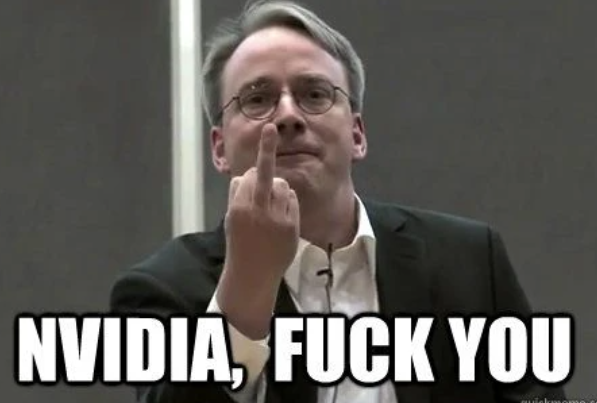
\includegraphics[width=0.9\textwidth,keepaspectratio]{assets/Linux/Hello Linux!/2.png}
\end{figure}

\subsection*{\textbf{Why Linux}}

As a matter of fact, Linux is convenient, isn't it? And
sometimes you know, there are lots of course designs that force you to
use Linux to run programs which can have run on Windows. So, as a
Windows user with 10+ years of experience, I (and also you) have to
learn to use Linux instead.

Moreover, I know some of you will take part in competitions about
robots, All of these test your Linux usage ability. For example, raspi,
nano, they mainboards is controlled through Linux. Essential, right?

\subsection*{\textbf{Which Linux}}

\begin{figure}[H]
    \centering
    
\includegraphics[width=0.9\textwidth,keepaspectratio]{assets/Linux/Hello Linux!/3.png}
\end{figure}

There are always people debating which Linux distribution is better.
Actually in my opinion most of them are similar, and the kernel commands
are all the same.

For we newbies, I suggest Debian.\ \texttt{KDE}\ desktop is beautiful and
highly customizable. The whole OS is stable enough to be used until
death. And the most important is that you can find tutorials easier than
Archlinux or Redhat when getting troubles.

\begin{mdquote}
Why not Ubuntu? Check \textbf{2.7 I'd rather be a
bookworm}!
\end{mdquote}

\subsection*{\textbf{At last}}

Rome is not built in a day, and Linux can't be learnt at
once. It's like your school courses which needs to
review and improve constantly. Maybe it's not useful at
the moment, like calculus cannot be used to buy groceries either. It
WILL make a huge impact one day. Now let's say the
famous saying. \emph{Talk is cheap, show me the code!}

\newpage
\thispagestyle{empty}
\begin{center}
    \vspace*{96pt}
    \fontsize{60}{60}\customfont{1}\par
    \fontsize{26}{31.2}\section{\textbf{Basic Commands}}\par % 标题
    \vspace{25pt}
    \fontsize{18}{21.6}\customfont{\textit{Value your freedom or you will lose it, teaches history. ---RMS}}\par % 名言
    \vfill
\end{center}

\fontsize{12}{14}
\newpage
\subsection{\textbf{How to install Debian on Windows}}

\subsubsection{\textbf{VMware didn't meet my expectation}}
Yes, I used VMware to load my Ubuntu (and also my Windows Server 2019
before). Not many reasons for me but easy and fast. There are still 2
Ubuntus in my VMware, one is used to finish the computer program course
design, the other is for ISCC 2024.

However, I must say that VMware is troublesome, bugs, errors, I could
see those almost every week when I had to use it. The only exciting
thing to me may be a free cd-key when I was still in high school and
penniless. But this year they said VMware would be totally free for
individuals, so no reason to use this awful software anymore I think.

If you must use VMware, see the link below, it contains Debian 12:
\href{https://mirrors.ustc.edu.cn/debian-cd/current/amd64/iso-cd/debian-12.9.0-amd64-netinst.iso}{https://mirrors.ustc.edu.cn/debian-cd/current/amd64/iso-cd/debian-12.9.0-amd64-netinst.iso}

\begin{figure}[H]
    \centering
    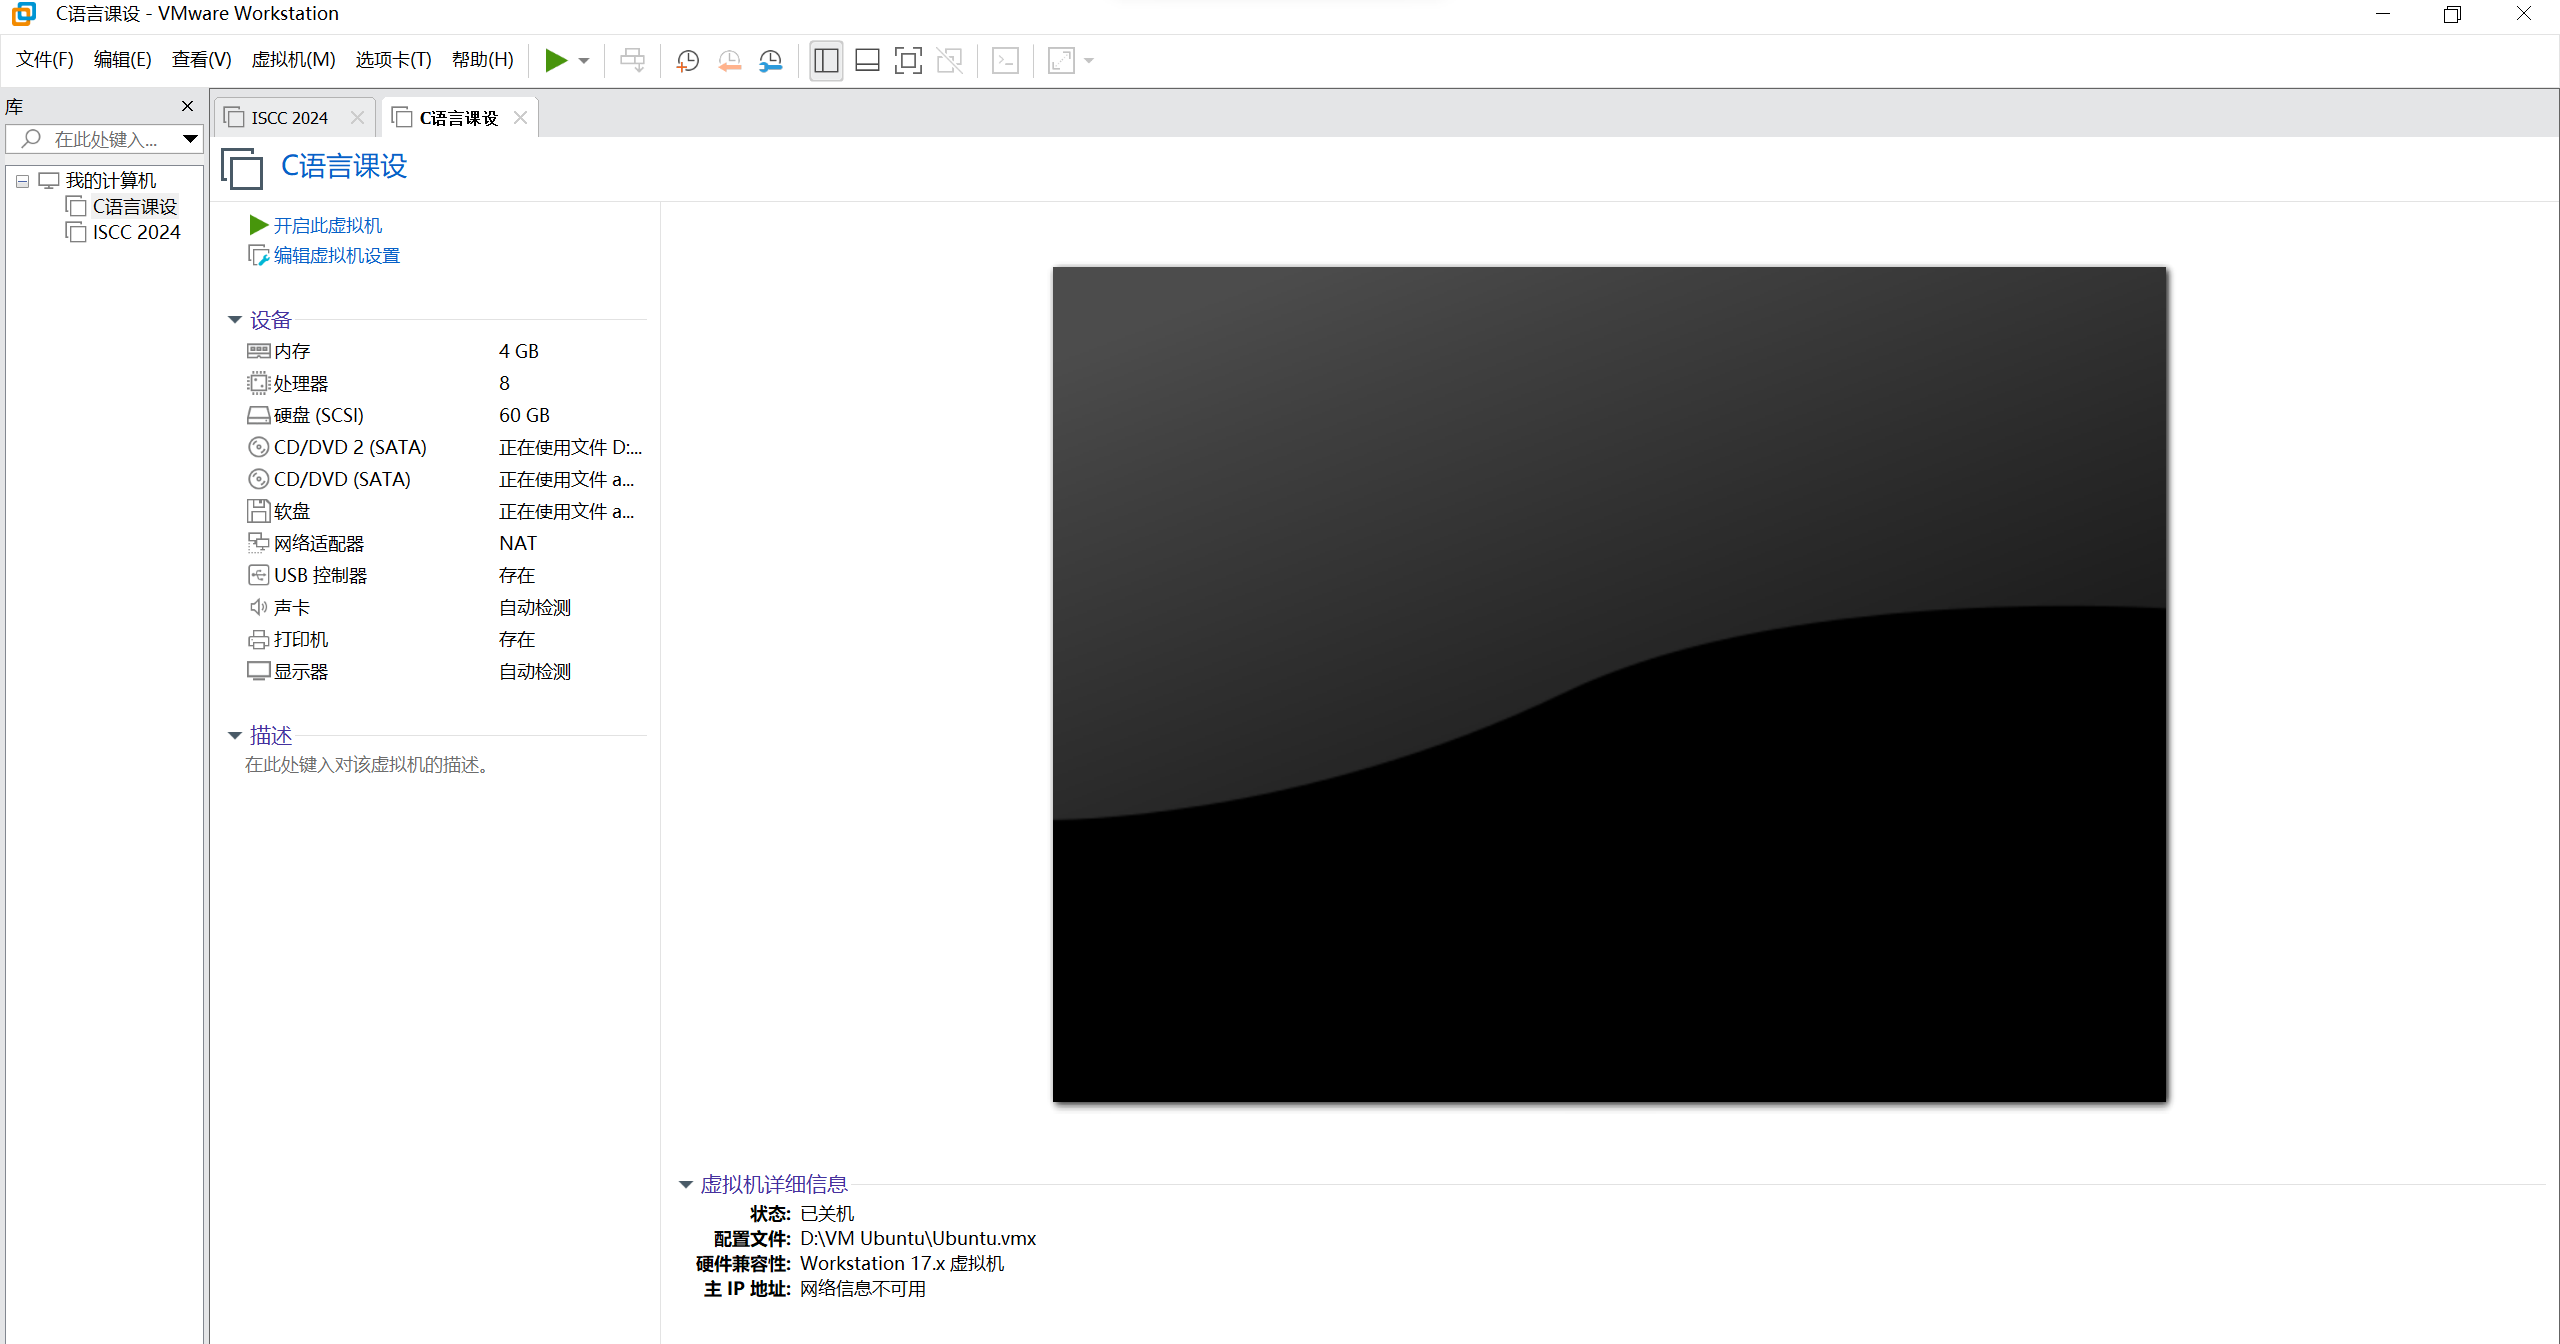
\includegraphics[width=0.9\textwidth,keepaspectratio]{assets/Linux/1.1 How to install Debian on Windows/1.png}
\end{figure}

\subsubsection{\textbf{WSL}}

No doubt that GUI is familiar to us Windows users, but not exactly to
Linuxer. Try using an OS with only terminal is hard but interesting.
Then WSL is the best choice.

I will give an example that installing Debian 12 on Windows 11.

\subsubsection*{\textbf{An example}}

Press \texttt{Win\ +\ R}\ and input \texttt{optionalfeatures}, click 
\texttt{Windows\ subsystem\ for\ Linux}\ and \texttt{Virtual\ Machine\ Platform}.

\begin{figure}[H]
    \centering
    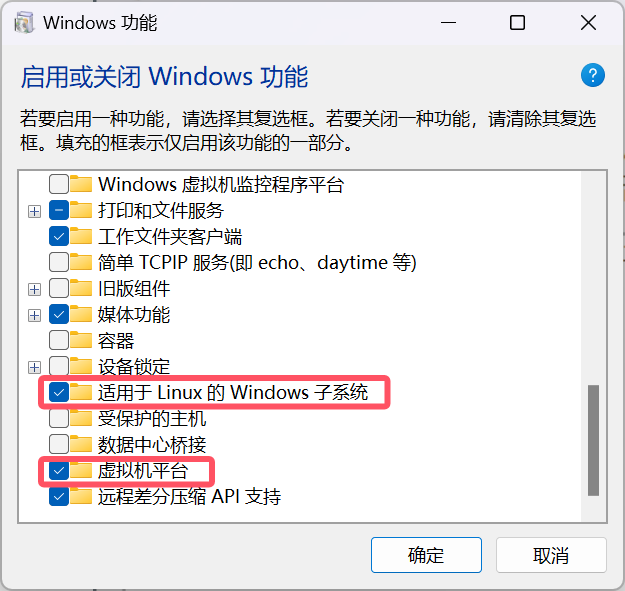
\includegraphics[width=0.9\textwidth,keepaspectratio]{assets/Linux/1.1 How to install Debian on Windows/2.png}
\end{figure}

Open Microsoft Store, download Debian 12.

\begin{figure}[H]
    \centering
    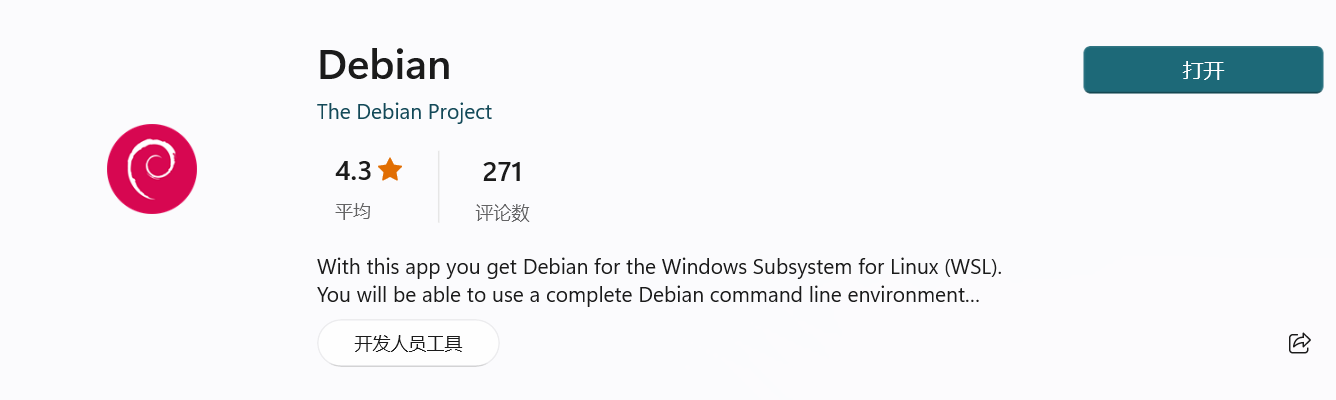
\includegraphics[width=0.9\textwidth,keepaspectratio]{assets/Linux/1.1 How to install Debian on Windows/3.png}
\end{figure}
Press \texttt{Win\ +\ R}\ and input \texttt{wt}, input
\texttt{wsl -update}, then you can use Linux on Windows.

\begin{figure}[H]
    \centering
    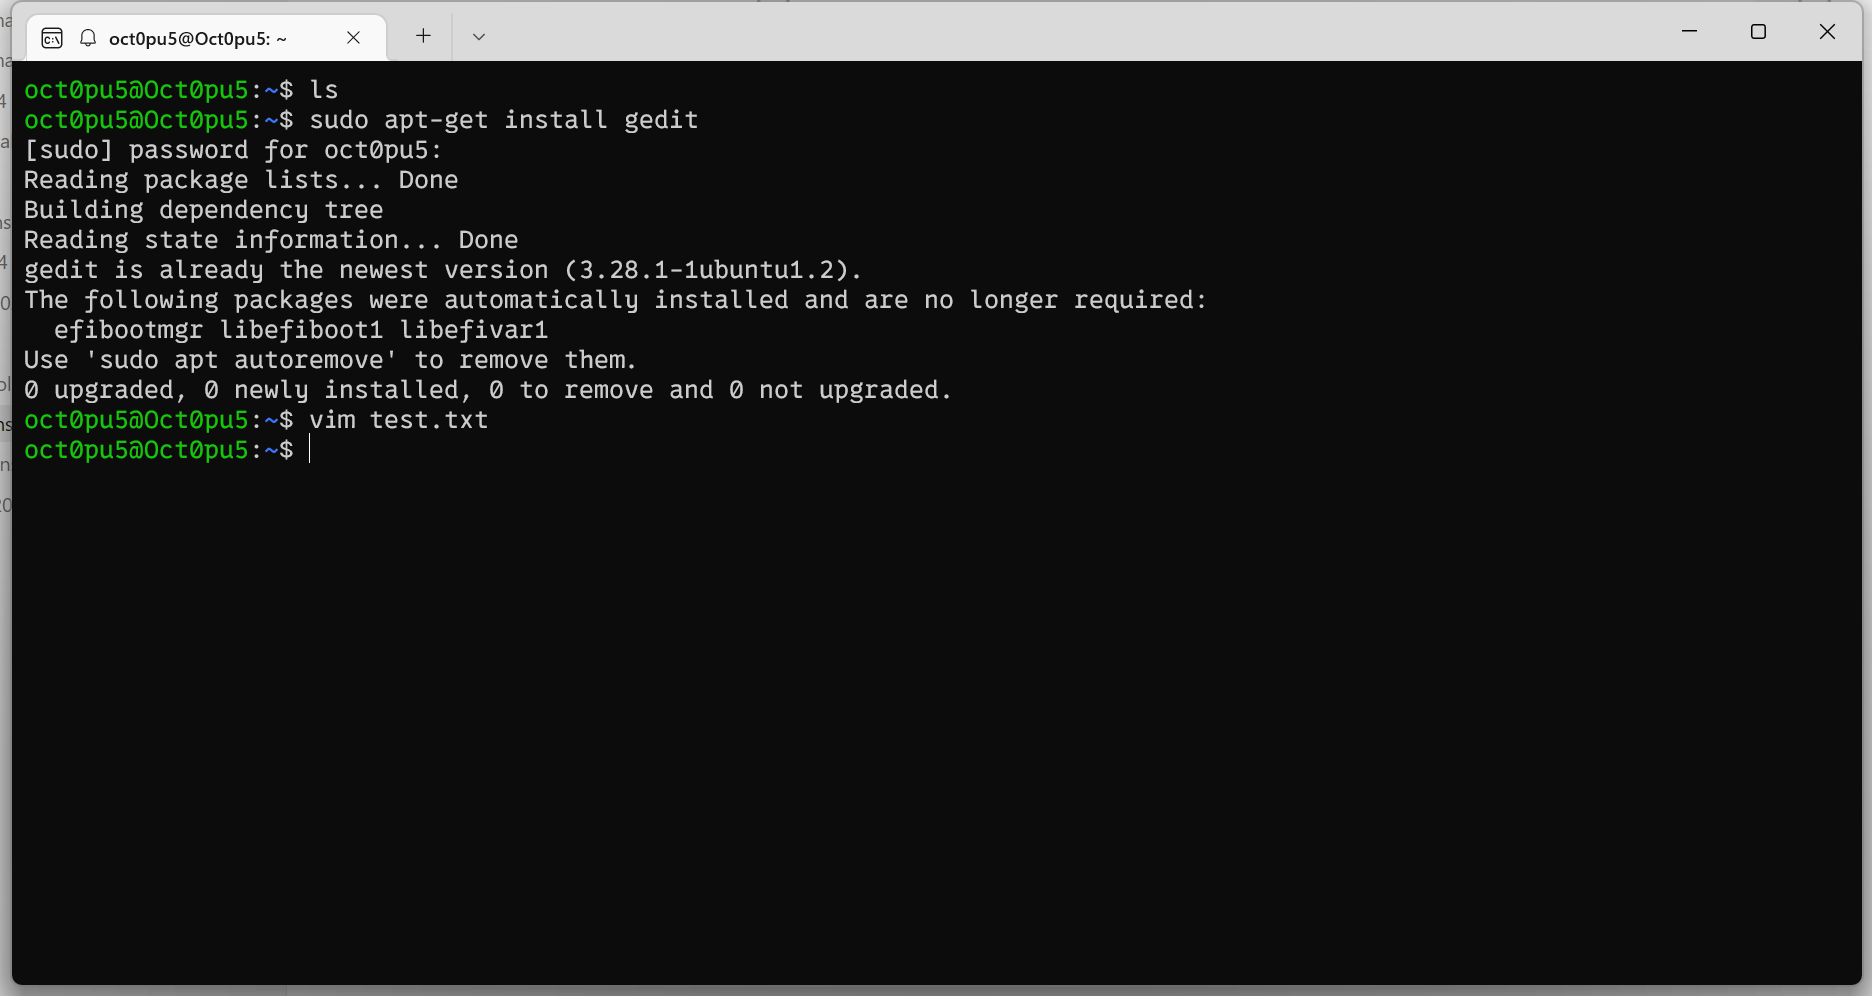
\includegraphics[width=0.9\textwidth,keepaspectratio]{assets/Linux/1.1 How to install Debian on Windows/4.png}
\end{figure}

Then connect your Debian with VSCode. Download \texttt{WSL}\ extension,
connect to your Debian.

\begin{figure}[H]
    \centering
    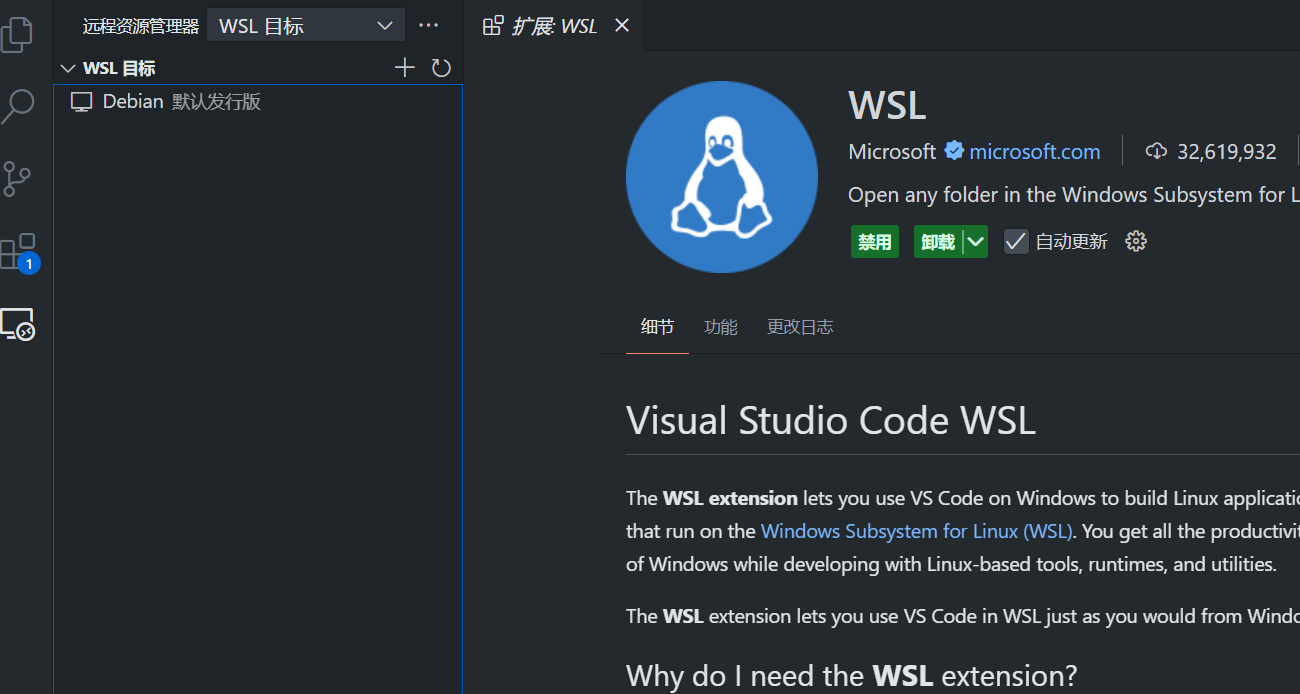
\includegraphics[width=0.9\textwidth,keepaspectratio]{assets/Linux/1.1 How to install Debian on Windows/5.png}
\end{figure}

Now you can use VSCode to edit files what ever you want.

\subsubsection*{\textbf{Notice}}

If you want to call VSCode in the terminal, just input \texttt{code\ ..}

\begin{figure}[H]
    \centering
    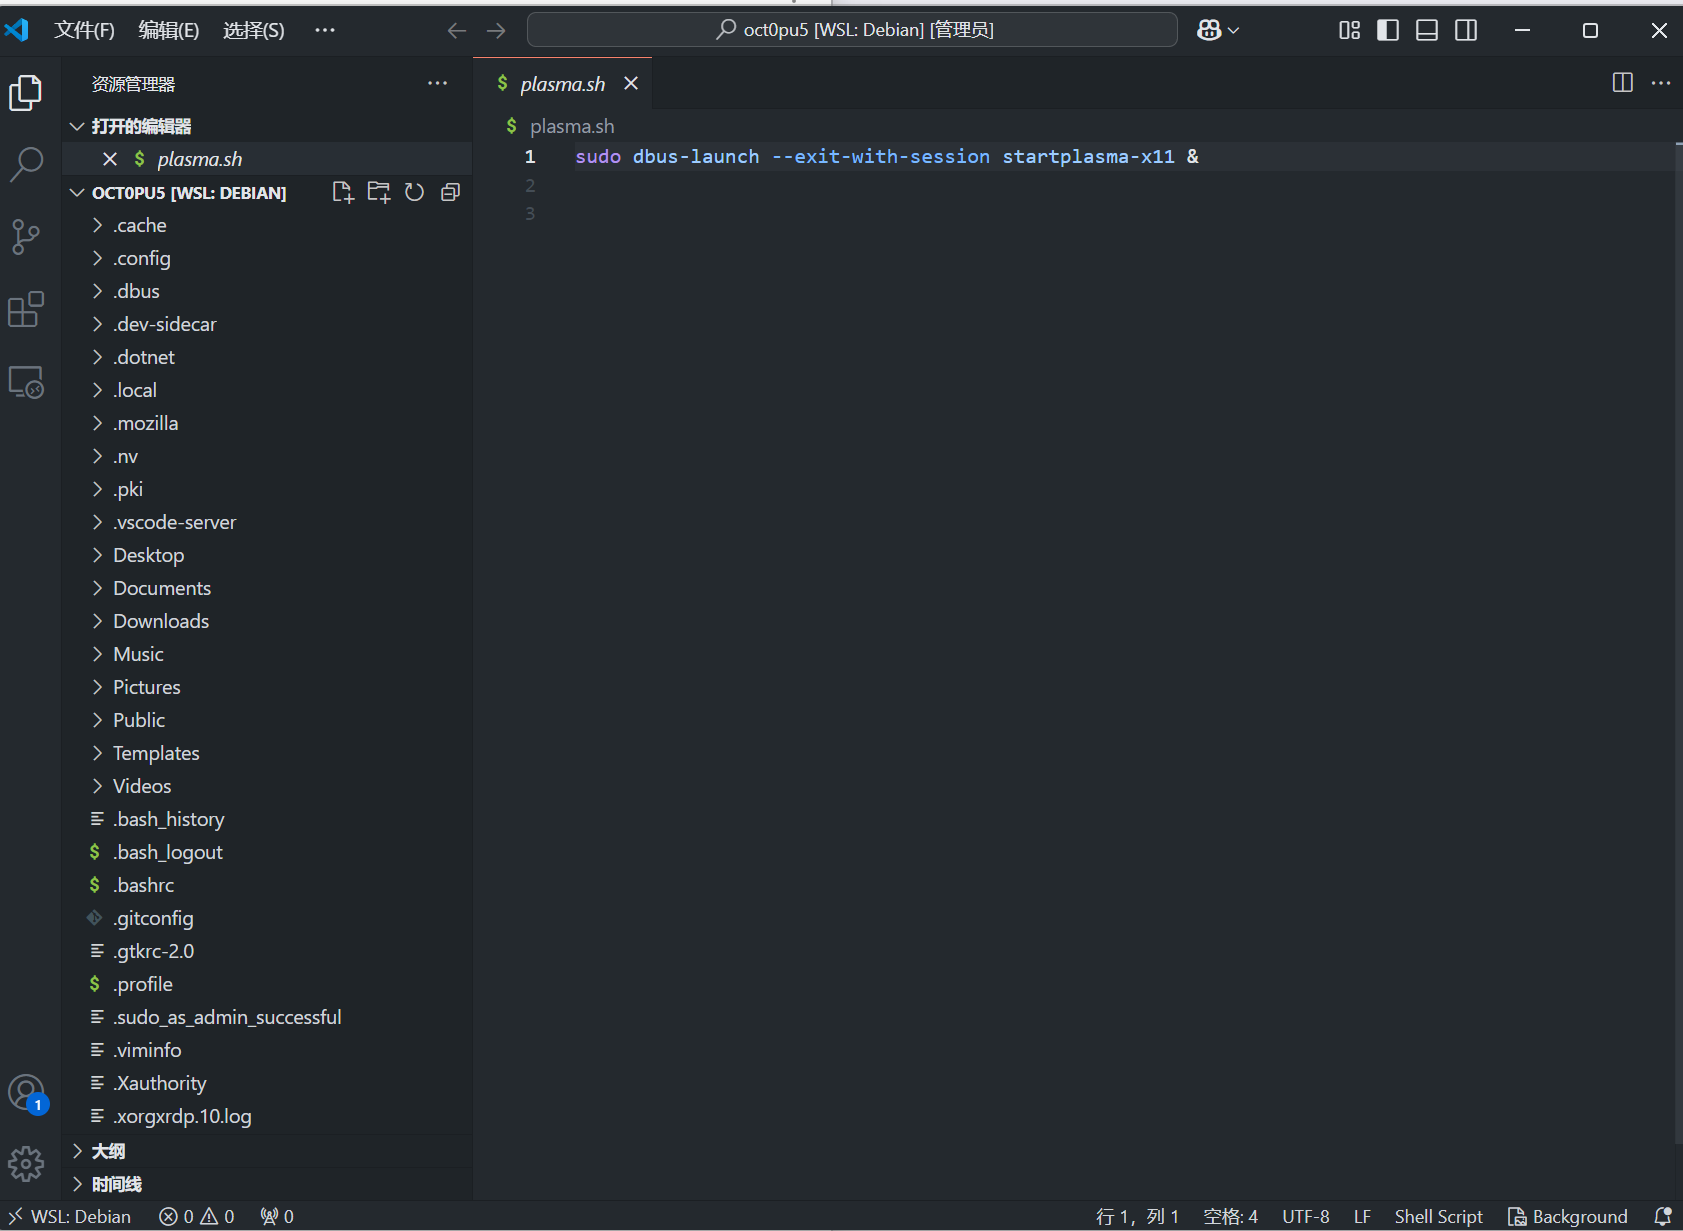
\includegraphics[width=0.85\textwidth,keepaspectratio]{assets/Linux/1.1 How to install Debian on Windows/6.png}
\end{figure}

You can also check files here:

\begin{figure}[H]
    \centering
    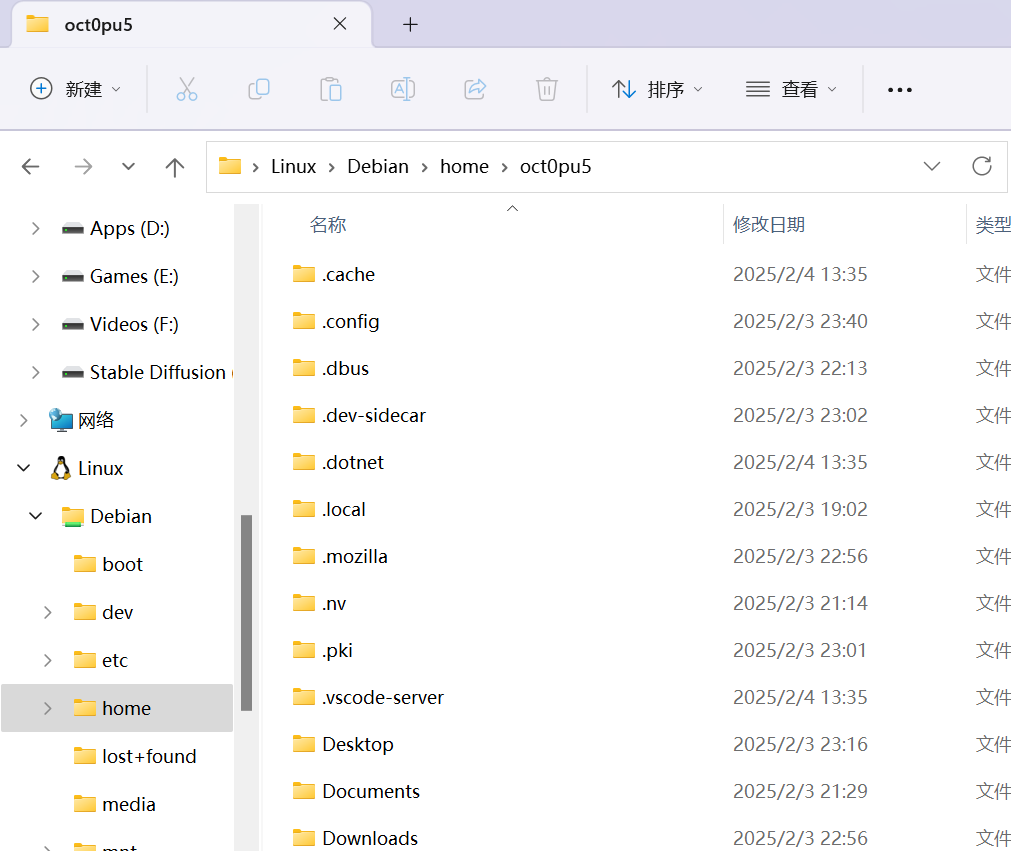
\includegraphics[width=0.85\textwidth,keepaspectratio]{assets/Linux/1.1 How to install Debian on Windows/7.png}
\end{figure}

\subsection{\textbf{C++ \& Python Environment Configuration on Linux}}

\subsubsection{\textbf{C++}}

\begin{adjustwidth}{2em}{0pt}
\begin{verbatim}
sudo apt update
sudo apt install build-essential
\end{verbatim}
\end{adjustwidth}

\texttt{build-essential}\ contains packages which C++ programs need such
as \texttt{gcc},\ \texttt{g++},\ \texttt{cmake}, etc.

If you have edited a file \texttt{hello.cpp}, then you can compile and
run it.

\begin{adjustwidth}{2em}{0pt}
\begin{verbatim}
g++ hello.cpp -o hello
./hello
\end{verbatim}
\end{adjustwidth}

\begin{mdquote}
If you have problems when downloading dependencies of \texttt{g++}, check
\textbf{10 Linux network commands}\ first then contact me.
\end{mdquote}

\subsubsection{\textbf{Python}}

\begin{mdquote}
Don't use Python2, it has outdated!
\end{mdquote}

\begin{adjustwidth}{2em}{0pt}
\begin{verbatim}
sudo apt update
sudo apt install python3
sudo apt install python3-pip
\end{verbatim}
\end{adjustwidth}

Remember, there are differences between Windows and Linux. You need to
input \texttt{python3},\ \texttt{pip3}\ instead of \texttt{python},\
\texttt{pip}.

\subsection{\textbf{How to edit files on Linux}}

\subsubsection{\textbf{Brief}}

We install Linux, aiming to write codes. Then we must know how to edit
files.

On Windows, we can use lots of tools such as \texttt{notepad},
\texttt{Devcpp},\ \texttt{VSCode},\ \texttt{Pycharm}, etc. However,
it's not the same as Linux. Linux don't
have a \texttt{notepad} anyway. At our current level, I advise you only
1 way named \texttt{Vim}.

\begin{mdquote}
As for my personal experience, \texttt{Vim}\ is the best editor on Linux.
And you can see more skills about \texttt{Vim}\ in 
\textbf{2.9 Having heard Dao in the morning}.
Why I don't mention \texttt{Emacs} in this tutorial? Because I never use it xD
\end{mdquote}

\begin{figure}[H]
    \centering
    
\includegraphics[width=0.9\textwidth,keepaspectratio]{assets/Linux/1.3 How to edit files on Linux/1.png}
\end{figure}

\subsubsection{\textbf{Vim}}

Run commands below to install:

\begin{adjustwidth}{2em}{0pt}
\begin{verbatim}
sudo apt update
sudo apt install vim
\end{verbatim}
\end{adjustwidth}

When editing files, just input \texttt{vim\ yourfilename}. If
doesn't exist, \texttt{Vim}\ will open a new file for
you. Here is the interface.

\begin{figure}[H]
    \centering
    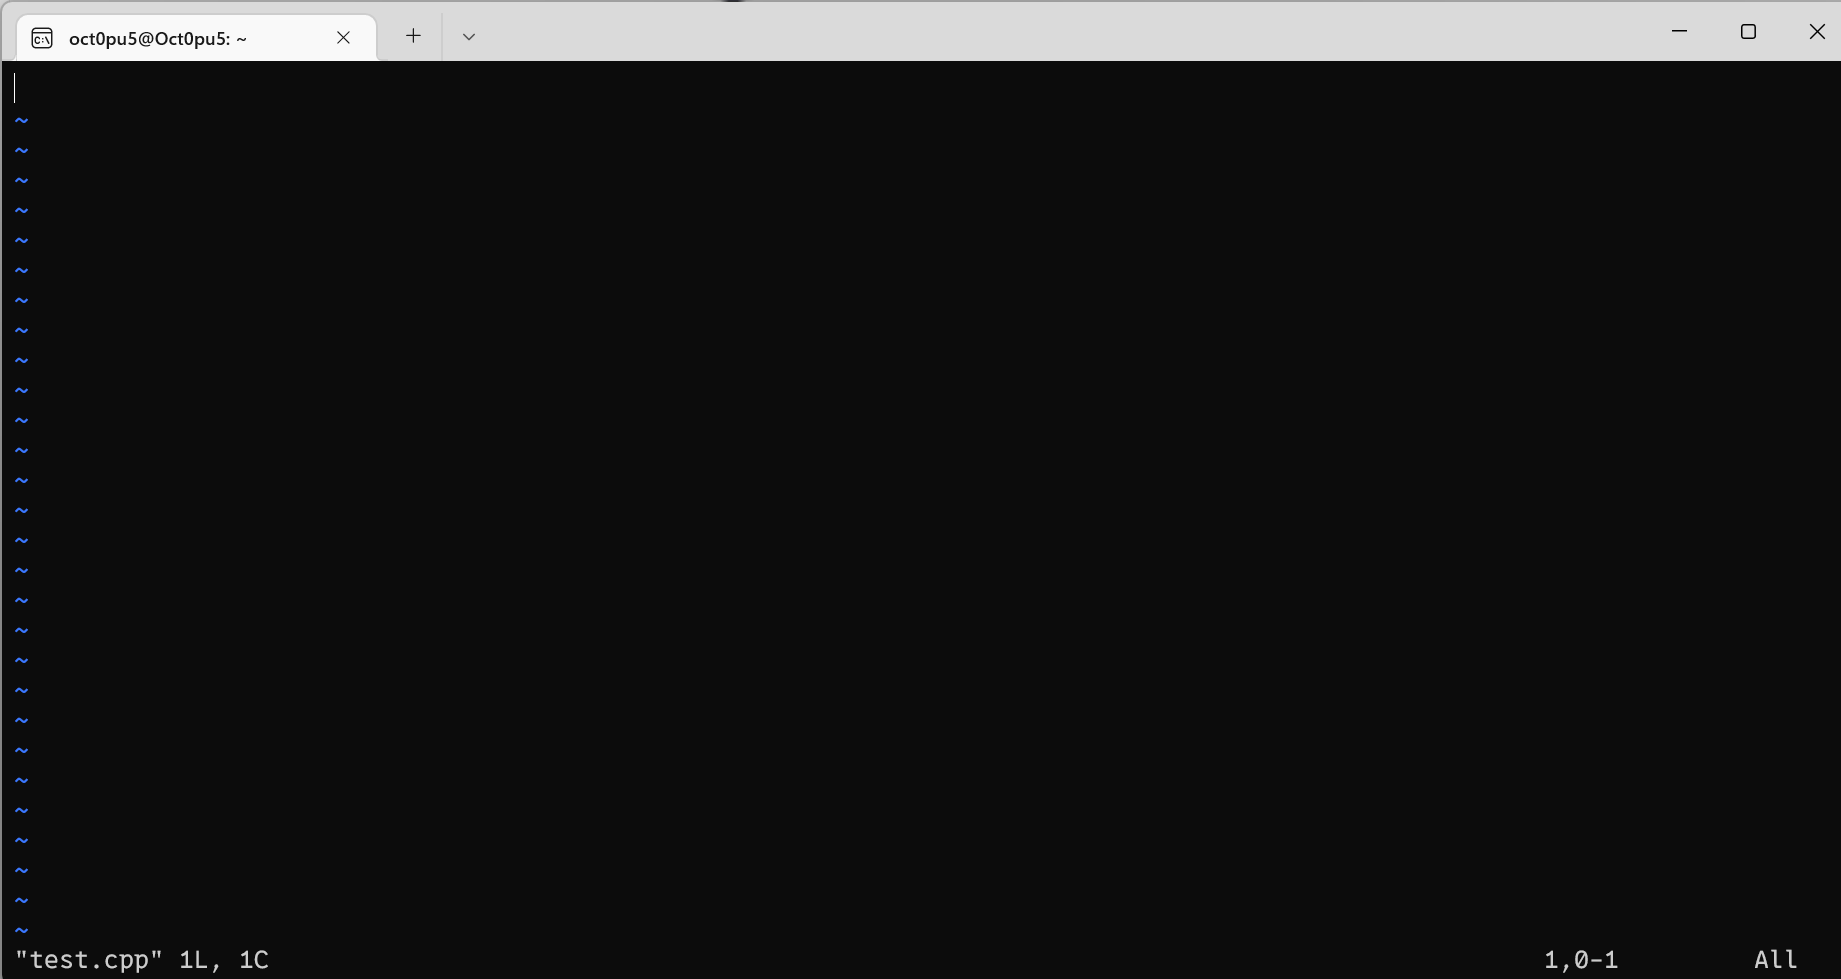
\includegraphics[width=0.9\textwidth,keepaspectratio]{assets/Linux/1.3 How to edit files on Linux/2.png}
\end{figure}

\texttt{Vim}\ has 2 input modes and many different methods. Here, we only
need to know the most commonly used insertion mode. Press \texttt{i}\ and
you should see \texttt{-\/-INSERT-\/-}\ in the bottom left corner. After
this, input and delete whatever you want!

When you think all is done, press \texttt{esc}\ to quit insertion mode,
then input \texttt{:wq}\ to save and quit \texttt{Vim}.

\begin{figure}[H]
    \centering
    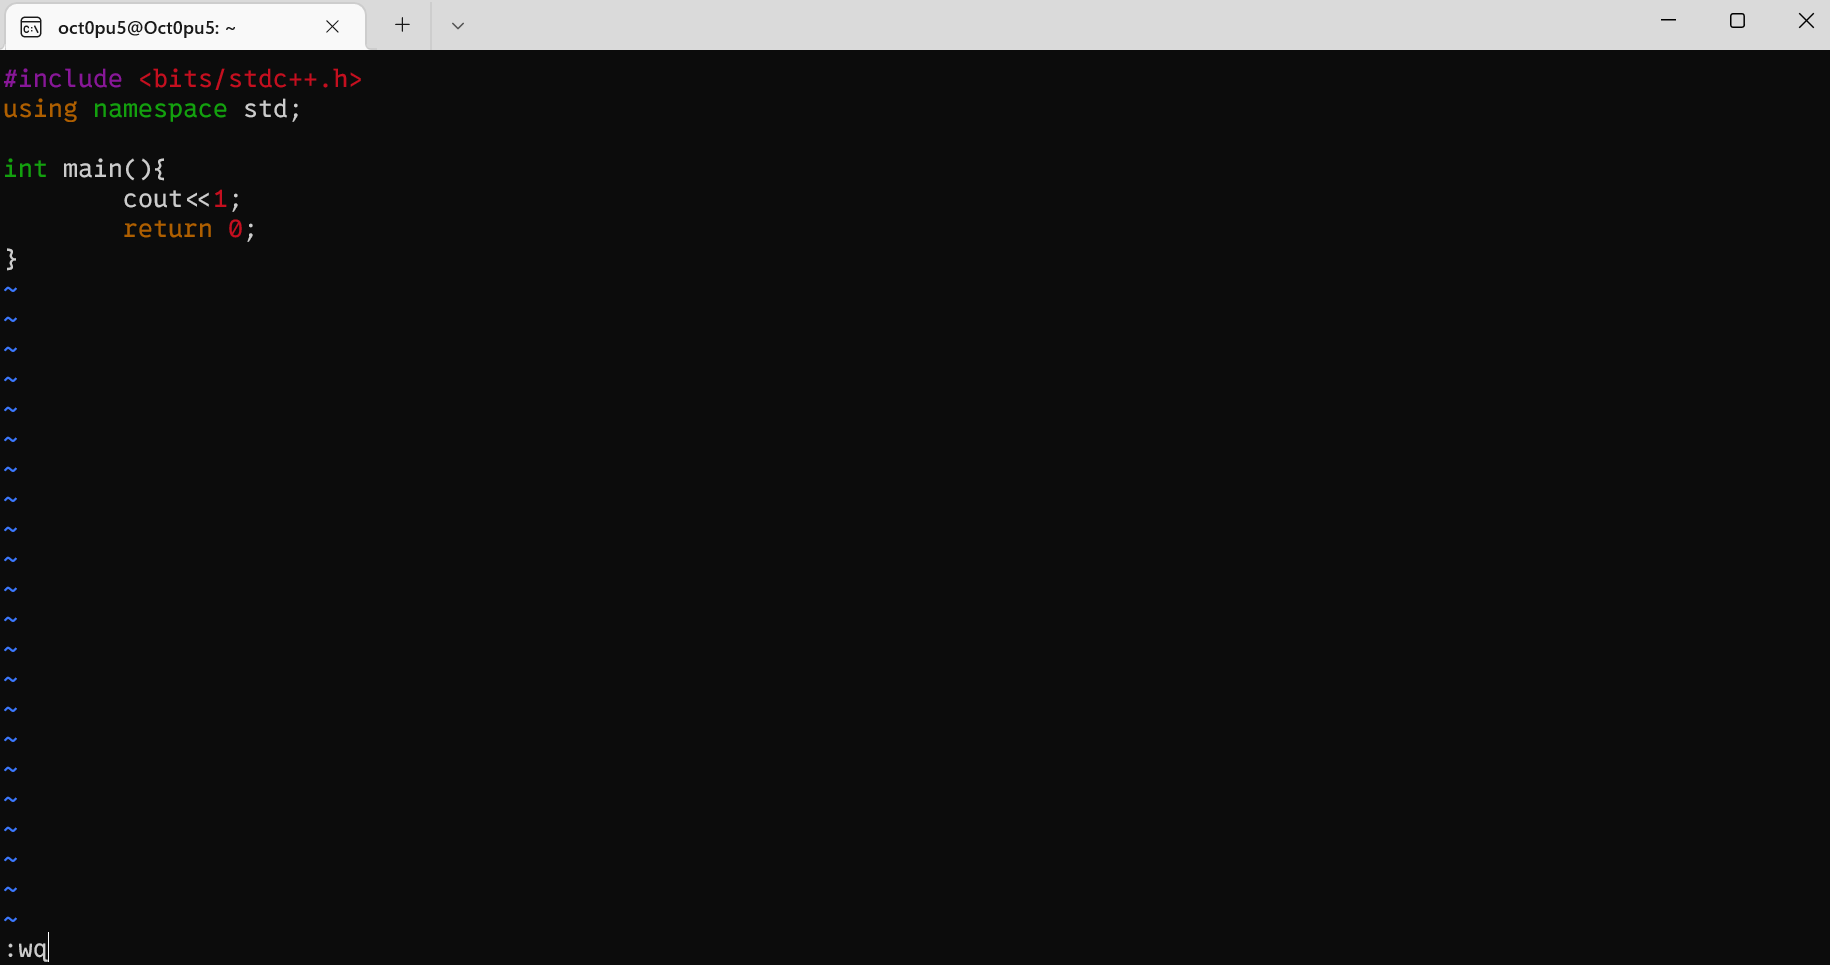
\includegraphics[width=0.9\textwidth,keepaspectratio]{assets/Linux/1.3 How to edit files on Linux/3.png}
\end{figure}

This is a table that lists various inputs and their functions.

\begin{table}[H]
    \centering
    \begin{tabular}{cc}
    \toprule
    Input & Functions \\
    \midrule
    :wq & save and quit \\
    :q & cancel and quit \\
    :q! & cancel and force quit \\
    :e! & cancel and open the original file \\
    \bottomrule
    \end{tabular}
\end{table}

Sometimes you need to find a function or variable in massive codes. On
Windows \texttt{Ctrl+F}\ helps you. Also, \texttt{Vim}\ has this ability.
Just input \texttt{/whatyousearch}. Take a look at this example below:

\begin{figure}[H]
    \centering
    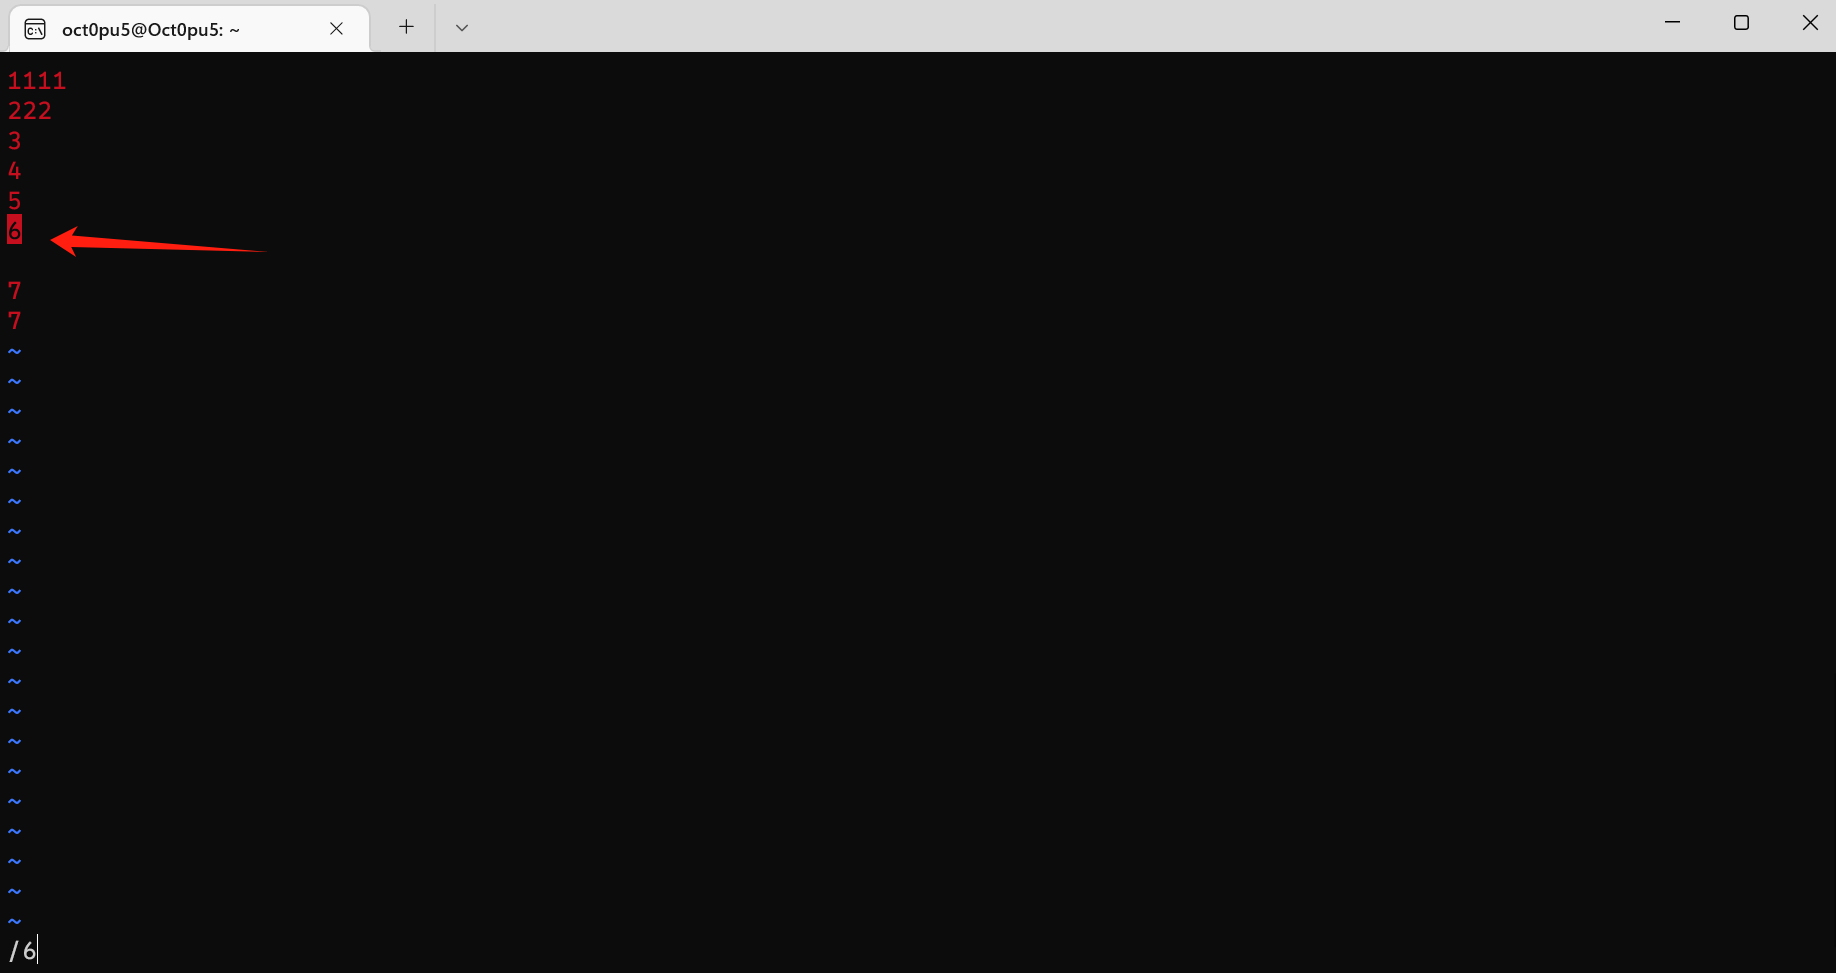
\includegraphics[width=0.9\textwidth,keepaspectratio]{assets/Linux/1.3 How to edit files on Linux/4.png}
\end{figure}

\subsubsection{\textbf{Other Tools}}

\subsubsection*{\textbf{nano}}

\begin{figure}[H]
    \centering
    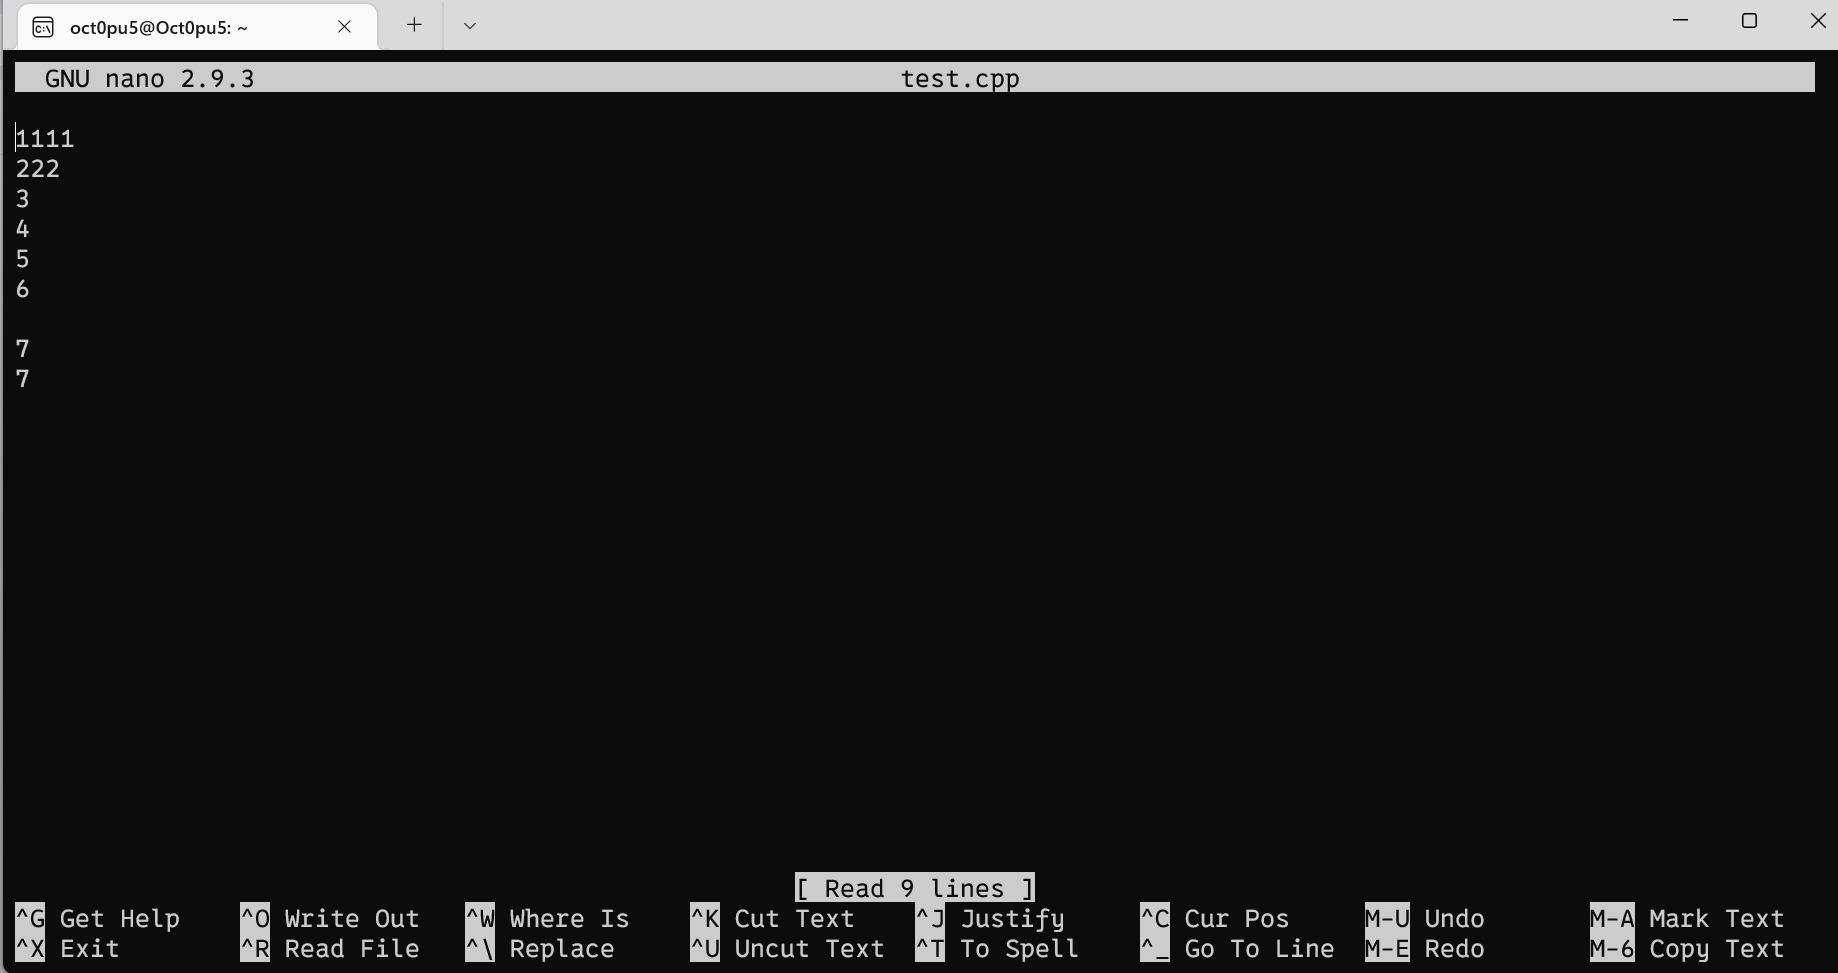
\includegraphics[width=0.9\textwidth,keepaspectratio]{assets/Linux/1.3 How to edit files on Linux/5.png}
\end{figure}

\texttt{nano} is another editor besides \texttt{Vim}, I
don't like it because \texttt{Vim}\ is more powerful than
it nearly in all aspects. If you want to learn \texttt{nano}, check this
tutorial:
\url{https://blog.csdn.net/f272935657/article/details/141575478}.

\subsubsection*{\textbf{Gedit}}

\texttt{Gedit}\ is a light text editor. It supports various languages and
its graphical interface is more like \texttt{notepad}, making it more
user-friendly for \texttt{Windows} users.

However, \texttt{Gedit}\ has bugs for Linux without GUI, these warnings
often make users puzzled (although it IS simple and will cause no
mistake). So I won't use it anyway.

\begin{figure}[H]
    \centering
    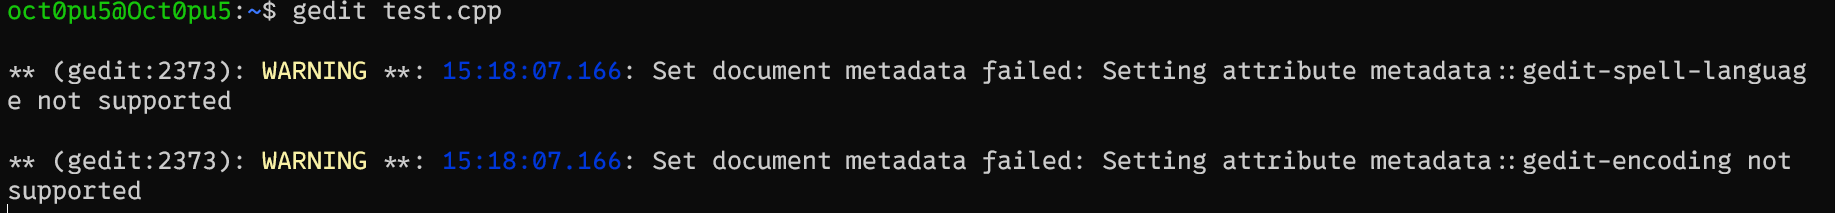
\includegraphics[width=0.9\textwidth,keepaspectratio]{assets/Linux/1.3 How to edit files on Linux/6.png}
\end{figure}

If you want to install \texttt{Gedit}, follow the commands below:

\begin{adjustwidth}{2em}{0pt}
\begin{verbatim}
sudo apt upgrade
sudo apt install gedit
gedit yourfilename
\end{verbatim}
\end{adjustwidth}

It should be like this:

\begin{figure}[H]
    \centering
    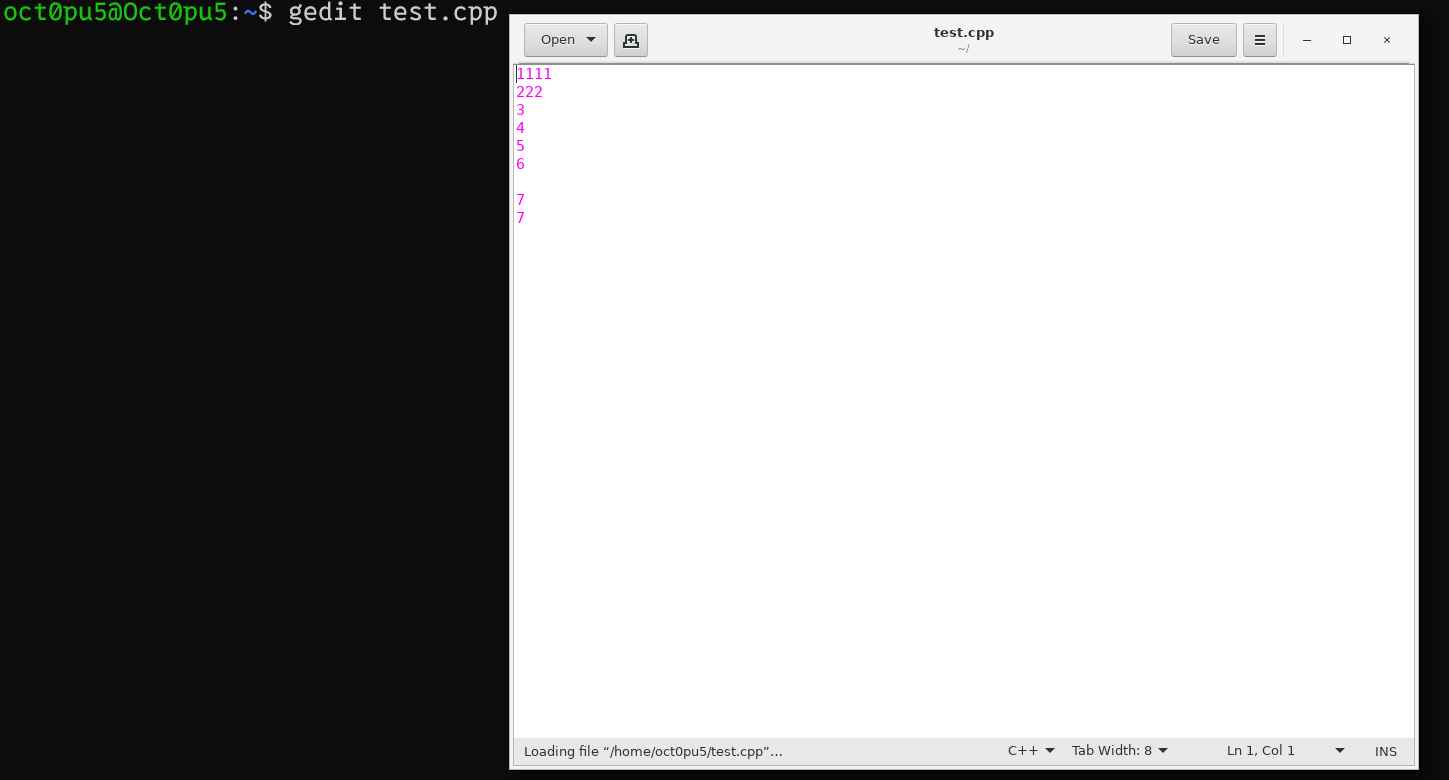
\includegraphics[width=0.9\textwidth,keepaspectratio]{assets/Linux/1.3 How to edit files on Linux/7.png}
\end{figure}

\newpage
\subsection{\textbf{Directory structure}}

\subsubsection{\textbf{Top level directory}}

As we all know, There are some drives on Windows, we call them
\texttt{top\ level\ directory}, such as \texttt{C:\textbackslash{}},
\texttt{D:\textbackslash{}}, etc. However, Things are quite different on
Linux. There is only 1 \texttt{top\ level\ directory}\ named \texttt{/}.
And we often call this directory structure \texttt{tree}.

You must notice that the symbols representing hierarchical relationships
are different on Windows and Linux. Actually \texttt{\textbackslash{}}\
on Windows and \texttt{/}\ on Linux. It's very easy to
confuse so recite it by heart.

\subsubsection{\textbf{Absolute path and relative
path}}

I have taught this part in HTML tutorial, but still need to emphasize
again.

Absolute path starts with \texttt{/}, and relative path starts with
current directory. In actual operation we use relative path more often.

Assume we have following directory structure:

\begin{adjustwidth}{2em}{0pt}
\begin{verbatim}
home/
|—— test.cpp
|—— README.md
|—— LICENSE
\end{verbatim}
\end{adjustwidth}

Here are 2 examples showing what're absolute path and
relative path:

To represent \texttt{test.cpp}in absolute path, It's
\texttt{/home/test.cpp}. And for \texttt{LICENSE}, we use relative path
\texttt{LICENSE} (This is relative to \texttt{test.cpp})

Isn't it very simple? For beginners,
it's easy to make mistakes. Make sure to memorize it.

\subsubsection{\textbf{Special path symbols}}

Linux provides 3 \texttt{Special\ path\ symbols} for users to write file
path easier. I list them in a form.

\begin{table}[H]
    \centering
    \begin{tabular}{cc}
    \toprule
    symbol & meaning \\
    \midrule
    \texttt{.} & Current directory \\
    \texttt{..} & Previous level directory \\
    \texttt{\textasciitilde{}} & \texttt{/home} \\
    \bottomrule
    \end{tabular}
\end{table}
I will explain them in more detail in the following text.

\subsubsection{\textbf{Directory Commands}}

\subsubsection*{\textbf{ls}}

\texttt{ls}\ list files in current directory. Here's its
grammar: \texttt{ls\ {[}-a\ -h\ -l{]}\ {[}path{]}}.

If you choose no parameter, \texttt{ls}\ represents displaying files in a
flat layout.

\begin{figure}[H]
    \centering
    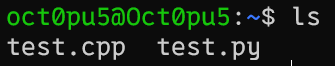
\includegraphics[width=0.9\textwidth,keepaspectratio]{assets/Linux/1.4 Linux directory structure and command/1.png}
\end{figure}

\texttt{-a} means show all files include those are hidden.
It's easy to hide files on Linux, just add a \texttt{.}\
before its name such as \texttt{.bashrc}.

\begin{figure}[H]
    \centering
    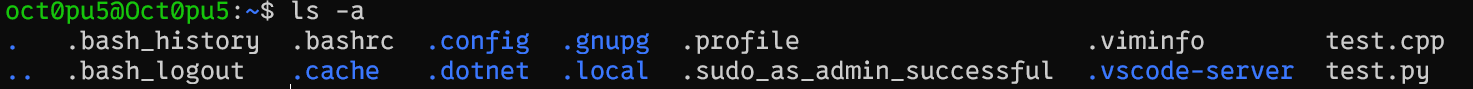
\includegraphics[width=0.9\textwidth,keepaspectratio]{assets/Linux/1.4 Linux directory structure and command/2.png}
\end{figure}

\begin{mdquote}
Files and folders are distinguished by color in WSL, those blue names
are folders.
\end{mdquote}

\texttt{-l}\ means show files in a column with more information like
'detailed information' on Windows.

\texttt{-h}\ changes \texttt{file\ size}\ in \texttt{-l}\ to clearer style
(represent by \texttt{k},\ \texttt{m},\ \texttt{g}) and \textbf{must use
with -l}

\begin{figure}[H]
    \centering
    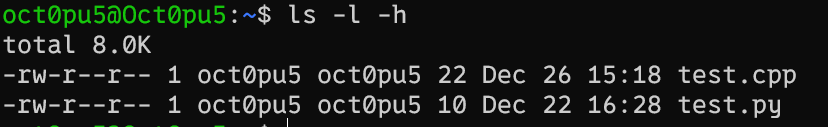
\includegraphics[width=0.9\textwidth,keepaspectratio]{assets/Linux/1.4 Linux directory structure and command/3.png}
\end{figure}

\begin{mdquote}
Parameters above can be put together like \texttt{-alh}.
\end{mdquote}

As for \texttt{path}\ parameter, we often take following strategy: switch
to the desired directory and \texttt{ls}\ rather than
\texttt{ls\ desireddirectory}\ directly, so I won't teach
it xD

\subsubsection*{\textbf{cd}}

As the same as \texttt{cd}\ on Windows Terminal, its function is
\textbf{c}hange \textbf{d}irectory. Grammar here:
\texttt{cd\ {[}path{]}}.

There's not much to say, just pay attention to one thing
that \texttt{cd}\ default path is \texttt{/home}. That means \texttt{cd}\
equals \texttt{cd\ \textasciitilde{}} and if there's a
\texttt{/home/test.cpp}, you just need to \texttt{cd\ test.cpp}.

Now we finished \texttt{cd}, it's time to talk about
details that weren't clear in the previous text.

As for me, \texttt{..}\ is often used in \texttt{cd}. See the figure
below, \texttt{cd}\ default path is \texttt{/home/oct0pu5}. I input
\texttt{cd\ ..}\ twice and return \texttt{/}, then \texttt{cd\ etc}\ and
\texttt{ls}, it shows all file in \texttt{/etc}. The above is the
classic directory operation.

\begin{figure}[H]
    \centering
    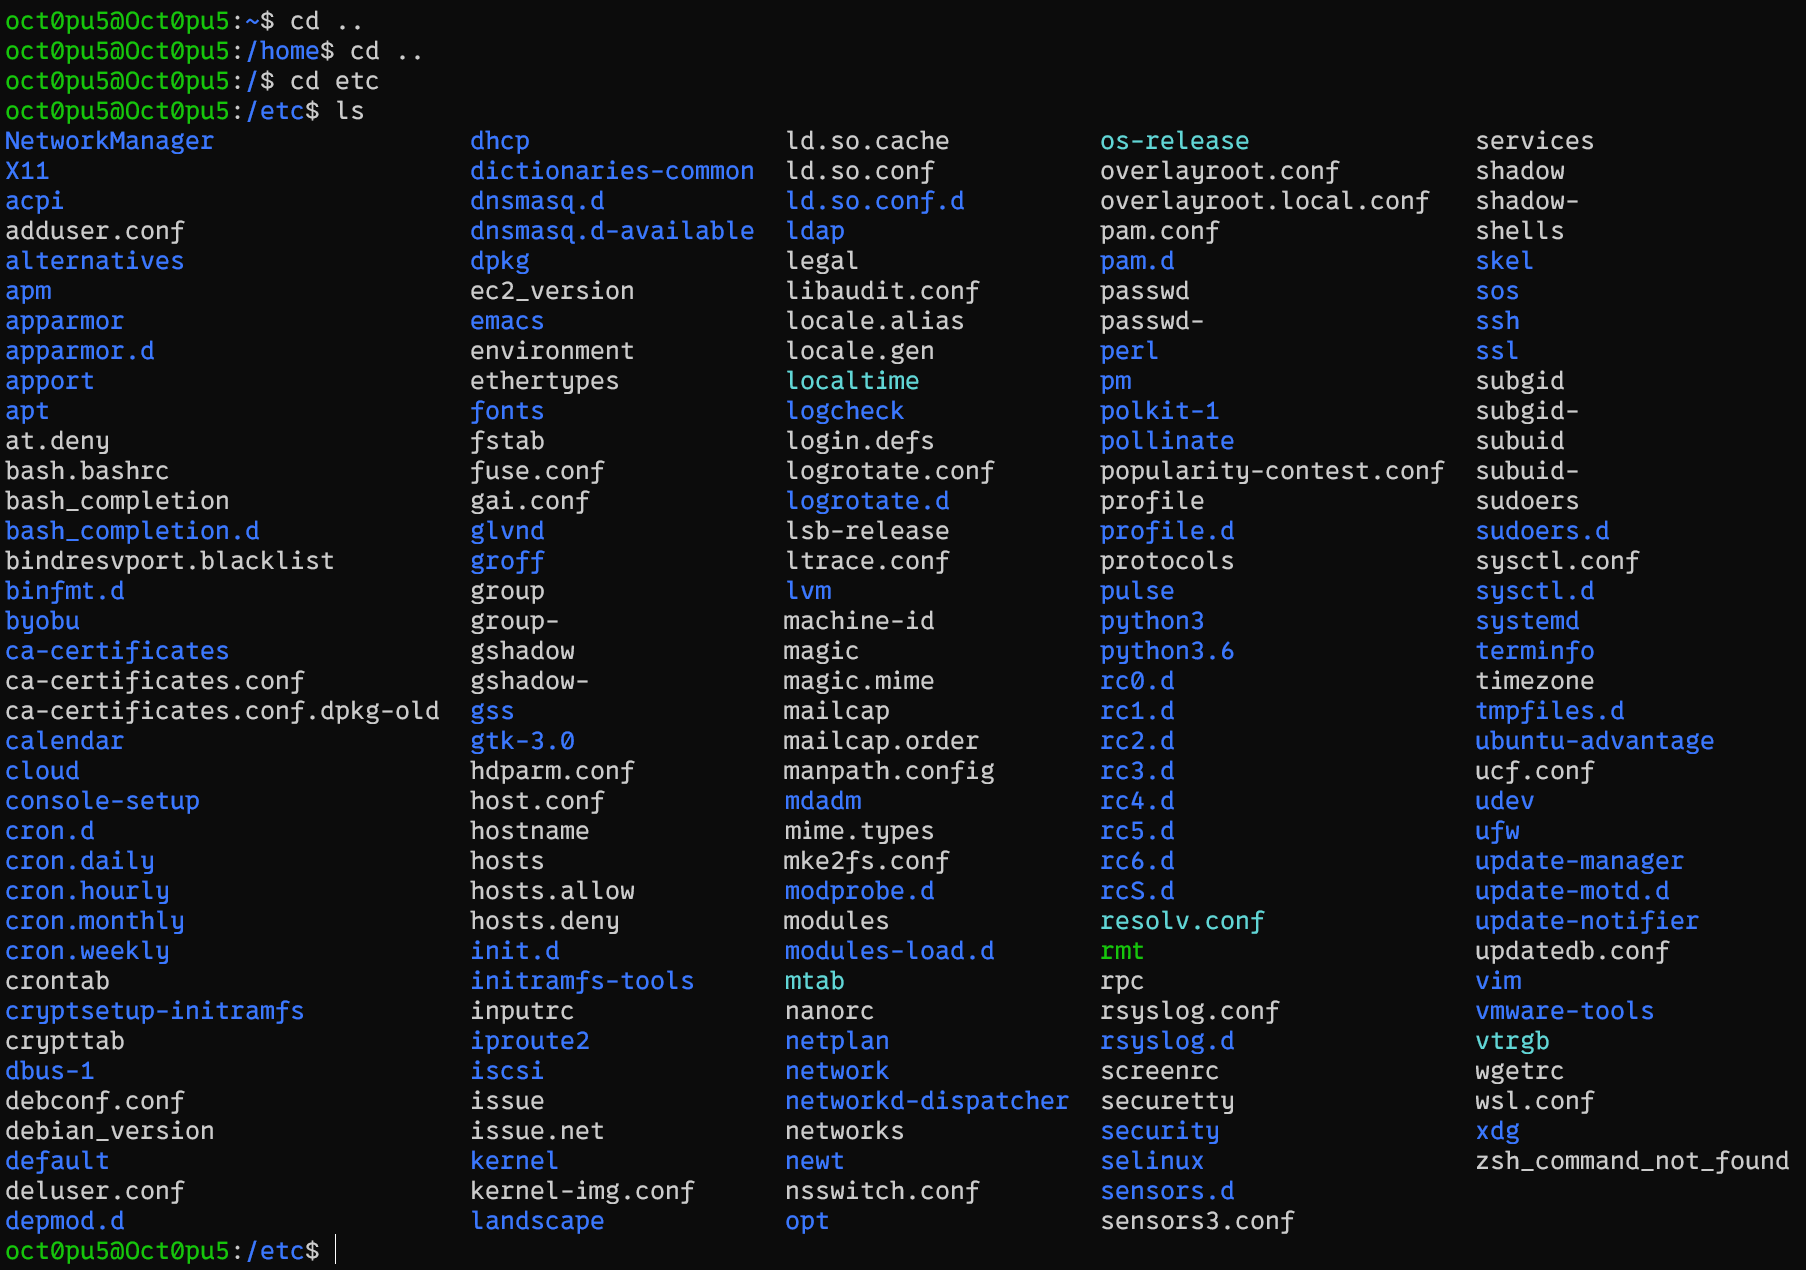
\includegraphics[width=0.9\textwidth,keepaspectratio]{assets/Linux/1.4 Linux directory structure and command/4.png}
\end{figure}

\subsubsection*{\textbf{pwd}}

\textbf{P}rint current \textbf{w}ork \textbf{d}irectory. Often used to
check whether you are in right directory, or copy the directory for any
purpose.

\begin{figure}[H]
    \centering
    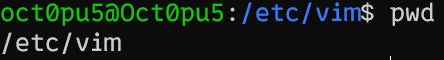
\includegraphics[width=0.9\textwidth,keepaspectratio]{assets/Linux/1.4 Linux directory structure and command/5.png}
\end{figure}

\subsubsection*{\textbf{mkdir}}

\textbf{M}a\textbf{k}e \textbf{dir}ectory. Grammar here:
\texttt{mkdir\ {[}-p{]}\ \textless{}path\textgreater{}}.

If you just want to create one level folder, ignore \texttt{-p}. If more
than one level is needed, \texttt{mkdir}\ must attach \texttt{-p},
otherwise it will throw error.

\begin{figure}[H]
    \centering
    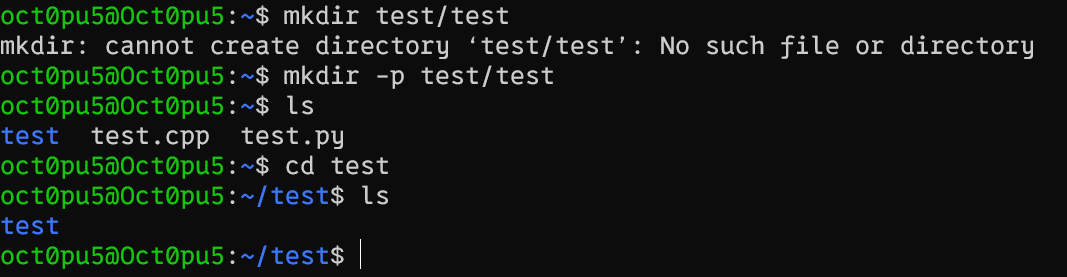
\includegraphics[width=0.9\textwidth,keepaspectratio]{assets/Linux/1.4 Linux directory structure and command/6.png}
\end{figure}

\begin{mdquote}
\texttt{mkdir} can only take effect in \texttt{/home}\ by default. We can
solve this problem in \textbf{1.6 Linux user and permission commands}.
\end{mdquote}

\begin{figure}[H]
    \centering
    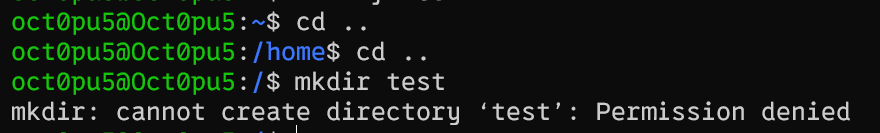
\includegraphics[width=0.9\textwidth,keepaspectratio]{assets/Linux/1.4 Linux directory structure and command/7.png}
\end{figure}

\newpage
\subsection{\textbf{Linux file commands}}
\subsubsection{\textbf{touch cat more}}

\texttt{touch} creates new file.

\begin{figure}[H]
    \centering
    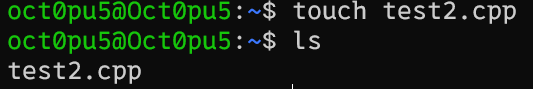
\includegraphics[width=0.9\textwidth,keepaspectratio]{assets/Linux/1.5 Linux file commands/1.png}
\end{figure}

\texttt{cat} views file content.

\begin{figure}[H]
    \centering
    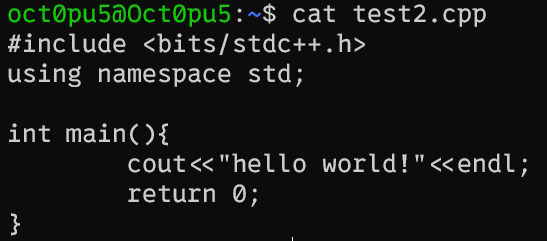
\includegraphics[width=0.9\textwidth,keepaspectratio]{assets/Linux/1.5 Linux file commands/2.png}
\end{figure}

\texttt{more} suits for files with a lot of content, which can be viewed
page by page instead of displaying everything like \texttt{cat}.

\begin{figure}[H]
    \centering
    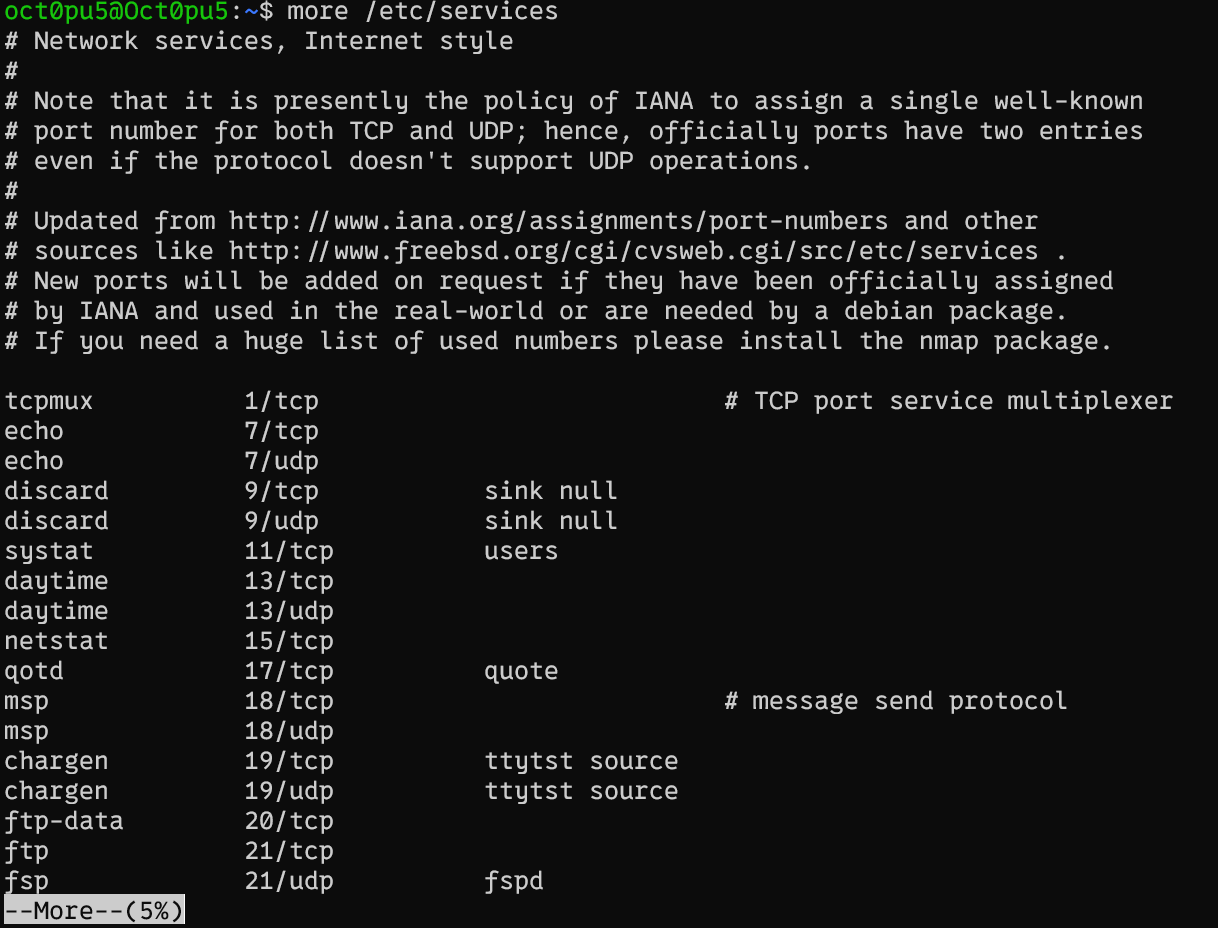
\includegraphics[width=0.9\textwidth,keepaspectratio]{assets/Linux/1.5 Linux file commands/3.png}
\end{figure}

\begin{mdquote}
Press \texttt{space} to turn the page, press \texttt{q} to quit.
\end{mdquote}

\subsubsection{\textbf{cp mv}}

\texttt{cp} copies files and folders from one path and pastes to another
path. Grammar here:
\texttt{cp\ {[}-r{]}\ \textless{}path1\textgreater{}\ \textless{}path2\textgreater{}}.

When \texttt{cp} a folder, \texttt{-r} is a must.

\begin{figure}[H]
    \centering
    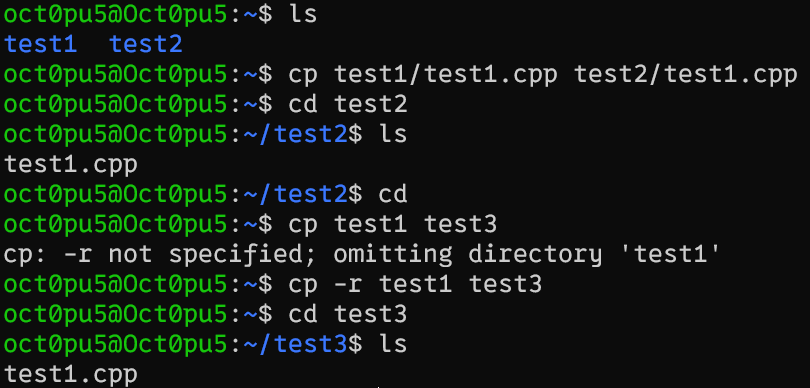
\includegraphics[width=0.75\textwidth,keepaspectratio]{assets/Linux/1.5 Linux file commands/4.png}
\end{figure}

\texttt{mv} moves files and folders from one path to another. Grammar
here:
\texttt{mv\ \textless{}path1\textgreater{}\ \textless{}path2\textgreater{}}.

\begin{figure}[H]
    \centering
    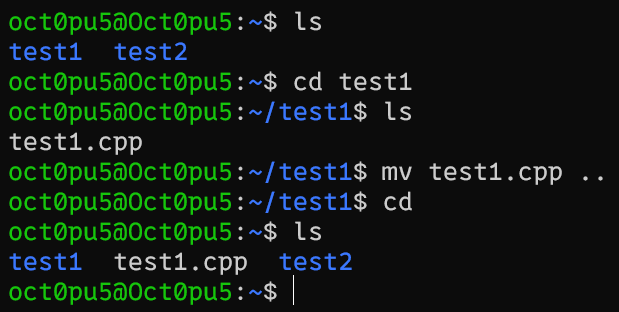
\includegraphics[width=0.9\textwidth,keepaspectratio]{assets/Linux/1.5 Linux file commands/5.png}
\end{figure}

\subsubsection{\textbf{rm}}

\texttt{rm} is a fantastic command. It deletes files and folders. Just
use
\texttt{rm\ -rf\ \textless{}file1\textgreater{}\ \textless{}file2\textgreater{}\ ...}\
to destroy your work. It can not only delete files and folders, but also
forcefully :)

OK. Don't be serious, I was joking. \texttt{rm}\ is a dangerous command.
According to Linux rules, it can delete \textbf{almost everything}. So I suggest
you to add \texttt{-i}\ parameter to confirm deletion. And don't use
\texttt{-f}\ (means forcefully) unless you are sure what you are doing.

\begin{mdquote}
If you don't want to input \texttt{-i}\ every time, you can add
\texttt{alias\ rm='rm\ -i'}\ to \texttt{.bashrc}. Then you get a
safer \texttt{rm}.
\end{mdquote}

I was keen on making my own virus when I was in high school. At that
time I write many viruses by \texttt{Visual\ Basic\ Scripts}\ such as
locking Desktop wallpaper or rebooting automatically. I also have a
point to delete files however I was confused by the complex user
permission system on Windows until now. When I met Linux, I knew my
dream come true.

\begin{mdquote}
Although this is just a joke (but it's damn fact),
listen to me my friends, \textbf{DON'T TRY THIS COMMAND
\texttt{sudo\ rm\ -rf\ /*}\ OR YOU WILL BE REGRETFUL!}
\end{mdquote}

\begin{figure}[H]
    \centering
    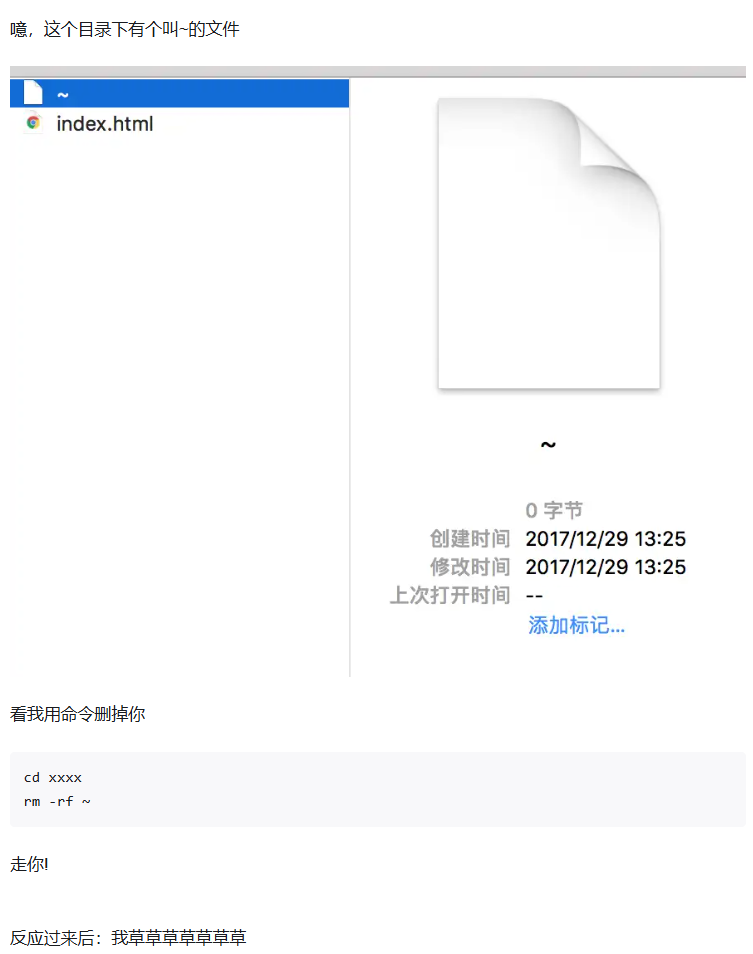
\includegraphics[width=0.8\textwidth,keepaspectratio]{assets/Linux/1.5 Linux file commands/6.png}
\end{figure}

This story tells us when you must use \texttt{rm}, be careful, think
twice and don't regret. And ask yourself a question, how
to delete this file properly?

\subsubsection{\textbf{which}}

\texttt{which} finds files called by commands. Grammar here:
\texttt{which\ {[}-a{]}\ \textless{}command\textgreater{}}.

\emph{P.S. \texttt{-a} is the most frequently used parameter, and I
ignored others.}

See the example below, It means \texttt{python3}\ and \texttt{g++}\ call
those 2 files.

\begin{figure}[H]
    \centering
    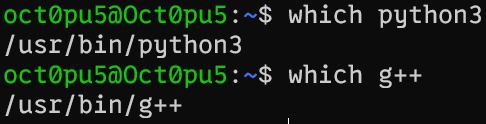
\includegraphics[width=0.9\textwidth,keepaspectratio]{assets/Linux/1.5 Linux file commands/7.png}
\end{figure}

\texttt{-a}\ is used to show all possible files. If you install Python
3.10.x and 3.11.x, you maybe need \texttt{which\ -a\ python3}.

\subsubsection{\textbf{find}}

\texttt{find}\ finds files based on file name or file size. Grammar here:
\texttt{find\ path\ -name\ 'name'} or
\texttt{find\ \textless{}path\textgreater{}\ -size\ +\textbar{}-n{[}k\ M\ G{]}}.


\begin{mdquote}
You should notice that \texttt{+}\ means \texttt{\textgreater{}}\ and
\texttt{-}\ means \texttt{\textless{}}\ when based on size. Also
\texttt{k}\ is a lowercase!*

\begin{figure}[H]
    \centering
    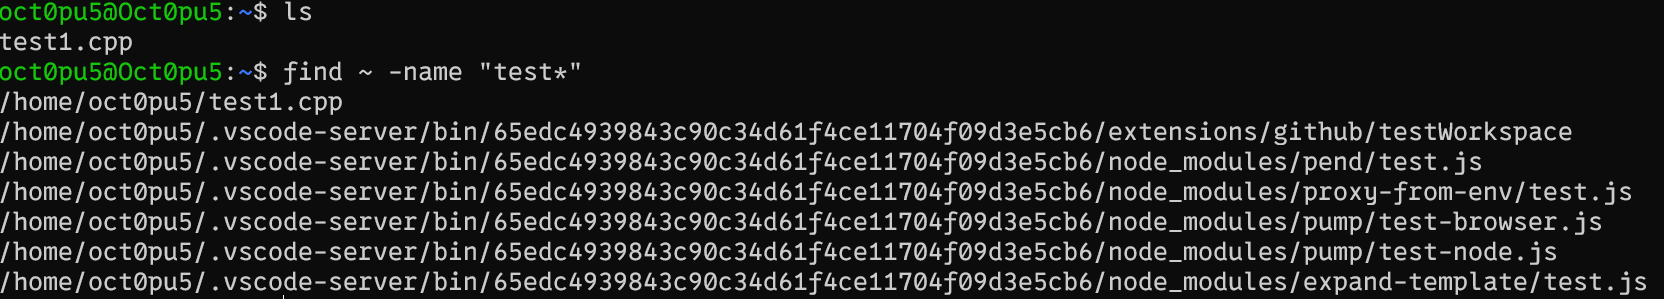
\includegraphics[width=0.9\textwidth,keepaspectratio]{assets/Linux/1.5 Linux file commands/8.png}
\end{figure}

\begin{figure}[H]
    \centering
    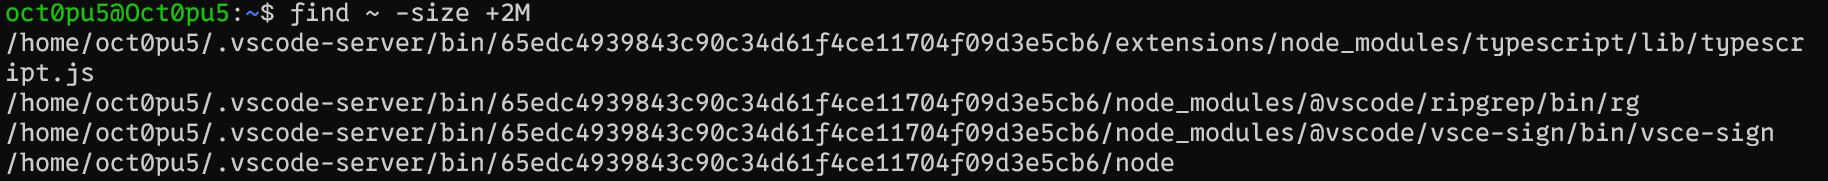
\includegraphics[width=0.9\textwidth,keepaspectratio]{assets/Linux/1.5 Linux file commands/9.png}
\end{figure}
\end{mdquote}

\subsubsection{\textbf{grep}}

\texttt{grep}\ is the same as \texttt{findstr}\ in Windows CMD. It can
filter string out. Grammar here:
\texttt{grep\ {[}-n{]}\ 'string'\ \textless{}path\textgreater{}}.

\begin{mdquote}
I suggest you always write \texttt{-n}\ because it shows which row it is.
\end{mdquote}

\begin{figure}[H]
    \centering
    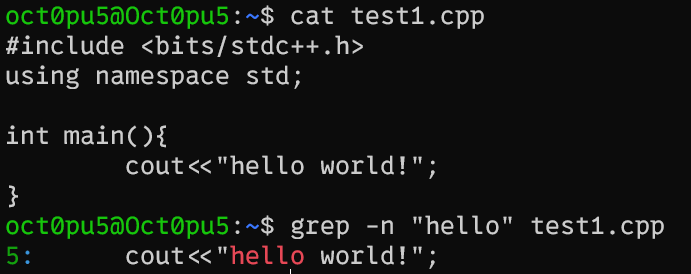
\includegraphics[width=0.9\textwidth,keepaspectratio]{assets/Linux/1.5 Linux file commands/10.png}
\end{figure}

Amazing, \texttt{grep}\ even give 'hello' a red color to emphasize.

After we learn \texttt{grep}, It is necessary to talk about a useful
symbol \texttt{\textbar{}}. We have known \texttt{\textbar{}\textbar{}}\
is \texttt{or}\ in C++. But this time we call \texttt{\textbar{}}\ pipe
symbol. It can connect 2 commands, and make the result of left command
be the input of right side. Here's an example:

\begin{figure}[H]
    \centering
    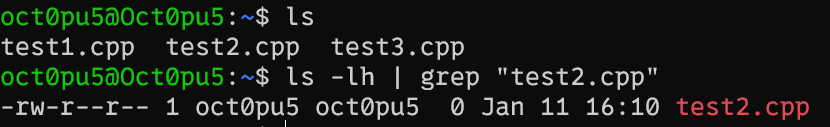
\includegraphics[width=0.9\textwidth,keepaspectratio]{assets/Linux/1.5 Linux file commands/11.png}
\end{figure}
\subsubsection{\textbf{wc}}

\texttt{wc}\ counts the rows, words, bytes, characters of a file. Grammar
here:\texttt{wc\ {[}-c\ -m\ -l\ -w{]}\ path}.

\begin{table}[H]
    \centering
    \begin{tabular}{cc}
    \toprule
    parameter & function \\
    \midrule
    \texttt{-c} & count bytes \\
    \texttt{-m} & count characters \\
    \texttt{-l} & count rows \\
    \texttt{-w} & count words \\
    \bottomrule
    \end{tabular}
\end{table}

If there isn't any parameter, \texttt{wc}\ will count
rows, words and bytes by default.

\begin{figure}[H]
    \centering
    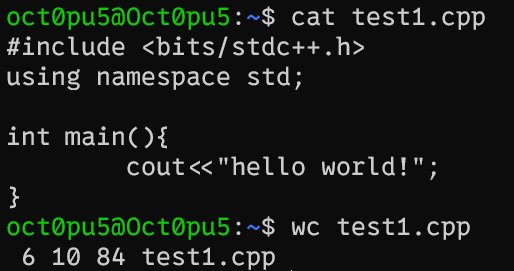
\includegraphics[width=0.9\textwidth,keepaspectratio]{assets/Linux/1.5 Linux file commands/12.png}
\end{figure}

\subsubsection{\textbf{echo}}

\texttt{echo}\ = \texttt{cout}, input \texttt{echo\ 'sth'}\ then terminal
returns sth.

If you think this section is over, it's completely
wrong. There are still some important symbols.

Have you met following experience, want to define a variable and
discover that it is a reserved word? What if I have to do like this? So
I introduce `` to encircle the reserved words. Example here:

\begin{figure}[H]
    \centering
    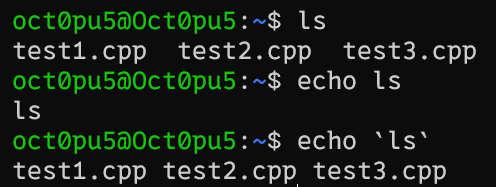
\includegraphics[width=0.9\textwidth,keepaspectratio]{assets/Linux/1.5 Linux file commands/13.png}
\end{figure}

Besides, if you have learnt Python data analysis, then you must know
file read and write operations.\ \texttt{echo}\ can also perform write
operations. In fact we just need 2 symbols to do our work.

\texttt{\textgreater{}}\ and \texttt{\textgreater{}\textgreater{}}\
connect a command and a file.

\texttt{\textgreater{}}\ overwrite the result of left command to the file
on the right side.

\texttt{\textgreater{}\textgreater{}}\ do the similar thing but actually
an append operation.

\begin{figure}[H]
    \centering
    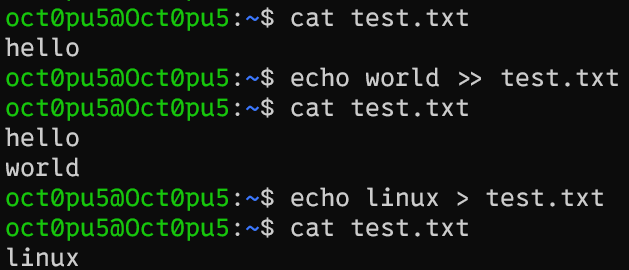
\includegraphics[width=0.9\textwidth,keepaspectratio]{assets/Linux/1.5 Linux file commands/14.png}
\end{figure}

\subsubsection{\textbf{tail}}

\texttt{tail}\ views the end of the file and also monitor the latest
changes to the file. Grammar here:
\texttt{tail\ {[}-f\ -num{]}\ \textless{}path\textgreater{}}.

\texttt{-num}\ means any number. For example, \texttt{-5}\ shows the last
5 rows of the file.

\texttt{-f}\ indicates the activation of monitoring. \texttt{tail}\ will
keep running, when the tracked file changes \texttt{tail}\ output the
changed content.

\begin{figure}[H]
    \centering
    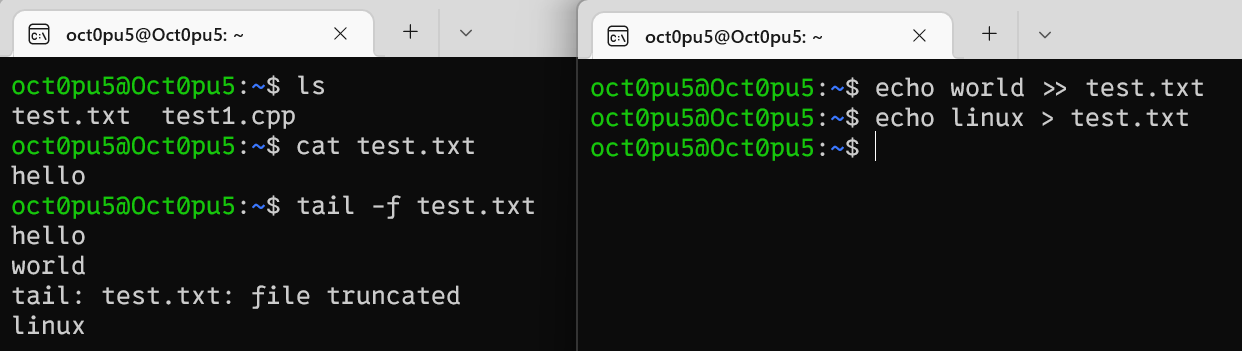
\includegraphics[width=0.9\textwidth,keepaspectratio]{assets/Linux/1.5 Linux file commands/15.png}
\end{figure}

When I input
\texttt{echo\ world\ \textgreater{}\textgreater{}\ test.txt}, left
terminal output \texttt{hello\ \textbackslash{}n\ world}. When I input
\texttt{\textgreater{}}\ which means overwrite, \texttt{tail}\ throw an
error. It told me \texttt{test.txt}\ is truncated. It tells us never
overwrite file or \texttt{tail}\ will be disabled. Moreover, there is
something troublesome below.

\begin{figure}[H]
    \centering
    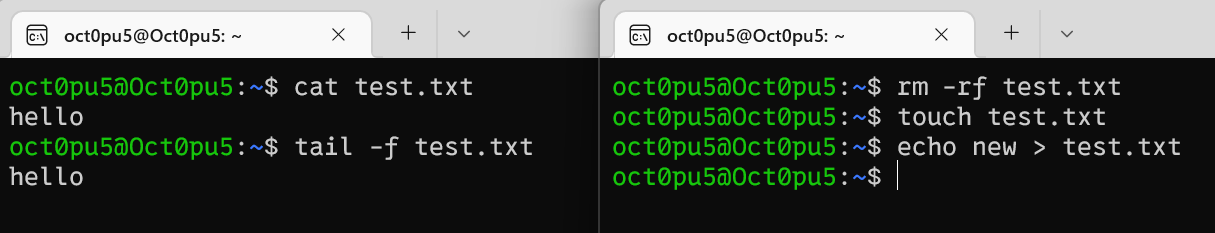
\includegraphics[width=0.9\textwidth,keepaspectratio]{assets/Linux/1.5 Linux file commands/16.png}
\end{figure}

I delete \texttt{test.txt}, and create a new one with a word 'new', but
\texttt{tail}\ have no output. How come?

Don't be worry, we have a solution: change \texttt{-f}\
to \texttt{-F}. Let's see what will happen.

\begin{figure}[H]
    \centering
    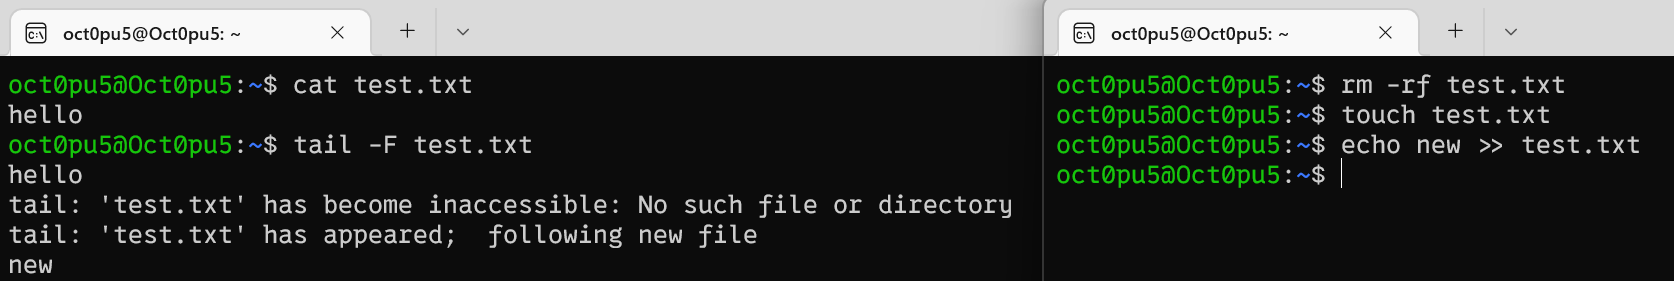
\includegraphics[width=0.9\textwidth,keepaspectratio]{assets/Linux/1.5 Linux file commands/17.png}
\end{figure}

Cool.\ \texttt{-F}\ will show hints when tracked file is deleted or
create.

\newpage
\subsection{\textbf{Linux user and permission commands}}
\begin{mdquote}
All commands in this chapter except \texttt{su}\ need \texttt{sudo}!
\end{mdquote}

\subsubsection{\textbf{Permission information}}

There are 3 permissions on Linux: \texttt{r}\ for read, \texttt{w}\ for
write and \texttt{x}\ for execute.

For a file or a folder, it carries permission information up to 10
characters long.The first character indicates this is a file \texttt{-},
a folder \texttt{d}\ or a soft link \texttt{l}. The remaining 9
characters are divided every 3 into a group. These 3 groups represent
user permissions, user group permissions, and other user permissions,
respectively.

Let's take an example. \texttt{drwxr-xr-x}\ means a
folder which current user can \texttt{rwx}\ and user group and other
users can only \texttt{r-x}.

\subsubsection*{\textbf{root}}

\texttt{root}\ user dominates Linux as \texttt{TrustedInstaller}\ on
Windows. And ordinary users can only control \texttt{/home}\ and
\texttt{r-x}\ the other directories.

\subsubsection*{\textbf{su}}

\textbf{S}witch \textbf{u}ser. Grammar here:
\texttt{su\ -\ {[}username{]}}. \texttt{-}\ is optional in fact, but I
recommend you to write it. If no \texttt{username}, \texttt{su\ -}\
switches to \texttt{root}\ by default.

Switching to \texttt{root}\ user needs password. It is entered by the
user themselves when creating the system, so please
don't ask others because they don't know
your password neither. If you really forget it, check \textbf{2.1 SHIT, 
I forgot my password again!}.

\begin{mdquote}
Don't always run commands as \texttt{root} user to save
efforts. It may cause unforeseen problems.
\end{mdquote}

To return to the user before switching, you can enter \texttt{exit}.

\subsubsection*{\textbf{sudo}}

We \textbf{STRONGLY}\ recommend everyone to use \texttt{sudo}\ rather than
\texttt{su\ -}\ in most situations. And it's easy, just
add \texttt{sudo}\ before commands that require permission, and it
requires password for the first time.

\begin{figure}[H]
    \centering
    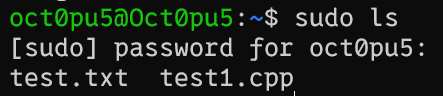
\includegraphics[width=0.9\textwidth,keepaspectratio]{assets/Linux/1.6 Linux user and permission commands/1.png}
\end{figure}

Linux is interesting. It won't display when typing
password. So recite your password, type it and press \texttt{Enter}.

\subsubsection{\textbf{user and user group}}

\subsubsection*{\textbf{user group}}

user must be in a user group. Try 2 commands below:
\texttt{groupadd\ \textless{}groupname\textgreater{}},
\texttt{groupdel\ \textless{}groupname\textgreater{}}.

\subsubsection*{\textbf{user}}

\texttt{useradd\ {[}-g\ -d{]}\ \textless{}username\textgreater{}}\ adds a
user.

\texttt{-g}\ appoints the user group. If no then creates a user group
with a same name automatically. If such a user group has already
existed, \texttt{-g}\ is a must.

\texttt{-d}\ appoints the \texttt{/home}\ path. If no then
\texttt{/home/username}\ by default.

\texttt{userdel\ {[}-r{]}\ \textless{}username\textgreater{}}\ deletes a
user.

\texttt{-r}\ deletes the \texttt{/home}\ path. If no then reserves it.

\texttt{id\ {[}username{]}}\ views the user group which the user belongs
to.

If no \texttt{username}\ then views the user itself who input this
command.

\texttt{usermod\ -aG\ \textless{}groupname\textgreater{}\ \textless{}username\textgreater{}}\
adds the user to the user group.

\texttt{getent\ passwd}\ views what the current users are. You can see me
in the end of the output.

\begin{figure}[H]
    \centering
    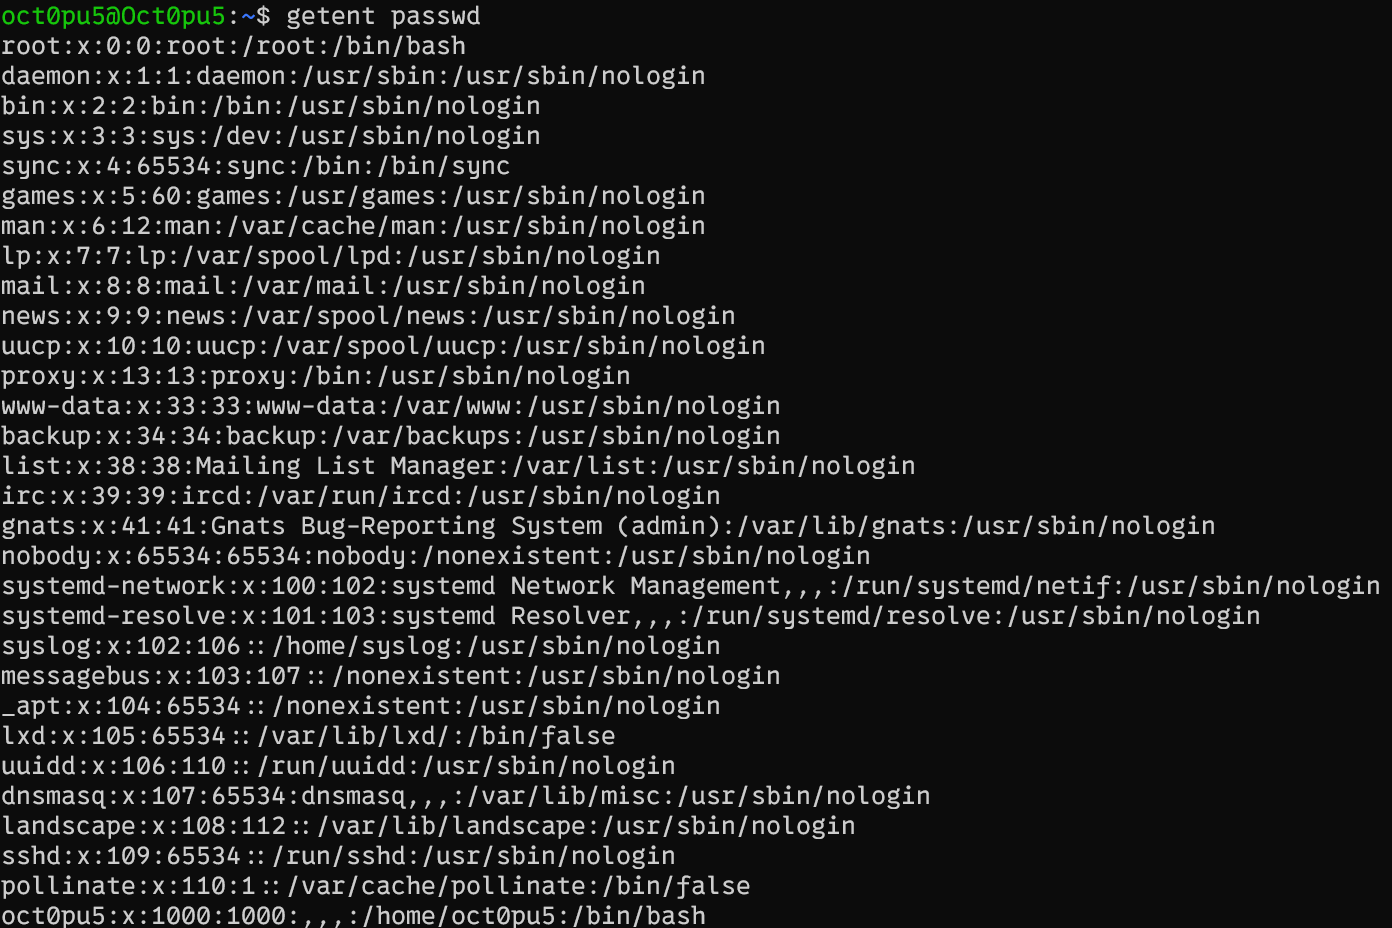
\includegraphics[width=0.9\textwidth,keepaspectratio]{assets/Linux/1.6 Linux user and permission commands/2.png}
\end{figure}

\texttt{getent\ group}\ views what the current groups are.

\subsubsection{\textbf{chmod}}

\texttt{chmod}\ changes files and folders permission. Grammar here:
`chmod {[}-R{]}.

\texttt{-R} refers to operating all files in the folder.

\texttt{permission}\ parameter has lots way to write. For example,
\texttt{u=rwx,\ g=rx,\ o=x}\ means \texttt{rwx}\ for user, \texttt{r-x}\
for user group and \texttt{-\/-x}\ for others.

Moreover, there is a method of using numbers to represent permissions,
which is very common. It sets \texttt{r}\ as 4, \texttt{w}\ as 2 and
\texttt{x}\ as 1 then creates 7 kinds of combination. Just remember 7
represents \texttt{rwx}\ and now we have a command
\texttt{chmod\ -R\ 777\ path}\ to achieve all permission of the file or
folder.

\subsubsection{\textbf{chown}}

\texttt{chown} changes user and user group to which file and folder
belong. Grammar here:
\texttt{chown\ {[}-R{]}\ {[}username{]}\ {[}:{]}\ {[}groupname{]}\ \textless{}path\textgreater{}}.

\texttt{-R}\ is the same as \texttt{chmod}. \texttt{{[}:{]}}\ split user
and user group.

Not very useful in my opinion :/

\subsection{\textbf{Tricks for a real Linuxer}}

\subsubsection{clear}

Sometimes the terminal looks really messy and you cannot find the
information you need at a glance. Now we have \texttt{clear}\ to bring a
clean screen back. It proves effective every time!

\begin{figure}[H]
    \centering
    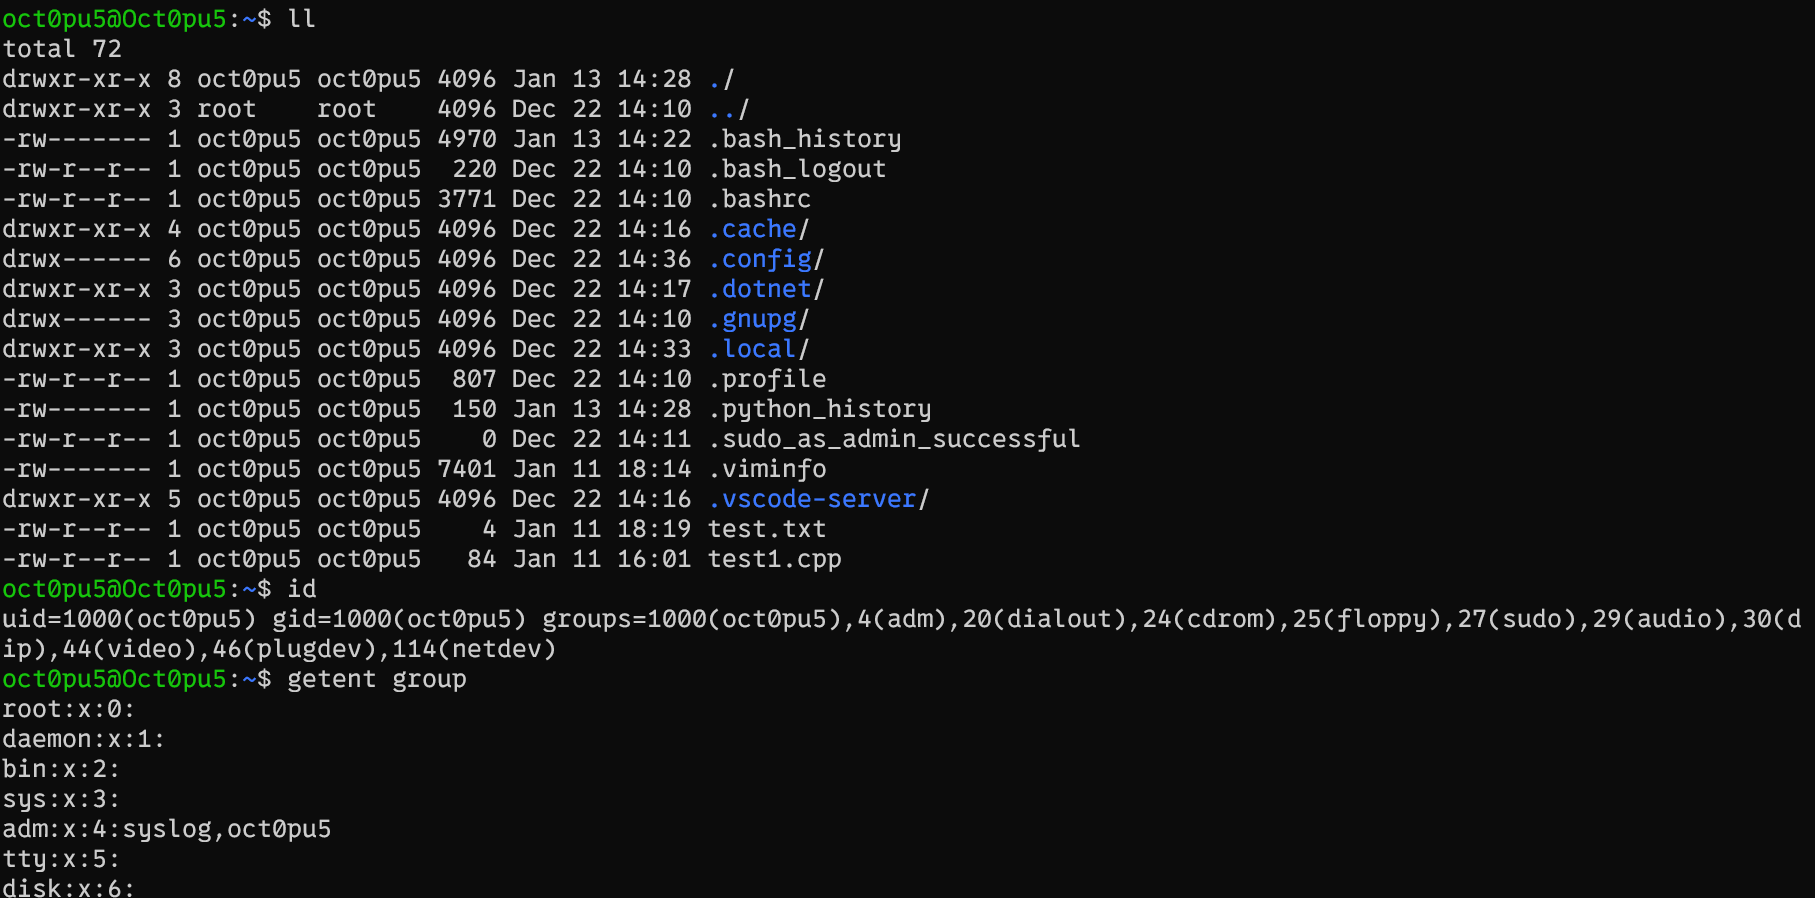
\includegraphics[width=0.9\textwidth,keepaspectratio]{assets/Linux/1.7 Tricks for a real Linuxer/1.png}
\end{figure}

\begin{mdquote}
More than that, \texttt{Ctrl+l}\ is the same as \texttt{clear}.
\end{mdquote}

\subsubsection{\texttt{tab}}

\begin{figure}[H]
    \centering
    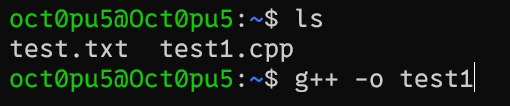
\includegraphics[width=0.9\textwidth,keepaspectratio]{assets/Linux/1.7 Tricks for a real Linuxer/2.png}
\end{figure}

I should input \texttt{test1.cpp}\ normally but if I press \texttt{tab}\
terminal will help me complete it automatically.\ \texttt{tab}\ do save
plenty of time when you have to input some long commands.

\subsubsection{\textbf{Search for commands with \texttt{↑}\ and
\texttt{↓}}}


\begin{figure}[H]
    \centering
    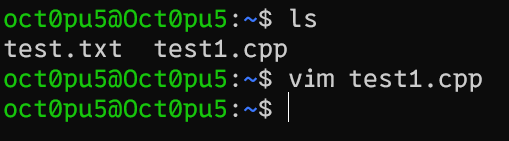
\includegraphics[width=0.9\textwidth,keepaspectratio]{assets/Linux/1.7 Tricks for a real Linuxer/3.png}
\end{figure}

I \texttt{vim\ test1.cpp}, what if I find a mistake? I have to type this
command again, too troublesome. But if I press \texttt{↑}, it will
appear directly.\ \texttt{↑}\ and \texttt{↓}\ is a quick way to search
history. I will introduce more in the following section
\textbf{history}.

\subsubsection{\textbf{history}}

Want to view previous commands? Feel slow for \texttt{↑}\ and \texttt{↓}?
\texttt{history}\ is capable of this task. In most situation we only need
\texttt{history\ num}\ and \texttt{num}\ is the number of commands you
want to view.

\begin{figure}[H]
    \centering
    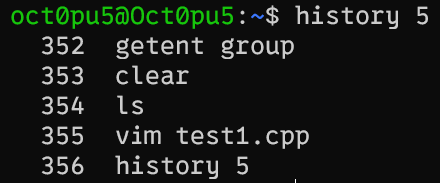
\includegraphics[width=0.9\textwidth,keepaspectratio]{assets/Linux/1.7 Tricks for a real Linuxer/4.png}
\end{figure}

\subsubsection{\textbf{ll}}

Do you feel inconvenient when inputting \texttt{ls\ -l}? Linux gives us
an upgrade plan \texttt{ll}.\ \texttt{ll}\ equals to \texttt{ls\ -l}\ and
it's shorter to type.

Also you can try \texttt{ll\ -h}\ which is the same as \texttt{ls\ -lh}.

\begin{figure}[H]
    \centering
    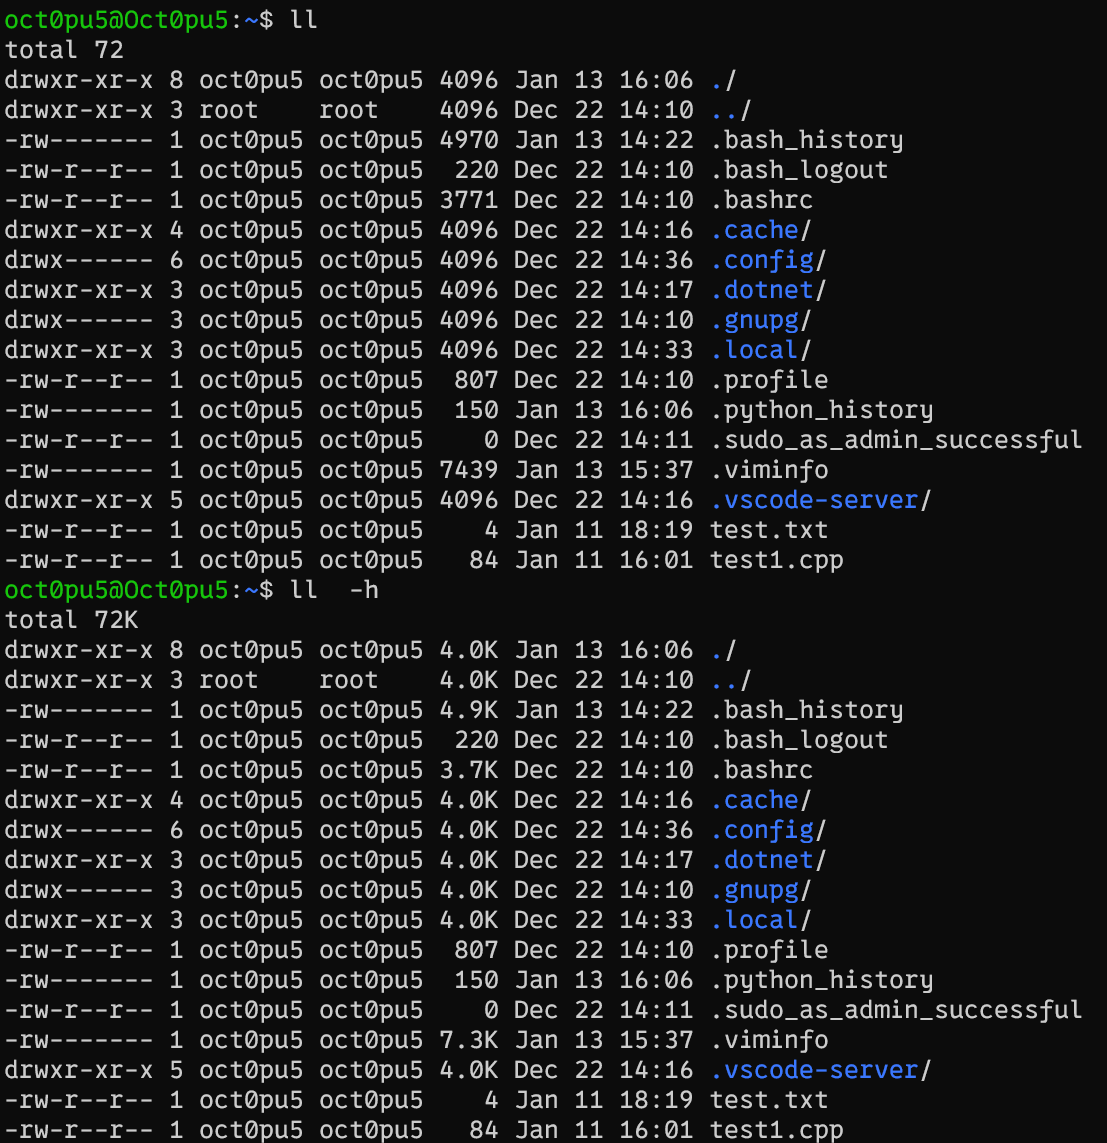
\includegraphics[width=0.9\textwidth,keepaspectratio]{assets/Linux/1.7 Tricks for a real Linuxer/5.png}
\end{figure}

\subsubsection{\textbf{\texttt{Ctrl}\ combination
keys}}

\subsubsection*{\textbf{\texttt{Ctrl+C}}}

Always remember \texttt{Ctrl+C}\ is NOT copy on Linux. It is a
\texttt{key\ interruption}\ to kill the process.

A simple example is, when you want to delete the database and resign you
need \texttt{sudo\ rm\ -rf\ /*}. What if you suddenly change your mind
during the process? \emph{Damn I must kill it RIGHT NOW!} Then
\texttt{Ctrl+C}\ helps you to save those poor remaining files. But
shouldn't be able to save your career.

\subsubsection*{\textbf{\texttt{Ctrl+Z}}}

Many confuse \texttt{Ctrl+Z}\ and \texttt{Ctrl+C}, regard them as the
same but actually not.\ \texttt{Ctrl+Z}\ freezes, or suspends the process.
That is to say you can restore this process, using \texttt{fg}.

\begin{figure}[H]
    \centering
    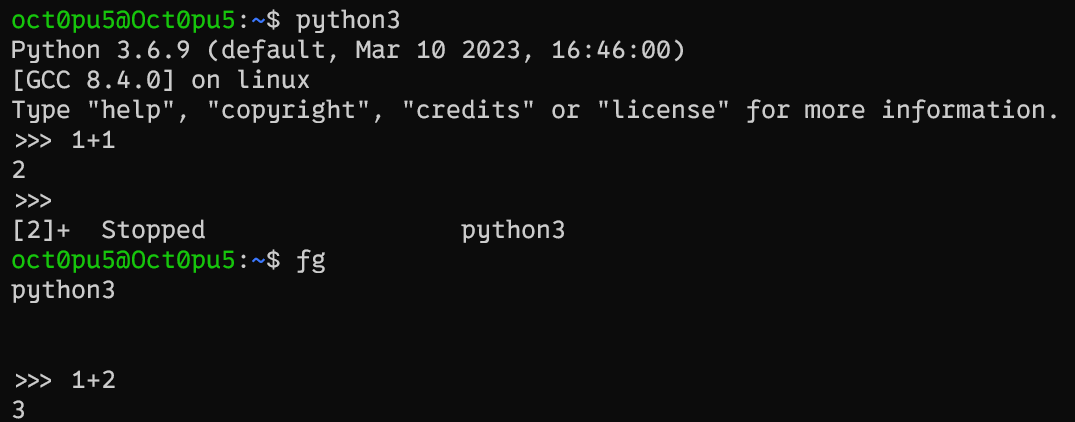
\includegraphics[width=0.9\textwidth,keepaspectratio]{assets/Linux/1.7 Tricks for a real Linuxer/6.png}
\end{figure}

In the figure above, we suspend \texttt{python3}\ with \texttt{Ctrl+Z}\
then restore it with \texttt{fg}. If it is \texttt{Ctrl+C}\
\texttt{python3}\ will be killed.

\subsubsection*{\textbf{\texttt{Ctrl+D}}}

\texttt{Ctrl+D}\ exits some status. We often use it to exit \texttt{root}\
user or compilers.

\begin{figure}[H]
    \centering
    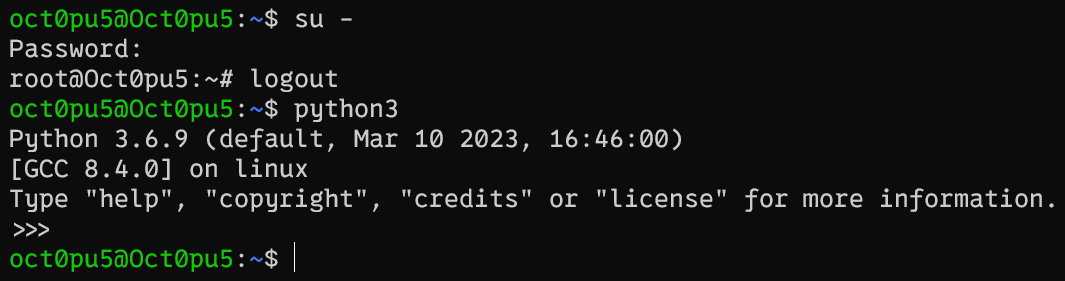
\includegraphics[width=0.9\textwidth,keepaspectratio]{assets/Linux/1.7 Tricks for a real Linuxer/7.png}
\end{figure}

I input \texttt{Ctrl+D}\ after \texttt{su\ -}\ and \texttt{python3}. Quite
convenient.

\subsubsection*{\textbf{\texttt{Ctrl+A / Ctrl+E}}}

\texttt{Ctrl+A}\ moves the cursor to the beginning of the row, and
\texttt{Ctrl+E}\ the end. They save time to click the mouse or hold
\texttt{←}\ and \texttt{→}.

\subsubsection*{\textbf{\texttt{Ctrl+S / Ctrl+Q}}}

Always remember \texttt{Ctrl+S}\ is NOT save on Linux. (I said familiar
words in the section \texttt{Ctrl+C}) It freezes the terminal. And
\texttt{Ctrl+Q}\ unfreezes.

What can they be used for? If you \texttt{tail\ -F}\ a file and a large
amount of text is written suddenly, to investigate the specific content,
you will freeze the terminal first. After you figure it out, unfreeze it
and continue to observe the following situation. So we can say
\texttt{Ctrl+S}\ and \texttt{Ctrl+Q}\ helps look through the content
displayed on terminal.

\newpage
\subsection{\textbf{Some trivial contents on Linux}}

\subsubsection{\textbf{Installing softwares}}

\begin{mdquote}
It has differences between Debian and CentOS in this section!
\end{mdquote}

Why Linux is hard to a newbie? I think it has a lot to do with the
hassle of installing softwares. On Windows, users open Microsoft Store
or Google Chrome, click 'Download' button and run the \texttt{.exe}\ at
most. But it seems quite troublesome on Linux. Though many softwares
provide \texttt{.deb}\ or other forms of installing packages on their
website, most people ignore them. That's a pity.

But don't worry, we can still install using our
terminal.

Next, I will take Debian as an example because CentOS has stopped
maintenance and there may be unforeseen problems.

\texttt{apt(-get)\ {[}install\ \textbar{}\ remove\ \textbar{}\ search{]}\ \textless{}name\textgreater{}}
helps install or uninstall softwares. Also it needs \texttt{root}\
permission so we add \texttt{sudo}.

Some software dependency libraries have been updated, but the software
dependency list has not been updated. Then you need to download a single
package. Use \texttt{wget\ url}. I will provide a more detailed
explanation in \textbf{1.9 Network commands on Linux}.


\begin{figure}[H]
    \centering
    \includegraphics[width=0.9\textwidth,keepaspectratio]{assets/Linux/1.8 Some trivial contents on Linux/1.png}
\end{figure}

\subsubsection{\textbf{Soft link}}

A soft link on Linux is like a shortcut on Windows. Grammar here:
\texttt{ln\ -s\ src\ dest}.

\begin{figure}[H]
    \centering
    \includegraphics[width=0.9\textwidth,keepaspectratio]{assets/Linux/1.8 Some trivial contents on Linux/2.png}
\end{figure}

\subsubsection{\textbf{date}}

\texttt{date} views system time. Grammar here:
\texttt{date\ {[}-d{]}\ \ {[}+format{]}}.

\texttt{-d}\ is used to calculate time, not very useful in my opinion.

Remember \texttt{+format}\ needs quotation marks when there is a space.
Here's a form including all time formats:

\begin{table}[H]
    \centering
    \begin{tabular}{cc}
    \toprule
    format & meaning \\
    \midrule
    \%Y & year \\
    \%y & the last 2 numbers of the year \\
    \%m & month \\
    \%d & day \\
    \%H & hour \\
    \%M & minute \\
    \%S & second \\
    \bottomrule
    \end{tabular}
\end{table}

\begin{figure}[H]
    \centering
    \includegraphics[width=0.9\textwidth,keepaspectratio]{assets/Linux/1.8 Some trivial contents on Linux/3.png}
\end{figure}

\subsubsection{\textbf{File Descriptor and Redirection Operators}}

\begin{mdquote}
Check this blog for more information: \url{https://www.cnblogs.com/hls-code/p/16968319.html}.
\end{mdquote}

\subsubsection*{\textbf{File Descriptor}}

A file descriptor is an integer associated with the input and output of a file.
The most 3 common are \texttt{stdin},\ \texttt{stdout}\ and \texttt{stderr}. 
They are 0, 1 and 2 respectively.

\texttt{stdin}\ is the standard input, which is what you type in the terminal.
\texttt{stdout}\ is the standard output, which is what you see in the terminal.
\texttt{stderr}\ is the standard error, which is the error message you see in the terminal.

\subsubsection*{\textbf{Redirection Operators}}

If you still remember what I said in \textbf{1.5 Linux file commands},
you can use \texttt{>}\ and \texttt{>>}\ to redirect the output of a command to a file.
They are the redirection operators. Redirection operators are using file descriptors.
For example, \texttt{>}\ is the same as \texttt{1>}. Then you must know what \texttt{2>}\ means:
It redirects the error message to a file.

Here is a advanced usage.\ \texttt{2\textgreater{}\&1}\ means redirecting the error message
to the standard output. It is often used to save errors to a log with the standard output.

\begin{mdquote}
This is a very useful skill!
\end{mdquote}

Moreover, \texttt{<}\ reads the content of a file as the input of a command,
and \texttt{<<}\ reads the content of a file as the input of a command until a delimiter.

\subsection*{\texttt{/dev/null}}

\texttt{/dev/null} is a special file that discards all data written to it so we
call it the black hole. It's useful when you want to discard error messages to
make the output more clear. Here's an example:

\begin{figure}
    \centering
    \includegraphics[width=0.9\textwidth,keepaspectratio]{assets/Linux/1.8 Some trivial contents on Linux/4.png}
\end{figure}

\texttt{cat /dev/null > test.cpp}\ is just the same as \texttt{echo "" > test.cpp}.
It cleans the file but doesn't delete it.

\begin{mdquote}
\texttt{bash} will popup an error when you want to \texttt{>}\ an existing file by default.
You can input \texttt{set\ +o\ noclobber}\ to disable this function. But \textbf{remember to enable
it by \texttt{set\ -o\ noclobber}\ after testing!}
\end{mdquote}

\subsection{\textbf{Network commands on Linux}}

\subsubsection{\textbf{hostname and IP}}

IP is your network address if you are connected to the internet.
It's divided into IPv4 and IPv6. Our country use IPv4
more often from a data perspective. Hostname is the OS name. Others on
the internet find you by your IP and hostname.

Input \texttt{ifconfig}\ and the terminal shows lots of information. Pay
attention to \texttt{eth0}, you will find \texttt{inet}, the following
is IP.

\begin{figure}[H]
    \centering
    \includegraphics[width=0.9\textwidth,keepaspectratio]{assets/Linux/1.9 Linux network commands/1.png}
\end{figure}

Input \texttt{hostname}\ to check your hostname. Or
there's an easier way, your hostname is behind '@' on
the terminal.

If you aren't satisfied with this name.\emph{When did I
come up with such a reckless name!}\ Don't worry, you can
certainly change it.
\texttt{hostnamectl\ set-hostname\ \textless{}name\textgreater{}}\ saves
your young soul. Like this:

\begin{figure}[H]
    \centering
    \includegraphics[width=0.9\textwidth,keepaspectratio]{assets/Linux/1.9 Linux network commands/2.png}
\end{figure}

\subsubsection{\textbf{ping}}

\texttt{ping} checks whether the server is connectable. Grammar here:
\texttt{ping\ {[}-c\ num{]}\ \textless{}ip/hostname\textgreater{}}.

\texttt{-c\ num} decides how many times you \texttt{ping}. If no then
infinite.

\begin{figure}[H]
    \centering
    \includegraphics[width=0.9\textwidth,keepaspectratio]{assets/Linux/1.9 Linux network commands/3.png}
\end{figure}

\texttt{ping}\ can not only determine if the server is functioning
properly, but also you are connected to the internet. Obviously you
won't \texttt{ping}\ anything when offline.

\subsubsection{\textbf{wget}}

\texttt{wget} is a powerful command to download things from the
internet. It has many parameters that can't be omitted
into a sentence. However, we can talk about a few of the most commonly
used ones.

\texttt{-O}\ renames files you download. Like this:
\texttt{wget\ oct0pu5.cn\ -O\ oct0pu5.html}.

\texttt{-i}\ makes \texttt{wget}\ can download multiple files like
\texttt{pip\ install\ -r}. Make a \texttt{requirements.txt}\ if is
needed, and input \texttt{wget\ -i\ requirements.txt}.

When the file is very large, it spends a long time. Also, Linux maybe
throw errors during transmission. We can add \texttt{-b}\ to download in
the background and \texttt{-c}\ to achieve file breakpoint resume. Now I
will explain both separately.

\texttt{wget\ -b\ url}\ are used together with \texttt{tail\ -F}\
generally.\ \texttt{wget-log}\ shows the progress. In this example
\texttt{index.html}\ is downloaded in the blink of a eye so
\texttt{wget-log}\ is empty.

\begin{figure}[H]
    \centering
    \includegraphics[width=0.9\textwidth,keepaspectratio]{assets/Linux/1.9 Linux network commands/4.png}
\end{figure}

\texttt{wget\ -c\ {[}-t\ num{]}\ {[}-T\ num{]}\ url}\ avoids the issue of
file download interruption.\ \texttt{-t\ num}\ is the times of retry. If
no then infinite.\ \texttt{-T\ num}\ is timeout waiting time.
\texttt{wget}\ will retry if timeout waiting time is exceeded.

\subsubsection{\textbf{curl}}

\begin{mdquote}
Debian may require self installation of \texttt{curl}. Input
\texttt{sudo\ apt\ install\ curl}.
\end{mdquote}

\texttt{curl}\ send a web request. Grammar here:
\texttt{curl\ {[}-O\ \textbar{}\ -o\ rename{]}\ \textless{}url\textgreater{}}.

\texttt{-O}\ is a must if downloading files.\ \texttt{-o}\ renames the
file.

I have to say again that the main function of \texttt{curl}\ is sending
web requests, downloading files is just a part. So I suggest you to use
\texttt{wget}\ more currently.

\subsubsection{\textbf{Port}}

Port is the interface for computer interaction. Our familiar USB, VGA
are all physical ports. And we also have virtual ports in computer OS.
Linux has 65536 ports. They are 0 to 65535 and divided into 3 parts.

\begin{table}[H]
    \centering
    \begin{tabular}{cc}
    \toprule
    port number & usage \\
    \midrule
    0--1023 & Called by system built-in services \\
    1024--49151 & Users can call freely \\
    49152--65535 & Used for temporary network connection calls \\
    \bottomrule
    \end{tabular}
\end{table}

\subsubsection*{\textbf{netstat}}

\texttt{netstat}\ can check the port occupancy status. Use
\texttt{netstat\ -tunpl}\ to show all information you need. Prototype,
local address, ports, states and PID, everything is in sight.

\begin{figure}[H]
    \centering
    \includegraphics[width=0.9\textwidth,keepaspectratio]{assets/Linux/1.9 Linux network commands/5.png}
\end{figure}

\subsection{\textbf{Linux process commands}}

\subsubsection{\textbf{Process}}

Applications are managed by OS. OS registers process for a running
application and a unique PID for every process.

\subsubsection{\textbf{ps}}

\texttt{ps\ -ef}\ shows all information of all process.

\begin{figure}[H]
    \centering
    \includegraphics[width=0.9\textwidth,keepaspectratio]{assets/Linux/1.10 Linux process commands/1.png}
\end{figure}

\texttt{UID}\ is the user to which the process belongs.\ \texttt{PPD}\ is
the \texttt{PID}\ of parent process.\ \texttt{C}\ is CPU usage.
\texttt{STIME}\ is the start time.\ \texttt{TTY}\ is the number of start
terminal, if not terminal startup then '?'.\ \texttt{TIME}\ is the time
that process occupies CPU.\ \texttt{CMD}\ is the path or commands.

\subsubsection{\textbf{pstree}}

\texttt{pstree}\ is more like an upgraded version of \texttt{ps}. It
shows process in a tree structure.

\begin{figure}[H]
    \centering
    \includegraphics[width=0.9\textwidth,keepaspectratio]{assets/Linux/1.10 Linux process commands/2.png}
\end{figure}

You can see the \texttt{pstree}\ is controlled by \texttt{bash}.

\subsubsection{\textbf{kill}}

\texttt{kill}\ closes the process. Grammar here:
\texttt{kill\ {[}-9{]}\ \textless{}PID\textgreater{}}.

\texttt{-9}\ means close forcefully (or kill).

\texttt{kill}\ is usually used together with \texttt{ps}. See this
example:

\begin{figure}[H]
    \centering
    \includegraphics[width=0.9\textwidth,keepaspectratio]{assets/Linux/1.10 Linux process commands/3.png}
\end{figure}

I \texttt{tail\ -F}\ a file and \texttt{kill}\ it. It shows 'Terminated'
which means it closes itself. And when \texttt{kill\ -9}\ 'Killed' means
OS closes it forcefully.

\subsubsection{\textbf{top}}

\texttt{top}\ monitors process information in real-time. \texttt{top}\
refreshes every 3 seconds by default. We usually use \texttt{top\ -i}\ to
ignore those inactive process.

\begin{figure}[H]
    \centering
    \includegraphics[width=0.9\textwidth,keepaspectratio]{assets/Linux/1.10 Linux process commands/4.png}
\end{figure}

Look, I am \texttt{vim}-ing a file. And there're more
left.

First row, \texttt{top}\ shows OS time, how long the OS has run, how many
users have logged in and \texttt{load\ average}\ is system load in 1, 5
and 15 minutes.

Second, how many tasks, how many of them are running, sleeping, have
stopped or are zombie process.

Third, \texttt{\%CPU(s)}\ is CPU usage.\ \texttt{us}\ is user CPU usage.
\texttt{sy} is system CPU usage.\ \texttt{ni}\ is the ratio of CPU time
occupied by high priority processes.\ \texttt{id}\ is free CPU usage.
\texttt{wa}\ is I/O waiting CPU usage.\ \texttt{hi}\ is CPU hardware
interrupt rate.\ \texttt{si}\ is CPU software interrupt rate.\ \texttt{st}\
is forcefully waiting CPU usage.

Fourth and fifth,\ \texttt{Mem}\ is physical RAM and \texttt{Swap}\ is
virtual RAM.

Continuing downwards, there is a row of headers.\ \texttt{PR}\ is the
priority, the smaller the higher.\ \texttt{NI}\ is also the priority,
positive represents low, 0 represents medium and negative represents
high.\ \texttt{VIRT},\ \texttt{RES}\ and \texttt{SHR} represent virtual,
physical and shared memory.\ \texttt{S}\ is process status.\ \texttt{S},\
\texttt{R},\ \texttt{Z},\ \texttt{N},\ \texttt{I} is sleeping, running,
zombie, low priority and idle.\ \texttt{\%CPU}\ and \texttt{\%MEM}\ is CPU
and memory usage.\ \texttt{TIME+}\ is the time that process occupies CPU.

\newpage
\subsection{\textbf{Linux environment variables}}

\subsubsection{\textbf{Environment variable}}

Environment variables are parameters which specify OS runtime
environment. It counts a lot and is usually global. A common example is
that the installer asks if add environment variables automatically when
you are installing Python. If there are no environment variables, Python
can't find most of its libraries. In other words, how
could it work!

\subsubsection{\textbf{env}}

\texttt{env} views all environment variables on Linux.

\begin{figure}[H]
    \centering
    \includegraphics[width=0.9\textwidth,keepaspectratio]{assets/Linux/1.11 Linux environment variables/1.png}
\end{figure}

I only showed a part of it. There are some points we should understand.

\texttt{USER}\ is current user.\ \texttt{PWD}\ is current directory.
\texttt{HOME}\ is current user's \texttt{/home}.
\texttt{PATH}\ contains directories of all executable files.

\subsubsection{\textbf{\$}}

\texttt{\$}\ represents taking variable values. When characters are
connected together, \texttt{\{\}}\ needs to be added. Like this:

\begin{figure}[H]
    \centering
    \includegraphics[width=0.9\textwidth,keepaspectratio]{assets/Linux/1.11 Linux environment variables/2.png}
\end{figure}

\subsubsection{\textbf{Add environment variables}}

There are many ways to add environment variables, including temporary
and permanent ones.

\texttt{export\ var=\textless{}value\textgreater{}}\ temporarily adds a
environment variable. It is only valid in the current terminal.

\begin{figure}[H]
    \centering
    \includegraphics[width=0.9\textwidth,keepaspectratio]{assets/Linux/1.11 Linux environment variables/3.png}
\end{figure}

And 2 ways to add permanently. Write \texttt{\textasciitilde{}/.bashrc}\
for current user or \texttt{/etc/profile}\ for all users. Then run
\texttt{source\ thatfile} to make it effective.

\begin{figure}[H]
    \centering
    \includegraphics[width=0.9\textwidth,keepaspectratio]{assets/Linux/1.11 Linux environment variables/4.png}
\end{figure}

\begin{figure}[H]
    \centering
    \includegraphics[width=0.9\textwidth,keepaspectratio]{assets/Linux/1.11 Linux environment variables/5.png}
\end{figure}

By the way, you can see codes below in \texttt{.bashrc}:

\begin{figure}[H]
    \centering
    \includegraphics[width=0.9\textwidth,keepaspectratio]{assets/Linux/1.11 Linux environment variables/6.png}
\end{figure}

You can input \texttt{ls\ -\/-help}\ for more information about
\texttt{ls}, and also write
\texttt{alias\ lh='ll\ -h'}\ to create
your own commands.

\newpage
\subsection{\textbf{Linux compression commands}}

\subsubsection{\textbf{Murmurs}}

I personally feel that compression and decompression related commands
are one of the most troublesome contents in this tutorial. But we still
have to overcome difficulties. There is a good news that this chapter is
the end of the main part of the tutorial (but not the end of your Linux
learning road :D). I know you must be tired but cheer up!

\subsubsection{\textbf{tar}}

Before the commands, let's understand the types of
compressed files on Linux first.\ \texttt{.zip}\ is the same as Windows,
but not the most common.\ \texttt{.tar}\ and \texttt{.tar.gz}\ are created
by \texttt{tar}\ and \texttt{gzip}.\ \textbf{They are the most commonly
used form.}

But wait, do you think of a question. Why Windows prefers \texttt{zip}\
but Linux not? Why not the two OSs unify compression format?

It's definitely a good question. Linux allows
\texttt{.zip}\ or \texttt{.7z}\ without problems. But they have a fatal
disadvantage that they CANNOT storage Linux permission information (do
you still remember it?). Therefore, \texttt{tar}\ is irreplaceable in a
sense. Even the backend of \texttt{tar}\ can be changed to \texttt{zip}\
or \texttt{7z}, but they lose the battle with \texttt{tar}\ on Linux.

Now we can introduce our best friend \texttt{tar}\ formally. Strictly
speaking \texttt{tar}\ isn't a kind of compression, it
archives files in fact. \texttt{tar}\ puts files into a package without
too much compression. The true implementation of compression or
decompression is \texttt{gzip}. Moreover, \texttt{gzip}\ is also an
compression algorithm. In other words, we call this the backend of
\texttt{tar}.

\begin{mdquote}
There are more algorithm except \texttt{gzip}, but it's
commonly used.
\end{mdquote}

Here's the grammar:
\texttt{tar\ {[}-c\ \textbar{}\ -v\ \textbar{}\ -x\ \textbar{}\ -f\ \textbar{}\ -z\ \textbar{}\ -C{]}\ \textless{}file1\textgreater{}\ \textless{}file2\textgreater{}\ ...}.

\texttt{-c}\ is compression. On the contrary \texttt{-x}\ is
decompression.

\texttt{-v}\ shows the progress.

\texttt{-f}\ is followed by files, it's required in most
cases.

\texttt{-z}\ opens \texttt{gzip}\ mode which means it will create
\texttt{.tar.gz}.

\texttt{-C}\ changes the destination of decompression.

I recommend you to put \texttt{-z}\ at first (if there's
\texttt{-z}) and \texttt{-f}\ at last to avoid errors.

I compressed 3 c++ files and decompressed them into
\texttt{\textasciitilde{}/decompression}. Don't forget
to \texttt{mkdir}\ or it will throw error!


\begin{figure}[H]
    \centering
    \includegraphics[width=0.9\textwidth,keepaspectratio]{assets/Linux/1.12 Linux compression commands/1.png}
\end{figure}

There is a tip in the figure above.\ \texttt{-zcvf}\ can be decompressed
by \texttt{-xvf}\ and \texttt{-zxvf}, but \texttt{-cvf}\ can be only
decompressed by \texttt{-xvf}. It's easy to make
mistakes here. My suggestion is to compress everything in \texttt{gzip}\
format.

\subsubsection{\textbf{More to say}}

I was planning to talk about \texttt{zip}.\ \texttt{zip}\ is more familiar
to Windows users, but in order to avoid the bad habit of only using
\texttt{zip}, I decided not to introduce it. If you have to use it,
check this blog:
\url{https://blog.csdn.net/weixin_49114503/article/details/132812358}.
But remember, \texttt{zip}\ isn't easier than
\texttt{tar}.

After learning this chapter, you should know what it is.
Don't ask similar silly questions again.

\begin{figure}[H]
    \centering
    \includegraphics[width=0.9\textwidth,keepaspectratio]{assets/Linux/1.12 Linux compression commands/2.png}
\end{figure}

\newpage
\thispagestyle{empty}
\begin{center}
    \vspace*{96pt}
    \fontsize{60}{60}\customfont{2}\par
    \fontsize{26}{31.2}\section{\textbf{Advanced Usage}}\par % 标题
    \vspace{25pt}
    \fontsize{18}{21.6}\selectfont{\textit{Without absolute certainty, what do we do? We do the best we can. ---RMS}}\par % 名言
    \vfill
\end{center}

\fontsize{12}{14}
\newpage
\subsection{\textbf{SHIT, I forgot my password again!}}

\subsubsection{\textbf{WSL}}

This is one reason why I recommend WSL. Open \texttt{Powershell}\ or
\texttt{Windows\ Terminal}, input \texttt{wsl\ -u\ -root}. Ignore the
warnings (If there are) then WSL becomes active and you are the root
user. And \texttt{passwd\ \textless{}username\textgreater{}}\ helps a
lot.

\begin{figure}[H]
    \centering
    \includegraphics[width=0.9\textwidth,keepaspectratio]{assets/Linux/2.1 SHIT, I forgot my password again!/1.png}
\end{figure}

\subsubsection{\textbf{Not WSL?}}

\subsubsection*{\textbf{Terminal}}

If you still remember the password of your account, the problem will be
much simpler. Input \texttt{sudo\ passwd\ root}\ and the terminal will
ask password of the current user.

\begin{figure}[H]
    \centering
    \includegraphics[width=0.9\textwidth,keepaspectratio]{assets/Linux/2.1 SHIT, I forgot my password again!/2.png}
\end{figure}

But what if you even forget your own password? You want to
\texttt{su\ -}\ to reset your password and need your password to reset
root user password. This is trapped in a \texttt{while(1)}\ endless loop.
So we can only take out our last resort.

\subsubsection*{\textbf{GRUB}}

Take Ubuntu as an example. Boot Ubuntu and hold \texttt{shift}\ to enter
\texttt{GRUB}\ (like \texttt{BIOS}\ on Windows) menu. Select
\textbf{Advance options for Ubuntu.}

\begin{figure}[H]
    \centering
    \includegraphics[width=0.9\textwidth,keepaspectratio]{assets/Linux/2.1 SHIT, I forgot my password again!/3.png}
\end{figure}

Select \textbf{recovery mode}.

\begin{figure}[H]
    \centering
    \includegraphics[width=0.9\textwidth,keepaspectratio]{assets/Linux/2.1 SHIT, I forgot my password again!/4.png}
\end{figure}

Wait a second and select \textbf{Drop to root shell prompt}.

\begin{figure}[H]
    \centering
    \includegraphics[width=0.9\textwidth,keepaspectratio]{assets/Linux/2.1 SHIT, I forgot my password again!/5.png}
\end{figure}

Then \texttt{passwd}\ and input your new password. Ignore the error that
I accidentally pressed a \texttt{space}.

\begin{figure}[H]
    \centering
    \includegraphics[width=0.9\textwidth,keepaspectratio]{assets/Linux/2.1 SHIT, I forgot my password again!/6.png}
\end{figure}

After that, select \textbf{Resume normal boot}. You can use it normally
now.

\newpage
\subsection{\textbf{MobaXterm, go ssh it!}}

\begin{mdquote}
Check this blog for more detail:
\url{https://blog.csdn.net/erciguihua/article/details/144258751}.
\end{mdquote}

\subsubsection{\textbf{Before the beginning}}

\begin{mdquote}
Your Windows version must be at least Windows11 22H2. That means your
laptop is bought at least after June, 2023 or you must upgrade your
Windows.
\end{mdquote}

Create \texttt{.wslconfig}\ in
\texttt{C:\textbackslash{}Users\textbackslash{}\textless{}username\textgreater{}}\
on Windows. After that write codes below:

\begin{adjustwidth}{2em}{0pt}
\begin{verbatim}
[wsl2]
networkingMode=mirrored
dnsTunneling=true
firewall=true
autoProxy=true
[experimental]
autoMemoryReclaim=gradual
\end{verbatim}
\end{adjustwidth}

Also, Open the Powershell and try these 2 commands below. One of them is
effective.

\begin{verbatim}
    Set-NetFirewallHyperVVMSetting -Name 
    ‘{40E0AC32-46A5-438A-A0B2-2B479E8F2E90}' 
    -DefaultInboundAction Allow

    # or

    New-NetFirewallHyperVRule -Name MyWebServer 
    -DisplayName “My Web Server” -Direction Inbound 
    -VMCreatorId “{40E0AC32-46A5-438A-A0B2-2B479E8F2E90}”
    -Protocol TCP -LocalPorts 80
\end{verbatim}

It will not only solve problems such as \emph{WSL in NAT mode
doesn't support \texttt{localhost}\ proxy} and IP address
for WSL changes frequently.

For more information, check this blog:
\href{https://blog.csdn.net/2301\_81697902/article/details/137481359}{https://blog.csdn.net/2301\_81697902/article/details/137481359}.

\subsubsection{\textbf{Downloading and cracking}}

This is the official website: \href{https://mobaxterm.mobatek.net/}{https://mobaxterm.mobatek.net/} and
the Chinese version:
\url{https://github.com/RipplePiam/MobaXterm-Chinese-Simplified}. I take
the original version as an example.

\begin{figure}[H]
    \centering
    \includegraphics[width=0.85\textwidth,keepaspectratio]{assets/Linux/2.2 MobaXterm, go ssh it!/1.png}
\end{figure}

Next, we will start to generate a key to crack it. Check this
repository: \url{https://github.com/flygon2018/MobaXterm-keygen}.

Open it with your VSCode (If you don't have VSCode,
Pycharm is also ok). Create a new terminal in current path. Input
\texttt{Python\ MobaXterm-Keygen.py\ \textless{}username\textgreater{}\ \textless{}version\textgreater{}}\
then It will generate a \texttt{Custom.mxtpro}. Move it into MobaXterm
folder and it's done.

\texttt{username}\ can be named arbitrarily and \texttt{version}\ is up to
your MobaXterm version.

\begin{figure}[H]
    \centering
    \includegraphics[width=0.85\textwidth,keepaspectratio]{assets/Linux/2.2 MobaXterm, go ssh it!/2.png}
\end{figure}

And you can open MobaXterm and click \texttt{About}\ to check it.

\begin{figure}[H]
    \centering
    \includegraphics[width=0.85\textwidth,keepaspectratio]{assets/Linux/2.2 MobaXterm, go ssh it!/3.png}
\end{figure}

\subsubsection{\textbf{Usage}}

Open \texttt{Session}\ and choose \texttt{WSL}. Change
\texttt{Distribution}\ to \texttt{Debian}. Then you can connect to WSL by
MobaXterm.

\begin{figure}[H]
    \centering
    \includegraphics[width=0.85\textwidth,keepaspectratio]{assets/Linux/2.2 MobaXterm, go ssh it!/4.png}
\end{figure}

Left side is a \texttt{SFTP}\ window and right side is the terminal. Now
you can download files from WSL to Windows or toggle files from Windows
to WSL. If you have used WinSCP or Filezilla, this feeling is very
familiar.

Next, you can adjust the settings freely. I highly recommend you to
enable 'Paste using right-click'.
MobaXterm does not enable this option by default, which makes copying
terminal information more inconvenient.

\begin{figure}[H]
    \centering
    \includegraphics[width=0.9\textwidth,keepaspectratio]{assets/Linux/2.2 MobaXterm, go ssh it!/5.png}
\end{figure}

More than that, you can also press 'Remote
monitoring' and the bottom of the main window. It
monitors hardware information of WSL.

Last but not least, you can split your screen into 2 or even 4
terminals. Just hit the \texttt{Split}\ button.

\newpage
\subsection{\textbf{I upgraded alone}}

\begin{mdquote}
This chapter is for Ubuntu user. Check this blog:
\url{https://blog.csdn.net/no1xium/article/details/127012204}
\end{mdquote}

\subsubsection{\textbf{Before the beginning}}

Before writing this tutorial, I use Ubuntu 18.04 rather than Debian.
Actually it's the first Linux OS I met. If you are the
same as me. Good luck! This tutorial will help you a lot.

Someone asks me why not Ubuntu 24.04. My answer is that it changes some
OS file paths and may cause the tutorial to become separated. So the
best choice for me is to update to 22.04.

Do you have upgraded Windows? Taking the example of upgrading from
Windows 10 to Windows 11, you are just daydreaming if your mainboard
doesn't support TPM2.0. So we can say there are barriers
blocking you to upgrade even if they are to some extent ensuring your
safety.

What about Ubuntu? In terms of installation, there is no problem, but
there may be various situations where the dependencies'
versions do not match. My suggestion is to change \texttt{apt}\ source,
run \texttt{sudo\ apt\ update}\ and \texttt{sudo\ apt\ upgrade}\ these
three steps. Now we can start upgrading now.

\subsubsection{\textbf{Upgrading}}

No OS allows cross level upgrades. So we have to upgrade twice. To 20.04
first, then to 22.04.

Check \textbf{2.2 MobaXterm, go ssh it} and change your \texttt{apt}\
source to TsingHua source first. Then run following commands to ensure
all packages are the newest and \texttt{update-manager-core}\ is
installed.

\begin{adjustwidth}{2em}{0pt}
\begin{verbatim}
sudo apt update
sudo apt upgrade
sudo apt autoremove
sudo apt install update-manager-core
\end{verbatim}
\end{adjustwidth}

After that, input \texttt{sudo\ do-release-upgrade}\ and start.
\textbf{Follow the requirements.} For example, if terminal pops up a
message like:

\begin{adjustwidth}{2em}{0pt}
\begin{verbatim}
You have not rebooted after updating a package 
which requires a reboot. Please reboot before upgrading.
\end{verbatim}
\end{adjustwidth}

Just \texttt{sudo\ reboot}\ and type \texttt{sudo\ do-release-upgrade}\
again.

\begin{mdquote}
Some WSLs will show messages below:


\begin{figure}[H]
    \centering
    \includegraphics[width=0.9\textwidth,keepaspectratio]{assets/Linux/2.3 I upgraded alone/1.png}
\end{figure}

You need to change \texttt{Prompt=never}\ to \texttt{Prompt=lts}\\
in \texttt{/etc/update-manager/release-upgrades}. Here's
the meaning of \texttt{lts}:

\begin{figure}[H]
    \centering
    \includegraphics[width=0.9\textwidth,keepaspectratio]{assets/Linux/2.3 I upgraded alone/2.png}
\end{figure}

\end{mdquote}

How long will it take!

\begin{figure}[H]
    \centering
    \includegraphics[width=0.9\textwidth,keepaspectratio]{assets/Linux/2.3 I upgraded alone/3.png}
\end{figure}


Thanks to TsingHua source, it just spent less than half an hour. After
rebooting input\\ \texttt{cat\ /etc/os-release}\ and it should be like
this:

\begin{figure}[H]
    \centering
    \includegraphics[width=0.9\textwidth,keepaspectratio]{assets/Linux/2.3 I upgraded alone/4.png}
\end{figure}


If you see errors below, input \texttt{sudo\ vim\ /etc/wsl.conf}\ and
paste these codes:

\begin{adjustwidth}{2em}{0pt}
\begin{verbatim}
[interop]
appendWindowsPath=false
\end{verbatim}
\end{adjustwidth}

\begin{figure}[H]
    \centering
    \includegraphics[width=0.9\textwidth,keepaspectratio]{assets/Linux/2.3 I upgraded alone/5.png}
\end{figure}


\subsubsection{\textbf{Examine} \texttt{apt}}

Input \texttt{sudo\ vim\ /etc/apt/sources.list}\ and ensure the content
is:

\fontsize{7}{9}
\begin{adjustwidth}{2em}{0pt}
\begin{verbatim}
# 默认注释了源码镜像以提高 apt update 速度,如有需要可自行取消注释
deb https://mirrors.tuna.tsinghua.edu.cn/ubuntu/ focal main restricted universe multiverse
# deb-src https://mirrors.tuna.tsinghua.edu.cn/ubuntu/ focal main restricted universe multiverse
deb https://mirrors.tuna.tsinghua.edu.cn/ubuntu/ focal-updates main restricted universe multiverse
# deb-src https://mirrors.tuna.tsinghua.edu.cn/ubuntu/ focal-updates main restricted universe multiverse
deb https://mirrors.tuna.tsinghua.edu.cn/ubuntu/ focal-backports main restricted universe multiverse
# deb-src https://mirrors.tuna.tsinghua.edu.cn/ubuntu/ focal-backports main restricted universe multiverse

# 以下安全更新软件源包含了官方源与镜像站配置,如有需要可自行修改注释切换
deb http://security.ubuntu.com/ubuntu/ focal-security main restricted universe multiverse
# deb-src http://security.ubuntu.com/ubuntu/ focal-security main restricted universe multiverse

# 预发布软件源,不建议启用
# deb https://mirrors.tuna.tsinghua.edu.cn/ubuntu/ focal-proposed main restricted universe multiverse
# # deb-src https://mirrors.tuna.tsinghua.edu.cn/ubuntu/ focal-proposed main restricted universe multiverse
\end{verbatim}
\end{adjustwidth}
\fontsize{12}{14}

Then run \texttt{sudo\ apt\ update}.

\subsubsection{\textbf{To the end}}

Do as the same as before, upgrade Ubuntu to 22.04 LTS. I only spent
about 20 minutes. Rebooting is required but you actually
don't need to do it. Input \texttt{y}\ and WSL will
reboot in background for 5 seconds then you can use the terminal as
usual.

All looks fine except one thing, your Powershell. Run
\texttt{wsl\ -l\ -v}, Powershell still regard your WSL as Ubuntu 18.04.
It won't cause much problems but we can solve it
quickly. Do as the following steps.

\begin{adjustwidth}{2em}{0pt}
\begin{verbatim}
wsl --export Ubuntu-18.04 ubuntu22.04.tar
wsl --unregister Ubuntu-18.04
wsl --import Ubuntu-22.04 <yourtarpath>
wsl --set-default Ubuntu-22.04
\end{verbatim}
\end{adjustwidth}

Then \texttt{wsl\ -l\ -v}, it will be \texttt{Ubuntu-22.04}. You can
delete the \texttt{.tar}\ now.

We do all these work just to avoid downloading Ubuntu 22.04 from the
Microsoft Store again. That WILL be as fast as a turtle compared to
upgrading with the terminal. Also, you can experience the beauty of
terminal jumping line by line that is difficult to Windows GUI.

\begin{figure}[H]
    \centering
    \includegraphics[width=0.9\textwidth,keepaspectratio]{assets/Linux/2.3 I upgraded alone/6.png}
\end{figure}

\newpage
\subsection{\textbf{No, the C drive is almost full!}}

\begin{mdquote}
You can check the following blogs for more information:

\url{https://huaweicloud.csdn.net/6707a519e2ce0119e0a1c650.html}

\url{https://blog.csdn.net/a772304419/article/details/130932469}

\url{https://www.jianshu.com/p/83f8f800c3a2}
\end{mdquote}

\subsubsection{\textbf{Logs, temporary files and cache}}

\subsubsection*{\textbf{Logs}}

Debian log files are in \texttt{/var/log}. Sometimes a huge amount of
log files can be generated and they are useless. So you need to manually
clear them to free up disk space.

\begin{figure}[H]
    \centering
    \includegraphics[width=0.9\textwidth,keepaspectratio]{assets/Linux/2.4 No, the C drive is almost full!/1.png}
\end{figure}

You should clean \texttt{syslog}\ and \texttt{journal/}\ in the picture
above.

\begin{mdquote}
If you are worried about \texttt{rm}, \texttt{mv}\ logs to a new folder
and \texttt{rm\ -rf}\ this folder.
\end{mdquote}

For \texttt{syslog}, just \texttt{rm}\ it. For \texttt{journal/}, run
commands below:

\begin{adjustwidth}{2em}{0pt}
\begin{verbatim}
sudo systemctl stop systemd-journald
sudo rm -rf /var/log/journal/*
sudo systemctl start systemd-journald
\end{verbatim}
\end{adjustwidth}

Then use \texttt{journalctl}\ to restrict logs, like
\texttt{sudo\ journalctl\ -\/-vacuum-time=1w}\ deletes all journals saved
for more than a week and \texttt{sudo\ journalctl\ -\/-vacuum-size=50M}\
deletes all journals bigger than 50M.

\subsubsection*{\textbf{Temporary files and cache}}

Temporary files are in \texttt{/tmp}\ and \texttt{/var/tmp}. User cache
is in \texttt{\textasciitilde{}/.cache}.\ \texttt{rm}\ them.

\texttt{sudo\ apt\ autoremove}\ and \texttt{sudo\ apt\ autoclean}\ cleans
those useless packages.

\subsubsection{\textbf{Transfer WSL out of C drive}}

After above work. You have saved tons of space successfully but WSL
still occupies tens of gigabytes of space on your C drive. Is there a
permanent ultimate solution? The answer is YES! You can transfer your
WSL out of C drive.

Take Ubuntu 22.04 as an example. Run \texttt{wsl\ -\/-shutdown}\ in
Powershell first. Then
\texttt{wsl\ -\/-export\ Ubuntu-22.04\ D:\textbackslash{}Ubuntu-22.04.tar}.
That export your WSL as a \texttt{.tar}\ file to D drive.

\begin{mdquote}
The name is up to your WSL name. You can input \texttt{wsl\ -l\ -v}\ to
check it.
\begin{figure}[H]
    \centering
    \includegraphics[width=0.9\textwidth,keepaspectratio]{assets/Linux/2.4 No, the C drive is almost full!/2.png}
\end{figure}
\end{mdquote}

Then \texttt{wsl\ -\/-unregister\ Ubuntu-22.04}\ and import the
transferred one.
\texttt{wsl\ -\/-import\ Ubuntu-22.04\ D:\textbackslash{}WSL\ D:\textbackslash{}Ubuntu\ 22.04.tar}.
The \texttt{.tar}\ file can be a backup for your WSL or you can also
delete it.

If you find your user config is missing and only root exists, run
\texttt{ubuntu22.04.exe\ config\ -\/-default-user\ \textless{}yourusername\textgreater{}}\
to solve this problem.

\newpage
\subsection{\textbf{What's the first word when messing up a command}}

\subsubsection{\textbf{Before the beginning}}

Let's see a picture first.

\begin{figure}[H]
    \centering
    \includegraphics[width=0.9\textwidth,keepaspectratio]{assets/Linux/2.5 What's the first word when messing up a command/1.png}
\end{figure}

I don't know if you often type 1 or 2 letters of a
command incorrectly. If no, Congratulations. You are enough careful. But
if yes, you're like most people who need to retype the
entire command or press \texttt{↑}\ and start moving the cursor to modify
incorrect letters. This is tiring, isn't it? I hoped to
make a change. And it came true when I found a repository on GitHub
named \texttt{thefuck}. Forget the NSFW, \texttt{thefuck}\ is
interesting.

\subsubsection{\textbf{thefuck}}

\begin{mdquote}
\texttt{thefuck}\ is a magnificent app which corrects your previous
console command.
\end{mdquote}

See this demo: \href{https://raw.githubusercontent.com/Octopus058/Introduction-to-Linux/refs/heads/main/assets/Linux/2.5%20What's%20the%20first%20word%20when%20messing%20up%20a%20command/example.gif}{\textit{thefuck Demo}}

Right. It has magic when you saw the demo. And you naturally opened the
issues, saw the following scene:

\begin{figure}[H]
    \centering
    \includegraphics[width=0.9\textwidth,keepaspectratio]{assets/Linux/2.5 What's the first word when messing up a command/2.png}
\end{figure}

You won't believe that the repository you just found is
already on the brink of death. Until you found this:

\begin{figure}[H]
    \centering
    \includegraphics[width=0.9\textwidth,keepaspectratio]{assets/Linux/2.5 What's the first word when messing up a command/3.png}
\end{figure}

To be frank, I felt terrible. There are so many repositories received
huge amount of issues and PRs, but were ignored by maintainers. I really
don't know why, but it IS an inevitable problem in the
open source industry.

However, the light hasn't gone out yet. Just as they
said in issues, there's an active project working on it.
It is \texttt{Pay\ Respects}. We can still say \texttt{fuck}\ to those
wrong letters. I think it is the most reassuring thing to us.

\subsubsection{\textbf{Pay Respects}}

I asked the author 4 questions. He answered me respectively.

\begin{figure}[H]
    \centering
    \includegraphics[width=0.9\textwidth,keepaspectratio]{assets/Linux/2.5 What's the first word when messing up a command/4.png}
\end{figure}

Now we have gained a basic understanding that, \texttt{Pay\ Respects}\
aims to replace \texttt{thefuck}\ with its faster speed and more accurate
identification. But now it hasn't been on Debian, or
Ubuntu in other way. Does this mean that we are unable to use it?
Absolutely no. I found \texttt{.deb}\ from the releases. We can certainly
install it on Debian!

Input \texttt{arch}\ on WSL and you should receive \texttt{x86\_64}. This
represents you have an Intel 64 CPU, or \texttt{AMD64}\ in a more formal
way. Download \texttt{pay-respects\_0.6.11-1\_amd64.deb}\ from the
releases page and you can start to install it on WSL.

\begin{mdquote}
As of the completion of this tutorial, the latest version of
\texttt{Pay\ Respects}\ is \texttt{0.6.11}, it will update and
don't be a nerd.
\end{mdquote}

Toggle the \texttt{.deb}\ into Debian rather than simply \texttt{wget}\ it
due to the risk of download failure caused by intermittent access to
GitHub.

\begin{figure}[H]
    \centering
    \includegraphics[width=0.9\textwidth,keepaspectratio]{assets/Linux/2.5 What's the first word when messing up a command/5.png}
\end{figure}

Run \texttt{sudo\ dpkg\ -i\ pay-respects\_0.6.11-1\_amd64.deb}\ to
install \texttt{.deb}.

After works above, add this to your \texttt{.bashrc}\ and
don't forget to \texttt{source}\ it.

\begin{adjustwidth}{2em}{0pt}
\begin{verbatim}
eval "$(pay-respects bash --alias)"
\end{verbatim}
\end{adjustwidth}

Now you can pay respects with confidence!

\begin{figure}[H]
    \centering
    \includegraphics[width=0.9\textwidth,keepaspectratio]{assets/Linux/2.5 What's the first word when messing up a command/7.png}
\end{figure}

\newpage
\subsection{\textbf{The way to pretend B}}

\begin{mdquote}
Sorry for my Chinglish but it's really funny.
\end{mdquote}

\subsubsection{\textbf{fastfetch}}

\subsubsection*{\textbf{Why fastfetch rather than neofetch}}

If I say \texttt{neofetch}, most of you must know it's a
tool which fetches system information and prints it prettily.

\begin{figure}[H]
    \centering
    \includegraphics[width=0.8\textwidth,keepaspectratio]{assets/Linux/2.6 The way to pretend B/1.png}
\end{figure}

However, the last release of \texttt{neofetch}\ is in 2020, and its
repository have been archived since Apr 26, 2024. I understand that it
won't make many mistakes in at least 10 years but there
are still reasons to choose \texttt{fastfetch}\ instead. Here I quote the
statement in its README.

\begin{mdquote}
Q: Neofetch is good enough. Why do I need fastfetch?

\begin{enumerate}
\def\labelenumi{\arabic{enumi}.}
\setlength{\itemsep}{0pt}
\setlength{\parskip}{0pt}
\item
  Fastfetch is actively maintained.
\item
  Fastfetch is faster. As the name suggests.
\item
  Fastfetch has a greater number of features, though by default
  fastfetch only has a few modules enabled;
  use \texttt{fastfetch\ -c\ all}\ to find what you want.
\item
  Fastfetch is more configurable. You can find more information in the
  Wiki: \url{https://github.com/fastfetch-cli/fastfetch/wiki/Configuration}.
\item
  Fastfetch is more polished. For example, neofetch
  prints \texttt{555\ MiB}\ in the Memory module and \texttt{23\ G}\ in
  the Disk module, whereas fastfetch
  prints \texttt{555.00\ MiB}\ and \texttt{22.97\ GiB}\ respectively.
\item
  Fastfetch is more accurate. For
  example, \href{https://github.com/dylanaraps/neofetch/pull/2395}{\textit{neofetch
  never actually supports the Wayland protocol}}.
\end{enumerate}
\end{mdquote}

\subsubsection*{\textbf{Installation}}

As the same as \texttt{pay-respects}, just download
\texttt{fastfetch-linux-amd64.deb}\ from GitHub releases page and put
into your Ubuntu by MobaXterm. Then run
\texttt{sudo\ dpkg\ -i\ fastfetch-linux-amd64.deb}\ and all done.

\subsubsection*{\textbf{Usage}}

Input \texttt{fastfetch}\ and you will obtain all you want.

\begin{figure}[H]
    \centering
    \includegraphics[width=0.8\textwidth,keepaspectratio]{assets/Linux/2.6 The way to pretend B/2.png}
\end{figure}

Someone careful may ask, Does \texttt{fastfetch}\ safe because it seems
to leak IP address. Here we must clarify that IP begins with
\texttt{10}, \texttt{172}\ or \texttt{192.168}\ is a local address and
nothing to do with user privacy. If you insist on it, then you have to
\texttt{fastfetch\ -\/-gen-config}\ and disable \texttt{Local\ IP}\ in
\texttt{\textasciitilde{}/.config/fastfetch/config.jsonc}. You can also
see this part in GitHub README.

\subsubsection{\textbf{btop}}

I think \texttt{btop}\ is the coolest \texttt{top}\ to monitor OS
resource. It's in \texttt{apt}\ source.

\begin{figure}[H]
    \centering
    \includegraphics[width=0.8\textwidth,keepaspectratio]{assets/Linux/2.6 The way to pretend B/3.png}
\end{figure}

There is only 1 more thing you need to know that if you experience
screen flickering during \texttt{ssh}\ connection, press \texttt{o}\ and
turn \texttt{Truecolor}\ to false.

\begin{figure}[H]
    \centering
    \includegraphics[width=0.8\textwidth,keepaspectratio]{assets/Linux/2.6 The way to pretend B/4.png}
\end{figure}

\subsubsection{\textbf{fzf}}

\texttt{fzf}\ is Fuzzy Fliter, an extraordinary tool to replace
\texttt{find}. And it's already in the \texttt{apt}\
source.

\begin{figure}[H]
    \centering
    \includegraphics[width=0.8\textwidth,keepaspectratio]{assets/Linux/2.6 The way to pretend B/5.png}
\end{figure}

What's more, it supports previewing file contents.
Inputting something like
\texttt{fzf\ -\/-preview='{}cat\ \{\}'{}}\
must amaze you.

\begin{figure}[H]
    \centering
    \includegraphics[width=0.8\textwidth,keepaspectratio]{assets/Linux/2.6 The way to pretend B/6.png}
\end{figure}

If you think it's over, you're
completely wrong. Remember what's the meaning of
\texttt{\$}? Try
\texttt{vim\ \$(fzf\ -\/-preview='{}cat\ \{\}'{})},
select a file and press \texttt{Enter}, don't forget to
take a picture of your surprised big mouth.

\newpage
\subsection{\textbf{I'd rather be a bookworm}}

\begin{mdquote}
This chapter was written after Introduction to Linux v0.9 (This is
equivalent to content before Section 2.5), some of my view had changed a
lot during this period.
\end{mdquote}

\subsubsection{\textbf{Ubuntu was supposed to die}}

You will never know how long I take to determine my mind to change my
Ubuntu to Debian.

Since my first encounter with Linux, I have been using Ubuntu 18.04 LTS.
But it's too old, I have to move forward.
I've heard that Canonical insists on promoting its
garbage \texttt{snap}. Even willing to give up the spirit of open source
to replace the position of \texttt{apt}. What are you thinking
Canonical? \texttt{snap}\ is just a disaster, it's slower
and fatter than \texttt{apt}. But \texttt{snap}\ has replaced
\texttt{apt}\ on the newest Ubuntu. When you \texttt{apt\ install}\
something, you will get a \texttt{snap}\ package. Yes, Canonical CAN
cheat user, deny open source spirit, I don't know what
CAN'T Canonical do?

\begin{figure}[H]
    \centering
    \includegraphics[width=0.8\textwidth,keepaspectratio]{assets/Linux/2.7 I'd rather be a bookworm/1.png}
\end{figure}

This all happens on Ubuntu 24.04, but if i choose 22.04 LTS? Well,
'Install \texttt{snap}?' popped up when
I was upgrading my Ubuntu, which made me felt sick.

I can't deny that Ubuntu has made many presets, which
are very convenient, or Ubuntu is the first Linux OS for most users. I
used to have a great impression of Ubuntu too until this:
\url{https://news.itsfoss.com/ubuntu-24-04-disappointment/}. Ubuntu has
gone too far, it not only goes beyond the scope of Debian
redistribution, but also breaks rules of open source. In my opinion,
Ubuntu is like Fritz Haber, got remarkable achievements but eventually
lost oneself and suffered the consequences. I have to say,
\textbf{Canonical, GO FUCK YOURSELF!}

Moreover, see what Richard Stallman said 11 years ago:
\url{https://www.youtube.com/watch?v=CP8CNp-vksc}.

\subsubsection{\textbf{Clean up our act}}

Never forget Ubuntu is just a Debian distro. So
\href{https://www.debian.org/intro/why_debian}{\textit{why not just
Debian?}} Debian is safer, stabler and healthier. You can download it
just in WSL.

\begin{figure}[H]
    \centering
    \includegraphics[width=0.8\textwidth,keepaspectratio]{assets/Linux/2.7 I'd rather be a bookworm/2.png}
\end{figure}

Every commands are almost the same. Remember to change \texttt{apt}\
source and \texttt{apt\ update\ \&\&\ apt\ upgrade}.

\begin{mdquote}
Tsing Hua source have certification problems so I recommend you to use
USTC source instead.
\end{mdquote}

\fontsize{7}{9}
\begin{adjustwidth}{2em}{0pt}
\begin{verbatim}
# 默认注释了源码仓库,如有需要可自行取消注释
deb http://mirrors.ustc.edu.cn/debian bookworm main contrib non-free non-free-firmware
# deb-src http://mirrors.ustc.edu.cn/debian bookworm main contrib non-free non-free-firmware
deb http://mirrors.ustc.edu.cn/debian bookworm-updates main contrib non-free non-free-firmware
# deb-src http://mirrors.ustc.edu.cn/debian bookworm-updates main contrib non-free non-free-firmware

# backports 软件源,请按需启用
# deb http://mirrors.ustc.edu.cn/debian bookworm-backports main contrib non-free non-free-firmware
# deb-src http://mirrors.ustc.edu.cn/debian bookworm-backports main contrib non-free non-free-firmware
\end{verbatim}
\end{adjustwidth}

\fontsize{12}{14}

Besides, There are very few pre-installed software packages, such as
\texttt{vim}, \texttt{net-tools}, etc. They need to be installed by
yourself. And there are no aliases like \texttt{ll}\ either. You can
write them in \texttt{.bashrc}.

\newpage
\subsection{\textbf{Return to Paradise}}

\subsubsection{\textbf{Before the beginning}}

When I was writing \textbf{2.2 MobaXterm, go ssh it!}, I tried to make a
\texttt{GNOME}\ desktop for Ubuntu. But I failed after more than 2
days'work. This time I chose \texttt{Plasma}\ instead
and it worked finally. But it can be improved that the GUI desktop is a
bit lag. I think the reason is WSL itself.

\begin{figure}[H]
    \centering
    \includegraphics[width=0.8\textwidth,keepaspectratio]{assets/Linux/2.8 Return to Paradise/1.png}
\end{figure}

More than that, it's a windowed, not a fullscreen
application controlled by \texttt{Xephyr}. And I don't
know why it can't rename files (even if I boot it with
\texttt{sudo}).

But no matter what, it was a big success, declaring that I have
basically solved the GUI problem of WSL. Next step I may change the
desktop to relatively lighter \texttt{xfce}\ to see how smooth it will be
and decide exactly which should be used.

\subsubsection{\textbf{Installation}}

\begin{mdquote}
Check this blog for more information: \href{https://ivonblog.com/posts/run-linux-desktop-on-wsl/}{https://ivonblog.com/posts/run-linux-desktop-on-wsl/}.
\end{mdquote}

\texttt{GNOME}\ desktop need \texttt{systemd}, WSL is supposed to support
\texttt{systemd}\ but there's lots of bugs so we have to
abandon it and choose \texttt{KDE}.

\texttt{Plasma} is smaller than the ordinary \texttt{kubuntu}, just
\texttt{apt\ install\ plasma-desktop}.

Next we need \texttt{Xorg}\ and \texttt{Xserver}, input commands below:

\fontsize{10}{12}
\begin{adjustwidth}{2em}{0pt}
\begin{verbatim}
sudo apt install xorg
sudo apt install xserver-xephyr
\end{verbatim}
\end{adjustwidth}
\fontsize{12}{14}

Set the environment variables to enable Xephyr to function properly.

\fontsize{10}{12}
\begin{adjustwidth}{2em}{0pt}
\begin{verbatim}
echo "export XDG_SESSION_TYPE=x11" >> ~/.profile
echo "export GDK_PLATFORM=x11" >> ~/.profile
echo "export GDK_BACKEND=x11" >> ~/.profile
echo "export QT_QPA_PLATFORM=xcb" >> ~/.profile
echo "export WAYLAND_DISPLAY=" >> ~/.profile

source ~/.profile
\end{verbatim}
\end{adjustwidth}
\fontsize{12}{14}

\subsubsection{\textbf{Run}}

Here are 2 commands you need to run. And \texttt{export\ DISPLAY=:0}\
before the first one. Similarly, \texttt{export\ DISPLAY=:1}\ before the
second.

\fontsize{10}{12}
\begin{adjustwidth}{2em}{0pt}
\begin{verbatim}
Xephyr -br -ac -noreset -resizeable -screen 1920x1080 :1 &
sudo dbus-launch --exit-with-session startplasma-x11 &
\end{verbatim}
\end{adjustwidth}
\fontsize{12}{14}

\begin{mdquote}
Don't change the resolution to 2560$\times$1440, a windowed
application can't fill the screen properly. Besides,
don't forget the final \texttt{\&}\ of the command!
\end{mdquote}

I recommend you to write this 2 commands into 2 \texttt{.sh}. For
example, the first one is \texttt{Xephyr.sh}, when you need just input
\texttt{./Xephyr.sh}.

After the above operation, wait for about half a minute and you will see
the desktop. Operate as you please!

\begin{figure}[H]
    \centering
    \includegraphics[width=0.8\textwidth,keepaspectratio]{assets/Linux/2.8 Return to Paradise/2.png}
\end{figure}

\newpage
\subsection{\textbf{Having heard Dao in the morning}}

\begin{mdquote}
Check this video for more information: \href{https://www.bilibili.com/video/BV1s4421A7he/}{\textit{Video link}}.
\end{mdquote}

\subsubsection{\textbf{Before the beginning}}

We have introduced \texttt{Vim}\ in \textbf{1.3 How to edit files on Linux}.
However, it's not enough to just know how to press \texttt{i}\ to enter
insert mode. In this chapter I will introduce more key bindings and  
something about \texttt{Vim}\ configuration.

\begin{figure}[H]
    \centering
    \includegraphics[width=0.8\textwidth,keepaspectratio]{assets/Linux/2.9 Having heard Dao in the morning/1.png}
\end{figure}

\subsubsection{\textbf{Modes in Vim}}

\texttt{Vim}\ has 4 modes:

\begin{itemize}[itemsep=0pt, parsep=0pt, topsep=0pt, partopsep=0pt]
\item Normal mode: The default mode when you open a file.
\item Insert mode (\texttt{i}): The mode you can input text.
\item Visual mode (\texttt{v}): The mode you can select text.
\item Command-line mode (\texttt{:}): The mode you can input commands.
\end{itemize}

\subsubsection{\textbf{Key bindings}}

\subsubsection*{\textbf{Movement}}
\begin{itemize}[itemsep=0pt, parsep=0pt, topsep=0pt, partopsep=0pt]
\item \texttt{h/j/k/l}: Move left/down/up/right. (You can also use arrow keys, but `h/j/k/l` is recommended by \texttt{Vim}.) 
\item \texttt{w/b}: Move to the beginning of the next/previous word.
\item \texttt{e/Ge}: Move to the end of the next/previous word.
\item \verb|0 (^)/$|: Move to the beginning/end of the line.
\item \texttt{gg/G}: Move to the beginning/end of the file.
\item \texttt{Ctrl+d/u}: Half page down/up.
\end{itemize}

\subsection*{\textbf{Action}}

\begin{itemize}[itemsep=0pt, parsep=0pt, topsep=0pt, partopsep=0pt]
\item \texttt{d}: Delete.
\item \texttt{y}: Yank.
\item \texttt{p}: Paste.
\item \texttt{u}: Undo.
\item \texttt{r}: Replace.
\item \texttt{Ctrl+r}: Redo.
\end{itemize}

\subsubsection*{\textbf{Jump and search}}

\begin{itemize}[itemsep=0pt, parsep=0pt, topsep=0pt, partopsep=0pt]
\item \texttt{/(?)<string>}: Search backwards (forward) 'string'.
\item \texttt{n/N}: Jump to the next/previous search result.
\item \texttt{m<letter>}: Mark the position.
\item \texttt{`<letter>}: Jump to the position.
\item \texttt{``}: Jump back to the last position.
\end{itemize}

\subsubsection{\textbf{Note}}

\begin{itemize}[itemsep=0pt, parsep=0pt, topsep=0pt, partopsep=0pt]
\item \textbf{Almost every action can be combined with movement}. For example,
\texttt{dw}\ means delete the word, \texttt{dG} means delete all the
content from the cursor to the end of the file.
\item Press an action key twice to apply it to the whole line. For
example, \texttt{dd} means delete the whole line.
\item In most cases, \texttt{y} can only be used in visual mode when you
select text. But you can also use \texttt{yy} to yank the whole line in
normal mode.
\item \texttt{:} with a number can jump to the line as the same as 
\texttt{<number>gg}.
\item I feel confused which section can \texttt{>/<} be put in so here. 
It indents the code to the right/left (Press twice).
\end{itemize}

\subsubsection{\textbf{Configuration}}

You can find plenty of tutorials on the Internet about \texttt{Vim}
configuration. However I think less is more. Here I'll introduce some
basic configurations without plugins.

Add these to your \texttt{/etc/vim/vimrc}:

\fontsize{10}{12}
\begin{adjustwidth}{2em}{0pt}
\begin{verbatim}
set nu " Show line number
syntax on " Syntax highlighting
set mouse=a " Enable mouse
set showmatch " Highlight matching brackets
set ignorecase " Ignore case when searching
\end{verbatim}
\end{adjustwidth}
\fontsize{12}{14}

Moreover, you can add a \texttt{Vim} extension in \texttt{VSCode} to
experience the same key bindings in \texttt{Vim}. Actually, I'm using
this extension to write this tutorial.

\begin{figure}
    \centering
    \includegraphics[width=0.9\textwidth,keepaspectratio]{assets/Linux/2.9 Having heard Dao in the morning/2.png}
\end{figure}

\newpage
\thispagestyle{empty}
\begin{center}
    \vspace*{96pt}
    \fontsize{60}{60}\customfont{3}\par
    \fontsize{26}{31.2}\section{\textbf{Dual OS}}\par % 标题
    \vspace{25pt}
    \fontsize{18}{21.6}\selectfont{\textit{Keep it simple stupid. ---Dennis Ritchie}}\par % 名言
    \vfill
\end{center}

\newpage
\subsection{\textbf{Seek common ground while reserving differences}}

\subsubsection{\textbf{Drunbing Time}}

Before this section I want to be a drunbee first. Tutorial is cheap,
show me your screenshot: \href{https://raw.githubusercontent.com/Octopus058/Introduction-to-Linux/refs/heads/main/assets/Linux/3.1%20Seek%20common%20ground%20while%20reserving%20differences/example.gif}{screenshot}

Recently, I installed Windows + Debian dual OS. Debian \texttt{KDE}\ is
much prettier as I said in \textbf{Hello Linux!}.

\begin{mdquote}
For we newbies, I suggest Debian.\ \texttt{KDE}\ desktop is beautiful and
highly customizable. Here is a example:

\begin{figure}[H]
    \centering
    \includegraphics[width=0.8\textwidth,keepaspectratio]{assets/Linux/3.1 Seek common ground while reserving differences/1.png}
\end{figure}

\end{mdquote}

\subsubsection{\textbf{How to marry Debian}}

\begin{mdquote}
Installing dual OS is \textbf{VERY}\ prone to make mistakes. Make sure to
follow the tutorial and do not miss or skip any steps! I strongly
recommend those who are not confident to install under my supervision.
\end{mdquote}

\subsubsection*{\textbf{Preparation}}

\begin{mdquote}
This section assumes Windows 10/11 OS with GPT disk partition and UEFI
BIOS mode. To check these, open \texttt{disk\ manager}\ and right click
your disk to see if there is a \texttt{Transfer\ to\ MBR\ disk}\ option.

\begin{figure}[H]
    \centering
    \includegraphics[width=0.8\textwidth,keepaspectratio]{assets/Linux/3.1 Seek common ground while reserving differences/2.png}
\end{figure}

And run \texttt{msinfo32}\ to check your BIOS mode.

\begin{figure}[H]
    \centering
    \includegraphics[width=0.8\textwidth,keepaspectratio]{assets/Linux/3.1 Seek common ground while reserving differences/3.png}
\end{figure}

\end{mdquote}

\paragraph{\textbf{Make USB drive}}\par
\vspace{1em}
Download \texttt{.iso} from USTC mirror:
\url{https://mirrors.ustc.edu.cn/}. I supposed you to choose
\texttt{KDE}.

\begin{figure}[H]
    \centering
    \includegraphics[width=0.8\textwidth,keepaspectratio]{assets/Linux/3.1 Seek common ground while reserving differences/4.png}
\end{figure}

Download \texttt{Rufus}:
\url{https://github.com/pbatard/rufus/releases/}. This is almost the
best tool to create bootable USB flash drives.

Prepare a USB disk bigger than 8GB and make sure there
isn't any important data in it. Use \texttt{Rufus}\ to
format and write it. Don't forget \texttt{GPT}\ disk
partition.

\begin{figure}[H]
    \centering
    \includegraphics[width=0.8\textwidth,keepaspectratio]{assets/Linux/3.1 Seek common ground while reserving differences/5.png}
\end{figure}

Afterwards, you will obtain an installation USB drive.

\paragraph{\textbf{Check settings}}\par
\vspace{1em}
\begin{mdquote}
\textbf{DON'T SKIP THIS PART, IT'S VERY
IMPORTANT!} You can watch this video:
\url{https://www.bilibili.com/video/BV1Cc41127B9}.
\end{mdquote}

Close \texttt{bitlocker}\ in control panel.

\begin{figure}[H]
    \centering
    \includegraphics[width=0.8\textwidth,keepaspectratio]{assets/Linux/3.1 Seek common ground while reserving differences/6.png}
\end{figure}

Close \texttt{Nvidia\ GPU\ Direct}. That means choose \texttt{Optimus}\
in Nvidia control panel.

\begin{figure}[H]
    \centering
    \includegraphics[width=0.8\textwidth,keepaspectratio]{assets/Linux/3.1 Seek common ground while reserving differences/7.png}
\end{figure}

Close \texttt{Secure\ Boot}\ and \texttt{Intel\ RST}\ in BIOS. BIOS varies
in different models of computers, please carefully search for these
options.

\paragraph{\textbf{Perform disk partition}}\par
\vspace{1em}
Open \texttt{disk\ manager}\ to allocate a portion of the disk for Linux.
If you have 2 hard drives, I recommend partitioning on the one without
Windows C drive.

I allocate 200GB for Debian.

\begin{figure}[H]
    \centering
    \includegraphics[width=0.8\textwidth,keepaspectratio]{assets/Linux/3.1 Seek common ground while reserving differences/8.png}
\end{figure}

We will do the remaining work when installing Debian.

\paragraph{\textbf{Install Debian}}\par
\vspace{1em}
\begin{mdquote}
This section is missing pictures. If there is a chance, it will be
supplemented in the future. 
\end{mdquote}

Boot computer from USB disk. Then Choose
\textbf{Install}.

The automatic installer for Debian is already comprehensive enough and
generally does not encounter fatal errors. However, there are still some
potential issues that may arise during the installation process. Here
are what you should do:

\begin{itemize}
\item
  Skip DHCP configuration.
\item
  Skip installing missing firmware.
\item
  Skip \texttt{apt}\ source configuration. Do it after the installation
  is done.
\item
  Please \textbf{strictly} follow the following steps for disk
  partitioning: Allocate space of the same size as RAM from the end of
  idle space for \texttt{swap}\ partitions first, then allocate all space
  for \texttt{/}, don't forget that the file system is
  \texttt{ext4}\ format.
\end{itemize}

After all of these are completed, you should have finished installing
Debian.

\subsubsection*{\textbf{Some important configurations}}

\paragraph{\textbf{vim}}\par
\vspace{1em}
When we finally touch this new OS, The first thing to do is to change
\texttt{apt}\ sources. However, Debian doesn't
pre-install \texttt{vim}\ so you have to install by yourself.

If you think you can easily handle the next steps, then you are
completely wrong. When you type \texttt{sudo}\ terminal will throw an
error:

\begin{figure}[H]
    \centering
    \includegraphics[width=0.8\textwidth,keepaspectratio]{assets/Linux/3.1 Seek common ground while reserving differences/9.png}
\end{figure}

The solution is to \texttt{su\ -}\ and \texttt{vi\ /etc/sudoers}\ and find
\texttt{root\ ALL=(ALL:ALL)\ ALL}. Add your username behind it like
this:

\begin{figure}[H]
    \centering
    \includegraphics[width=0.8\textwidth,keepaspectratio]{assets/Linux/3.1 Seek common ground while reserving differences/10.png}
\end{figure}

Then install \texttt{vim}? No. The current \texttt{apt}\ source actually
is a CDROM source and not the networked. So change it to USTC source
with \texttt{vi}.

\fontsize{7}{9}
\begin{adjustwidth}{2em}{0pt}
\begin{verbatim}
# 默认注释了源码仓库,如有需要可自行取消注释
deb http://mirrors.ustc.edu.cn/debian bookworm main contrib non-free non-free-firmware
# deb-src http://mirrors.ustc.edu.cn/debian bookworm main contrib non-free non-free-firmware
deb http://mirrors.ustc.edu.cn/debian bookworm-updates main contrib non-free non-free-firmware
# deb-src http://mirrors.ustc.edu.cn/debian bookworm-updates main contrib non-free non-free-firmware

# backports 软件源,请按需启用
# deb http://mirrors.ustc.edu.cn/debian bookworm-backports main contrib non-free non-free-firmware
# deb-src http://mirrors.ustc.edu.cn/debian bookworm-backports main contrib non-free non-free-firmware
\end{verbatim}
\end{adjustwidth}
\fontsize{12}{14}

Afterwards, don't forget to update and upgrade.

\begin{adjustwidth}{2em}{0pt}
\begin{verbatim}
sudo apt update
sudo apt upgrade
sudo apt install vim
\end{verbatim}
\end{adjustwidth}

\paragraph{\textbf{fcitx5}}\par
\vspace{1em}
I know you must notice that Debian has no Chinese input method.
Don't worry. You can use \texttt{fcitx5}.
\texttt{Ctrl+space}\ shifts languages.

\begin{mdquote}
Debian won't autostart fcitx5 so you need to set it manually.
\end{mdquote}

\begin{figure}[H]
    \centering
    \includegraphics[width=0.8\textwidth,keepaspectratio]{assets/Linux/3.1 Seek common ground while reserving differences/11.png}
\end{figure}

More than that, Recently I found that \texttt{fcitx5} has a bug that it
can't be used in some softwares. You can check this
blog: \url{https://zhuanlan.zhihu.com/p/15007602945}.

Solution is to

\fontsize{8}{10}
\begin{adjustwidth}{2em}{0pt}
\begin{verbatim}
sudo chmod 777 /usr/share/applications/<softwarenamne>.desktop
\end{verbatim}
\end{adjustwidth}
\fontsize{12}{14}

and right click it, then add codes below to its environment variables:

\fontsize{8}{10}
\begin{adjustwidth}{2em}{0pt}
\begin{verbatim}
GTK_IM_MODULE=fcitx QT_IM_MODULE=fcitx QT_IM_MODULE=fcitx XMODIFIERS=@im=fcitx

# or this, at least one should work

LANG=zh_CN.UTF-8
\end{verbatim}
\end{adjustwidth}
\fontsize{12}{14}

It is useful to \texttt{Wechat}, \texttt{Steam}\ and so on.

\paragraph{\textbf{Debian with KDE desktop has a bug since 2019}}\par
\vspace{1em}
If you install a new application now, It won't appear
neither on desktop nor in applications launcher. Quite weird and it
confused me for hours. Finally I found a blog posted from 2019 to solve
it:
\url{https://zhuanlan.zhihu.com/p/78349174?utm_psn=1872047636346957824}.
Simply saying, it means
\texttt{mkdir\ -p\ \textasciitilde{}/.local/share/applications/}.

Besides, I highly recommend you to
\texttt{sudo\ apt\ install\ desktop-file-utils}\ to prevent some abnormal
bugs.

\paragraph{\textbf{Set shortcut keys for the terminal}}\par
\vspace{1em}
Every time I want to open the terminal, I have to look for the
\texttt{Konsole}\ application. Shortcut keys are better. I prefer
\texttt{Ctrl+Alt+T}. You can set as your wish.

\begin{figure}[H]
    \centering
    \includegraphics[width=0.8\textwidth,keepaspectratio]{assets/Linux/3.1 Seek common ground while reserving differences/12.png}
\end{figure}

\newpage
\subsection{\textbf{Decorate your own garden}}

\subsubsection{\textbf{Achievement}}

Stop talking nonsense, let's start with the picture
above.

\begin{figure}[H]
    \centering
    \includegraphics[width=0.8\textwidth,keepaspectratio]{assets/Linux/3.2 Decorate your own garden/1.png}
\end{figure}

This is a pretty good OS which can be normally used in daily life if
there's no need for major games or professional
softwares such as AutoCAD, Multisim or something else.

The software I use can be roughly divided into two categories: chat,
tools and entertainment. The chat software mainly includes \texttt{QQ},
\texttt{Wechat}, \texttt{Teamspeak}\ and \texttt{Discord}. And tools like
\texttt{GIMP}, \texttt{Kdenlive}\ and \texttt{WPS}. As for entertainment
software, \texttt{Steam}\ and \texttt{Yesplaymusic}\ are the must.

\subsubsection{\textbf{Some of my recommendations}}

\subsubsection*{\textbf{Nvidia driver}}

I don't know if you still remember the picture of Linus
pointing his 🖕 vertically at Nvidia. You can still see it in the
preface \textbf{Hello Linux!}.

Actually this is not just a joke. Installing a Nvidia driver on Linux is
quite hard for a newbie. I have reviewed many posts and blogs, and
finally figured out what's going on.

Firstly I must say that you can find a lot of related content online.
But they are a mix of good and bad, and many of them are outdated and
not suitable for the current situation. So maybe it's a
better idea to follow my steps.

\begin{mdquote}
I \textbf{DON'T} recommend downloading drivers from the
\texttt{apt}\ source, as this doesn't seem to be
applicable to the latest GPUs (such as 4060 laptop), and the
\href{https://wiki.debian.org/NvidiaGraphicsDrivers}{\textit{Debian Wiki}} also
has similar instructions:
\end{mdquote}

\begin{figure}[H]
    \centering
    \includegraphics[width=0.8\textwidth,keepaspectratio]{assets/Linux/3.2 Decorate your own garden/2.png}
\end{figure}

\begin{itemize}
\item
  Remove all Nvidia packages. You can simply
  \texttt{sudo\ apt\ autoremove\ *nvidia*}.
\item
  Download Nvidia driver from its website. Like this:
\end{itemize}

\begin{figure}[H]
    \centering
    \includegraphics[width=0.8\textwidth,keepaspectratio]{assets/Linux/3.2 Decorate your own garden/3.png}
\end{figure}

\begin{itemize}
\item
  Start installing it.
  \texttt{sudo\ bash\ \textless{}itsname\textgreater{}.run}. And you
  will meet some options. There are 2 which you need to pay attention
  to. Select \textbf{Yes} when it asks about \textbf{DKMS}. Select
  \textbf{No} when it asks about \textbf{X-config}.
\end{itemize}

\begin{mdquote}
If you choose wrong options, it may lead to a result that you
can't install Nvidia driver properly, even
can't boot the desktop.
\end{mdquote}

\begin{itemize}
\item
  The installation program should require a restart. Do it and type
  \texttt{nvidia-smi} to see whether you win the battle when your OS is
  reborn. It will be like this:
\end{itemize}

\begin{figure}[H]
    \centering
    \includegraphics[width=0.8\textwidth,keepaspectratio]{assets/Linux/3.2 Decorate your own garden/4.png}
\end{figure}


\subsubsection*{\textbf{Theme and window effect}}

Open your settings and find \textbf{Global Theme}. Choose a better theme
for yourself, I personally like \texttt{Glassy}.

\begin{figure}[H]
    \centering
    \includegraphics[width=0.8\textwidth,keepaspectratio]{assets/Linux/3.2 Decorate your own garden/5.png}
\end{figure}


If you want to get the window effects I showed at the beginning of
\textbf{3.1 Seek common ground while reserving differences}, find this
two options in \textbf{Windows effects}.

\begin{figure}[H]
    \centering
    \includegraphics[width=0.8\textwidth,keepaspectratio]{assets/Linux/3.2 Decorate your own garden/6.png}
\end{figure}


\subsubsection*{\textbf{fcitx5 skins}}

Do you feel uncomfortable with the white and small UI of
\texttt{fcitx5}? Don't worry. GitHub is a wonderful
place that you can find almost whatever you want here. See this
repository: \url{https://github.com/thep0y/fcitx5-themes-candlelight}.

The installation steps are clearly written in \texttt{README.md}, so
they will not be repeated here.

Here's a demonstration of \texttt{winter}:

\begin{figure}[H]
    \centering
    \includegraphics[width=0.8\textwidth,keepaspectratio]{assets/Linux/3.2 Decorate your own garden/7.png}
\end{figure}

\subsubsection*{\textbf{latte}}

If you ask me what is the greatest software for Linux desktop
beautification, I think I would say \texttt{latte}.

This is what \texttt{latte-dock}\ do. A fascinating applications dock.

\begin{figure}[H]
    \centering
    \includegraphics[width=0.8\textwidth,keepaspectratio]{assets/Linux/3.2 Decorate your own garden/8.png}
\end{figure}

And it's easy to install. You can make it in
\texttt{apt}\ source.

Toggle your desktop shortcuts for applications onto \texttt{latte}\
works.

\begin{figure}[H]
    \centering
    \includegraphics[width=0.8\textwidth,keepaspectratio]{assets/Linux/3.2 Decorate your own garden/9.png}
\end{figure}

After installing \texttt{latte}, you can certainly place the taskbar at
the top of the desktop, just like what I do.

\subsubsection*{\textbf{Wallpaper Engine for KDE}}

Yes, you read it right. KDE desktop supports \texttt{Wallpaper\ Engine}.
But it's not as simple as launching \texttt{Steam}\
directly. You need to install a desktop wallpaper plugin to call it.
Here's the url:
\url{https://github.com/catsout/wallpaper-engine-kde-plugin}.

Do as \texttt{README.md}\ requires. But there's more you
need to know.

\begin{itemize}
\item
  When you install dependencies, add \texttt{ninja-build}.
\item
  Add \texttt{-b\ qt5}\ parameter to \texttt{git\ clone}. See this:
  \url{https://github.com/catsout/wallpaper-engine-kde-plugin/issues/463}.
\end{itemize}

Then download the plugin on the right side of the picture.

\begin{figure}[H]
    \centering
    \includegraphics[width=0.8\textwidth,keepaspectratio]{assets/Linux/3.2 Decorate your own garden/10.png}
\end{figure}

You need to install \texttt{Steam}\ and download (\textbf{NOT} run)
\texttt{Wallpaper\ Engine}. Afterwards, switch to this desktop wallpaper
plugin and set its path to
\texttt{\textasciitilde{}/.local/share/Steam/}. Now you can choose
wallpapers in your \texttt{Wallpaper\ Engine}.

\begin{figure}[H]
    \centering
    \includegraphics[width=0.8\textwidth,keepaspectratio]{assets/Linux/3.2 Decorate your own garden/11.png}
\end{figure}

\subsubsection{\textbf{VSCode LaTeX Environment}}

\begin{mdquote}
Check this blog for more information: \url{https://zhuanlan.zhihu.com/p/581508127}.
\end{mdquote}

You should already know that all pdfs are generated by \texttt{LaTeX}.
But how to write \texttt{LaTeX}\ in \texttt{VSCode}? 

It's quite easy and similar to C programming. Firstly you should install 
\texttt{textlive-full}\ in \texttt{apt}\ source (It may take several minutes). Then install \texttt{LaTeX Workshop}
extension in VSCode. After these, you should do one more thing: settings.
You can find many blogs about this on the Internet. But here I will give you
a most common one, and this fits my template well:

\href{assets/Linux/3.2 Decorate your own garden/settings.json}{\textit{settings.json}}

Now you can write your own \texttt{LaTeX}!

\subsubsection{\textbf{Other softwares}}

\paragraph{\textbf{VLC}}

As for me, \texttt{VLC}\ is the best media player on Linux, just like
\texttt{Potplayer}\ on Windows. It can not only handle almost any media
format but is also highly customizable. So why not?

\paragraph{\textbf{stacer}}

Looks like a \texttt{Dism++}\ and \texttt{taskmgr}\ combination. You can
check your system information, boot items and service, clean trash files
and more.

\begin{figure}[H]
    \centering
    \includegraphics[width=0.8\textwidth,keepaspectratio]{assets/Linux/3.2 Decorate your own garden/12.png}
\end{figure}

\paragraph{\textbf{Yesplaymusic}}

There's a good news that \texttt{Cloudmusic}\ has Linux
version but also a bad one that it has been outdated since 2020. So I
introduce \texttt{Yesplaymusic}\ as a replacement for
\texttt{Cloudmusic}.

\begin{figure}[H]
    \centering
    \includegraphics[width=0.8\textwidth,keepaspectratio]{assets/Linux/3.2 Decorate your own garden/13.png}
\end{figure}

\paragraph{\textbf{Clash verge rev}}

To be frank, accessing GitHub and other foreign forums has always been a
hassle, which means that you have to surf the internet
\emph{scientifically}.

I guess you have heard about \texttt{Shadowsocks}, \texttt{V2ray}\ and
\texttt{Clash}. In fact the original \texttt{Clash}\ has fallen and
there's a resurrection version called
\texttt{Clash\ verge\ rev}. Try it and you will find a familiar feeling
like before.

\newpage
\titleformat{\section}[block]{\normalfont\Large\bfseries\centering}{}{0pt}{}
\section*{\textbf{Afterwards: More than an OS}}
\addcontentsline{toc}{section}{Afterwards: More than an OS}

\subsection*{\textbf{All good must come to an end}}

At this point, this tutorial is over. If you can persist in seeing this,
it's very difficult. Linux is like a delicate
handicraft, not a massive object like Windows. And this is just the
reason why it wins love of programmers. Please always remember
it's a tool, not a lock. We learn Linux for better
programming, not for showing off and putting it aside. I hope that by
studying this tutorial, you can adjust your mindset, not only Linux, but
also any problems encountered in learning.

\subsubsection*{\textbf{Combining practice with theory}}

It's not important to understand the tutorial, but to
learn how to solve problems.

Before this tutorial, I had only been using Linux for a while and know
some basic commands. But when I began to write 1.11 and the following
chapters, I was sure that I learnt a lot while writing. For example,
\texttt{MobaXterm}\ was recommended to me by the chairman of Intelligent
Control Association (If it's a wrong name please tell
me).\ \texttt{WSL}\ was explored by myself. You can hardly see it in
almost any tutorial. And I can responsibly say that the tutorial I wrote
is definitely much better than most of the video courses on
\texttt{Bilibili}.

So what I want to say is that learning while operating is the
\textbf{correct} study method. I can imagine that there will be many
people who just watch videos or tutorials, and pass by without
remembering or trying out the effects themselves. Let me put it in
another way, do you know why the tutorial is in English?

\subsubsection*{\textbf{How to solve problems}}

I must point out what the 'problems' I
said is. They are various unforeseen issues that arise during the
process of following the tutorial (for me, they are during the process
of writing the tutorial).\ \textbf{Never} think that tutorials are 100\%
applicable to everyone, even if I have identified various issues as much
as possible. There always are more troubles waiting for you due to the
different situations of each individuals.

In this way, I advise you to learn to use GitHub and other forums
wisely. You can see these two examples:

\href{https://github.com/iffse/pay-respects/issues/34}{\textit{It should be
running normally, but panicked}}

\href{https://www.reddit.com/r/kde/comments/zlr6hb/upgraded_to_current_release_screen_locker_is/}{\textit{Upgraded
to current release, screen locker is broken}}.

Remember we are learners, not saints. It is normal to encounter
setbacks in the study process. Learning to think is usually more
effective than directly seeking help from others.

\subsubsection*{\textbf{Study is one's own business}}

Although saying this can easily undermine confidence, the fact is that
study is on your own, instead of someone else's carrer.
I guess you probably opened this tutorial voluntarily, not by force. So
that you should stick to it and learn Linux by yourself. However, on the
other hand, what you have learned has nothing to do with others. Of
course, I have written so much in the hope that you can truly learn. As
for how many people can persist, I will never know.

Apart from this tutorial, why not think about your course? How are you
doing with your English, math, and major courses? What are your goals?
Have you worked hard for them? I think these questions are worth your
careful consideration. Please don't say
'it's too early to think about these
things now', planning your studies and life is never too
early.

\subsection*{\textbf{We finally arrive at the final destination}}

Actually, writing this tutorial is largely due to Teacher
Chen's request. I happen to be bored during the
holidays, so I write a bit every day. And I find it quite interesting
during this, killing two birds with one stone. At first, I planned to
finish at 2.5, but as I researched with more and more things, I
gradually reached 3.2. It took a month and about 11,000 words from start
to finish. This should be the longest thing I have ever written?


Well, there are still many areas that have not been covered in this
tutorial, such as shell, and the basic commands are not explained in
detail enough. For beginners, it should be sufficient, as many advanced
uses still need to be explored by oneself. If you want to use Linux as a
server, I think you can read some content about \texttt{Docker}\ and
operations.

Let's end with a famous quote: \emph{knowledge is
boundless; there is no royal load for learning.}

\end{document}